\documentclass[11pt,reqno,a4paper]{article}

\usepackage{avelinpaper}
\newcommand{\Pp}{\P}
\newcommand{\Ee}{\E}
\newcommand{\TV}{\mathrm{TV}}
\newcommand{\Law}{\mathcal L}
\renewcommand{\comment}[1]{\textcolor{red}{#1}}
\DeclareMathOperator{\Var}{Var}
\DeclareMathOperator{\arctanh}{arctanh}

\title{Absorption cutoff and stationary singularities for rounded Gaussian random dynamical systems}
\author{Benny Avelin\thanks{Department of Mathematics, Uppsala University,
751 05 Uppsala, Sweden. Email: \texttt{benny.avelin@math.uu.se}.}}
\date{Aug 13, 2026}
\hypersetup{
  pdftitle={Absorption cutoff and stationary singularities for rounded Gaussian random dynamical systems},
  pdfauthor={Benny Avelin},
  pdfsubject={Cutoff and stationary singularities for rounded Gaussian Markov chains},
  pdfkeywords={cutoff, absorption, finite precision, Gaussian Markov chains, metastability, renewal tails}
}

\begin{document}

\maketitle

\begin{abstract}
  We study Gaussian random dynamical systems with coordinatewise $\tanh$
  nonlinearity and nearest-grid rounding. Gaussian symmetry reduces the
  dynamics to an exact Markov chain for the normalized squared radius.
  Rounding makes the
  origin absorbing, and the total variation distance to the absorbing
  equilibrium equals the survival probability of the absorption time. At
  fixed width, we prove an absorption cutoff with Gaussian profile as the mesh
  tends to zero; its threshold is determined by the mean log-radius
  increment. At fixed precision, we prove a large-dimension absorption cutoff
  under global contraction of the rounded squared-radius mean map, and we obtain
  metastability when this map has a positive-drift component. In the
  supercritical regime, we prove a large-dimension cutoff to a nonzero invariant
  law and show that, at fixed dimension, its mass near the repelling origin
  has a power-law asymptotic. All six main results are formalized in Lean~4 on
  top of Mathlib. The production library contains no \texttt{sorry} and
  declares no custom axiom. Each result is also independently checked against
  a restatement written in Mathlib vocabulary alone.
\end{abstract}

\noindent\textbf{Keywords:}
cutoff; absorption; finite precision; Gaussian Markov chains; metastability;
renewal tails; random neural networks.

\smallskip

\noindent\textbf{2020 Mathematics Subject Classification.}
Primary 60J05, 60K05; secondary 60G50, 37H15, 68T07.

\tableofcontents

\section{Introduction}
\label{sec:introduction}

We study cutoff for nonlinear Markov chains obtained by rounding random
iterated maps to a finite grid. The grid makes exact absorption possible. In
the absorbing regimes considered below, the total variation distance to
equilibrium equals the survival probability of the absorption time. The
cutoff problem therefore reduces to sharp first passage for a random radius.

Random neural-network dynamics give one instance of this problem. The scale
of the weights is usually chosen so that activations and gradients do not
collapse or grow uncontrollably with depth. This principle underlies the
Xavier--Glorot initialization \cite{glorot-bengio2010} and its
rectifier-specific analogue \cite{he-etal2015}. In an ideal real-valued
model, signal propagation is commonly formulated through moments,
correlations, or mean-field recursions \cite{poole-etal2016} and
\cite{schoenholz-etal2017}. Finite-precision arithmetic instead
restricts numerical values to a finite set of machine numbers
\cite{higham2002}. The zero state may then be reached exactly, so signal
loss can occur abruptly as depth increases. This exact absorption gives a
finite-precision mechanism for the loss of long-term signal associated with
vanishing gradients in recurrent dynamics
\cite{bengio-simard-frasconi1994}. In mean-field feedforward theory,
ordered and chaotic phases correspond to vanishing and exploding gradients,
respectively \cite{schoenholz-etal2017}.

We consider the cutoff phenomenon arising in the finite-precision neural-network
dynamics studied in joint work with Karlsson
\cite{avelin-karlsson2022}. In that model one
iterates random fully connected layers whose weight matrices have independent
entries distributed uniformly on $[-N^{-1/2},N^{-1/2}]$:
\begin{equation}\label{eq:intro-network}
  X_{t+1}^{(N)}
  =
  \tanh\left(W_{t+1}^{(N)}X_t^{(N)}\right),
  \qquad
  X_t^{(N)}\in[-1,1]^N,
\end{equation}
where $\tanh$ acts coordinatewise. The cited simulations were performed at
finite precision, so the numerical state space is finite. The origin is
absorbing. If the weights have a continuous law, the unrounded vector chain
started away from zero does not hit the origin at any fixed deterministic
time. Convergence to $\delta_0$ is therefore
not visible in total variation. The rounded vector chain can be absorbed exactly,
and its total variation distance to $\delta_0$ equals the survival probability
of the absorption time. At the fixed rounding precision $0.001$, the numerical
experiments in dimensions $1$ and $2$ show a sharp transition in the depth
\cite{avelin-karlsson2022}. The results below
quantify how the cutoff location changes with the width and the mesh size. We
use cutoff in the standard sense of an abrupt transition in distance to
equilibrium along a sequence of Markov chains \cite{diaconis1996}; see also
\cite{levin-peres-wilmer2017}.

\subsection{Gaussian rounded model}
\label{subsec:intro-model}

We replace the bounded weights in the motivating simulations by independent
Gaussian weights with gain parameter $A>0$:
\begin{equation}\label{eq:intro-gaussian-weights}
  (\mathsf W_{t,A}^{(N)})_{ij}
  \sim
  \mathcal N(0,A^2/N),
  \qquad 1\leq i,j\leq N,\quad t\geq1.
\end{equation}
For $x\in[-1,1]^N$, the unrounded vector chain is
\begin{equation}\label{eq:intro-gaussian-chain}
  X_0^{(N)}=x,
  \qquad
  X_{t+1}^{(N)}
  =
  \tanh\left(\mathsf W_{t+1,A}^{(N)}X_t^{(N)}\right).
\end{equation}
If the present state has normalized squared radius
$q=N^{-1}\norm{x}_2^2$, then one preactivation coordinate has
variance $A^2q$.  Since $\tanh u=u+O(u^3)$ at the origin, the linearized
large-width small-signal variance is multiplied by $A^2$.  Below the
corresponding threshold $A=1$, small signals contract toward the absorbing
state; above it, the origin is linearly unstable. Boundedness of $\tanh$
prevents unbounded growth and produces a nonzero attracting radius.

For a mesh size $\varrho>0$, let $Q_\varrho$ denote coordinatewise
nearest-grid rounding to $\varrho\Z^N$, with ties rounded toward the grid
point of smaller absolute value. The rounded vector chain is
\begin{equation}\label{eq:intro-rounded-chain}
  Y_0^{(N)}=Q_\varrho x,
  \qquad
  Y_{t+1}^{(N)}
  =
  Q_\varrho\left(
    \tanh\left(\mathsf W_{t+1,A}^{(N)}Y_t^{(N)}\right)
  \right),
\end{equation}
and we write $P_{\varrho,A,N}$ for its rounded vector transition kernel. The
unrounded and rounded updates are examples of iterated random functions; see
Diaconis and Freedman \cite{diaconis-freedman1999} for invariant
laws and convergence under average contraction. The point $0$ is
absorbing. With
\begin{equation}\label{eq:intro-absorption-time}
  \tau_\varrho^{(N)}
  :=
  \inf\{t\geq0:Y_t^{(N)}=0\},
\end{equation}
the total variation distance to the absorbing equilibrium is exactly
\begin{equation}\label{eq:intro-tv-absorption}
  \norm{
    P_{\varrho,A,N}^t(Q_\varrho x,\cdot)-\delta_0
  }_{\TV}
  =
  \Pp(\tau_\varrho^{(N)}>t).
\end{equation}
Thus finite-precision cutoff to $\delta_0$ is an absorption-time question.
The full construction, including the rounding convention, is given in
\cref{sec:setup}.

The Gaussian replacement is convenient for analysis. It reduces the dynamics
to the normalized squared radius
\begin{equation*}
  Z_t^{(N)}:=N^{-1}\norm{X_t^{(N)}}_2^2
\end{equation*}
which is itself a Markov chain. If $G_1,\ldots,G_N$ are independent standard normal
variables, its transition is given by
\begin{equation}\label{eq:intro-radius-chain}
  Z_{t+1}^{(N)}
  \stackrel{d}{=}
  \frac1N\sum_{i=1}^N
  \tanh^2\left(A\sqrt{Z_t^{(N)}}\,G_i\right).
\end{equation}
We denote the unrounded squared-radius transition kernel by $K_{A,N}$.
The unrounded squared-radius chain contains both contraction by the activation
function and random expansion by the weights.

\smallskip

The stability threshold depends on the scale and asymptotic regime. For a
standard normal variable $G$, the
unrounded squared-radius mean map is defined as
\begin{equation}\label{eq:intro-mean-field-map}
  V_A(q):=\Ee\tanh^2(A\sqrt q\,G).
\end{equation}
Since $\tanh u=u+O(u^3)$ near zero, we have
$V_A(q)=A^2q+O(q^2)$ for $q>0$ small, so the large-width variance threshold is $A=1$.
Strict concavity of $V_A$ gives a unique nonzero attracting fixed point
$q_\ast$ when $A>1$.

At fixed width, the relevant small-radius quantity is the mean one-step change
in the logarithmic radius. If $\chi_N$ denotes the Euclidean norm of a standard
Gaussian vector in $\R^N$, the radius multiplier near zero is
$(A/\sqrt N)\chi_N$, and the corresponding log-radius increment is
$\log((A/\sqrt N)\chi_N)$. The fixed-width threshold is therefore
\begin{equation}\label{eq:intro-fixed-width-threshold}
  A_c(N)
  =
  \sqrt{\frac N2}\,
  \exp\left\{-\frac12\psi\left(\frac N2\right)\right\},
\end{equation}
where $\psi$ is the digamma function. Equivalently, $A_c(N)$ is the solution
of $\Ee\log((A/\sqrt N)\chi_N)=0$. It is strictly larger than one for finite
$N$ and decreases to one as $N\to\infty$.

At fixed mesh size, the dynamics are governed by the rounded squared-radius
mean map
\begin{equation}\label{eq:intro-rounded-map}
  V_{A,\varrho}(h)
  :=
  \Ee\left[
    Q_1\left(
      \varrho^{-1}\tanh(\varrho A\sqrt h\,G)
    \right)^2
  \right].
\end{equation}
where $Q_1$ is nearest-integer rounding, with ties rounded toward the integer
of smaller absolute value. Since $\abs{\tanh z}\leq\abs z$, this map is bounded
above by the unit-grid lattice comparison map
\begin{equation*}
  L_A(h):=\Ee[Q_1(A\sqrt h\,G)^2].
\end{equation*}
The lattice-subcritical threshold is
\begin{equation}\label{eq:intro-lattice-threshold}
  A_{\mathrm{lat}}^2
  :=
  \inf_{\alpha>0}
  \frac{\alpha^2}{\Ee[Q_1(\alpha G)^2]} .
\end{equation}
The condition $A<A_{\mathrm{lat}}$ is equivalent to
$L_A(h)<h$ for every $h>0$. In this case, both $L_A$ and
$V_{A,\varrho}$ contract globally toward zero. The rightmost positive-drift
component on which $V_{A,\varrho}(h)>h$ produces a rounded metastable well.
Thus the relevant
threshold is determined by whether the linearized radius or rounded squared-radius chain drifts
toward zero or supports a persistent nonzero state.

The cutoff results concern the limits $\varrho\downarrow0$ at fixed width and
$N\to\infty$ at fixed gain. In the subcritical fixed-width problem, the
relevant distance is
\begin{equation*}
  \norm{
    P_{\varrho,A,N}^t(Q_\varrho x,\cdot)-\delta_0
  }_{\TV}.
\end{equation*}
In the supercritical large-dimension problem, the origin is repelling and the
unrounded vector chain has a nonzero invariant law. The relevant distance is
then total variation distance to this law.
Here and below, nonzero means that the invariant probability law assigns zero
mass to the absorbing state; mixtures with $\delta_0$ are excluded.

\begin{definition}[Total variation cutoff]\label{def:intro-cutoff}
  Let $\mathcal I\subset\R$, and let $r_\ast\in[-\infty,\infty]$ belong to the
  closure of $\mathcal I$ in the extended real line. For each $r\in\mathcal I$, let $P_r$ be a
  Markov kernel on a measurable space $E_r$, let $\pi_r$ be an invariant
  probability measure, and let $x_r\in E_r$. Set
  \begin{equation}\label{eq:intro-tv-distance}
    d_r(t)
    :=
    \norm{P_r^t(x_r,\cdot)-\pi_r}_{\TV},
    \qquad
    t\in\N_0 .
  \end{equation}
  For $u\in\R$, write
  $\lfloor u\rfloor_+:=\max\{0,\lfloor u\rfloor\}$.
  Let $t_r\to\infty$ and $a_r=o(t_r)$ with $a_r>0$. We say that
  $(P_r,x_r,\pi_r)_{r\in\mathcal I}$ has total variation cutoff at time $t_r$
  with window $a_r$ if
  \begin{equation}\label{eq:intro-cutoff-convention}
    \lim_{c\to\infty}\liminf_{r\to r_\ast}
    d_r\left(\lfloor t_r-ca_r\rfloor_+\right)
    =
    1,
    \qquad
    \lim_{c\to\infty}\limsup_{r\to r_\ast}
    d_r\left(\lfloor t_r+ca_r\rfloor_+\right)
    =
    0.
  \end{equation}
  A function $F:\R\to[0,1]$ is a cutoff profile on the scale $a_r$ if, for
  every $c\in\R$,
  \begin{equation}\label{eq:intro-cutoff-profile}
    d_r\left(\lfloor t_r+ca_r\rfloor_+\right)
    \to
    F(c),
    \qquad
    r\to r_\ast,
  \end{equation}
  where $F(c)\to1$ as $c\to-\infty$ and $F(c)\to0$ as $c\to\infty$.

  When no window is specified, cutoff at time $t_r$ means that, for every
  fixed $\delta\in(0,1)$,
  \begin{equation}\label{eq:intro-cutoff-window-free}
    d_r\left(\lfloor(1-\delta)t_r\rfloor_+\right)\to1,
    \qquad
    d_r\left(\lfloor(1+\delta)t_r\rfloor_+\right)\to0,
    \qquad
    r\to r_\ast.
  \end{equation}
  Equivalently, there exists $b_r=o(t_r)$ with $b_r>0$ such that the family
  has cutoff at time $t_r$ with window $b_r$.
\end{definition}

\begin{definition}[Mixing time]\label{def:intro-mixing-time}
  For $\varepsilon\in(0,1)$, define
  \begin{equation}\label{eq:intro-mixing-time}
    t_{\mathrm{mix}}^{(r)}(\varepsilon)
    :=
    \inf\{t\in\N_0:\ d_r(t)\leq\varepsilon\},
  \end{equation}
  where the infimum is $\infty$ if the set is empty.
\end{definition}

\begin{remark}\label{rem:intro-profile-mixing}
  The function $d_r$ is nonincreasing. Hence cutoff with window $a_r$ implies
  that, for every fixed $\varepsilon\in(0,1)$,
  \begin{equation}\label{eq:intro-mixing-time-cutoff-expansion}
    t_{\mathrm{mix}}^{(r)}(\varepsilon)
    =
    t_r+O_\varepsilon(a_r),
    \qquad
    r\to r_\ast .
  \end{equation}
  In particular,
  $t_{\mathrm{mix}}^{(r)}(\varepsilon)/t_r\to1$. In the window-free
  convention, this becomes
  \begin{equation}\label{eq:intro-mixing-time-window-free-expansion}
    t_{\mathrm{mix}}^{(r)}(\varepsilon)
    =
    t_r+o(t_r).
  \end{equation}
  If $a_r\to\infty$ and the profile $F$ is continuous and strictly decreasing
  at the level $\varepsilon$, let $c_\varepsilon$ be the unique solution of
  $F(c_\varepsilon)=\varepsilon$. Then
  \begin{equation*}
    t_{\mathrm{mix}}^{(r)}(\varepsilon)
    =
    t_r+c_\varepsilon a_r+o(a_r).
  \end{equation*}
\end{remark}

\subsection{Main results}
\label{subsec:main-results}

The notation and detailed hypotheses are given in \cref{sec:setup}. We write
$\Phi_{\mathrm G}$ for the distribution function of a standard Gaussian random
variable.

For fixed $N\geq1$, $0<A<A_c(N)$, deterministic
$x_0\in\R^N\setminus\{0\}$, and $0<\varrho<R_0:=\norm{x_0}_2$, set
\begin{equation*}
  L_\varrho:=\log\frac{R_0}{\varrho},
  \qquad
  \gamma_{A,N}:=\log\frac{A_c(N)}A,
  \qquad
  \sigma_N^2:=\Var(\log\chi_N)
  =\frac14\psi_1\left(\frac N2\right),
\end{equation*}
where $\psi_1=\psi'$ is the trigamma function. For $a\in\R$, define the
nonnegative integer
\begin{equation*}
  t_\varrho(a)
  :=
  \max\left\{0,
    \left\lfloor
      \frac{L_\varrho}{\gamma_{A,N}}
      +
      a\,\frac{\sigma_N}{\gamma_{A,N}^{3/2}}\sqrt{L_\varrho}
    \right\rfloor
  \right\} .
\end{equation*}

\begin{theorem}[Vanishing-mesh cutoff]
\label{thm:rounded-gaussian-nearest-cutoff}
  Assume $0<A<A_c(N)$. Then, for every fixed $a\in\R$,
  \begin{equation}\label{eq:rounded-gaussian-nearest-profile}
    \norm{
      P_{\varrho,A,N}^{t_\varrho(a)}(Q_\varrho x_0,\cdot)-\delta_0
    }_{\TV}
    =
    \Pp(\tau_\varrho^{(N)}>t_\varrho(a))
    \to
    \Phi_{\mathrm G}(-a),
    \qquad
    \varrho\downarrow0.
  \end{equation}
  In particular, the rounded vector chain has total variation cutoff to $\delta_0$
  at time $L_\varrho/\gamma_{A,N}$ with window
  $\sigma_N \gamma_{A,N}^{-3/2}\sqrt{L_\varrho}$ and Gaussian profile
  $a\mapsto\Phi_{\mathrm G}(-a)$.
\end{theorem}

\begin{remark}\label{rem:subcritical-limits:intro}
  At fixed width, the cutoff window is determined by first-passage
  fluctuations of the log-radius increments
  $\log((A/\sqrt N)\chi_N)$. At fixed
  mesh and growing dimension, coordinate averaging suppresses the one-step
  fluctuations, and the cutoff is determined by the rounded squared-radius mean map
  $V_{A,\varrho}$.
\end{remark}

For $A>0$, $\varrho\in(0,1)$, and deterministic
$x_N\in[-1,1]^N$, define
\begin{equation*}
  \bar h_{0,N}:=\frac1{N\varrho^2}\norm{Q_\varrho x_N}_2^2,
  \qquad
  \bar h_{t+1,N}:=V_{A,\varrho}(\bar h_{t,N}),
\end{equation*}
and
\begin{equation*}
  \bar t_N
  :=
  \inf\left\{t\geq0:\bar h_{t,N}\leq\frac1{\log N}\right\}.
\end{equation*}

\begin{theorem}[Subcritical dimension cutoff]
\label{thm:subcritical-dimension-cutoff:intro}
  Assume $A<A_{\mathrm{lat}}$ and that the rounded initial radii are
  macroscopic:
  \begin{equation*}
    \liminf_{N\to\infty}\bar h_{0,N}>0 .
  \end{equation*}
  Then $\bar t_N\to\infty$ and
  \begin{equation*}
    \norm{
      P_{\varrho,A,N}^{\bar t_N-1}
      (Q_\varrho x_N,\cdot)-\delta_0
    }_{\TV}
    \to1,
    \qquad
    \norm{
      P_{\varrho,A,N}^{\bar t_N+2}
      (Q_\varrho x_N,\cdot)-\delta_0
    }_{\TV}
    \to0 .
  \end{equation*}
  Thus the rounded vector chain has total variation cutoff to $\delta_0$
  at the exact deterministic rounded-map center $\bar t_N$, with a bounded
  window.
\end{theorem}

\begin{remark}
\label{rem:subcritical-bounded-window-mechanism}
  Put
  \begin{equation*}
    b_\varrho:=\varrho^{-1}\arctanh(\varrho/2),
    \qquad
    \kappa_{A,\varrho}:=\frac{b_\varrho^2}{2A^2}.
  \end{equation*}
  At radius $h=(\log N)^{-1}$, the expected number of coordinates outside
  the zero bin is
  \begin{equation*}
    2N\Pp\left(G>\frac{b_\varrho\sqrt{\log N}}A\right)
    \asymp
    \frac{N^{1-\kappa_{A,\varrho}}}{\sqrt{\log N}}.
  \end{equation*}
  Thus, when $\kappa_{A,\varrho}<1$, entrance below $(\log N)^{-1}$ does not
  uniformly imply absorption in the next step. One further deterministic
  iterate is $o((\log N)^{-1})$, and the following update absorbs with
  probability tending to one. The upper time improves from $\bar t_N+2$ to
  $\bar t_N+1$ if
  \begin{equation*}
    \limsup_{N\to\infty}
    (\log N)\bar h_{\bar t_N,N}
    <
    \kappa_{A,\varrho}.
  \end{equation*}
\end{remark}

\begin{remark}
\label{rem:subcritical-macroscopic-intro}
  The macroscopic assumption in
  \cref{thm:subcritical-dimension-cutoff:intro} is sufficient but not
  necessary. Continuity and positivity of $V_{A,\varrho}$ imply that it gives
  $\bar t_N\to\infty$. On the other hand, lattice-subcritical contraction
  yields
  $\bar h_{t,N}\leq C_\varrho\theta_A^t$ for some $\theta_A\in(0,1)$, and
  hence $\bar t_N=O(\log\log N)$. The detailed theorem assumes only
  $\bar t_N\to\infty$ and therefore also permits initial radii approaching the
  zero bin.
\end{remark}

\begin{remark}\label{rem:rounded-well-intro}
  The lattice condition in \cref{thm:subcritical-dimension-cutoff:intro} gives
  global contraction of the rounded squared-radius mean map. When it fails, the map may
  have a positive-drift component on which it points away from zero. The rounded
  vector chain then remains near the upper endpoint of the rightmost such
  component for
  exponentially long times, although zero remains absorbing.
\end{remark}

For $\varrho\in(0,1)$, set
\begin{equation*}
  M_\varrho
  :=
  \max_{\abs u\leq\varrho^{-1}} Q_1(u)^2,
  \qquad
  \mathcal O_{A,\varrho}
  :=
  \{h\in(0,M_\varrho):V_{A,\varrho}(h)>h\},
\end{equation*}
and call its connected components positive-drift components. Define the
fixed-precision existence threshold by
\begin{equation*}
  A_{\mathrm{ex}}(\varrho)^2
  :=
  \inf_{\alpha>0}
  \frac{\alpha^2}
  {\Ee\left[
    Q_1\left(\varrho^{-1}\tanh(\varrho\alpha G)\right)^2
  \right]} .
\end{equation*}
Write
\begin{equation*}
  \mathscr H_t^{(N)}
  :=
  \frac1{N\varrho^2}\norm{Y_t^{(N)}}_2^2.
\end{equation*}

\begin{theorem}[Metastability]
\label{thm:rounded-qualitative-metastability:intro}
  Assume $A>A_{\mathrm{ex}}(\varrho)$, and let $(h_-,h_+)$ be the
  rightmost positive-drift component of $\mathcal O_{A,\varrho}$. Fix a
  compact set $B\subset(h_-,h_+]$ and deterministic initial states
  $Y_0^{(N)}$ satisfying $\mathscr H_0^{(N)}\in B$ for every $N\geq1$.
  Then there are
  $T\in\N_0$ and $c>0$ such that
  \begin{equation*}
    \Pp\left(
      \tau_\varrho^{(N)}
      >
      T+\lfloor\exp(cN)\rfloor
    \right)
    \to1 .
  \end{equation*}
  For each fixed $N$, however, absorption still occurs almost surely from every
  deterministic rounded initial state.
\end{theorem}

\begin{remark}\label{rem:metastability-equilibrium-intro}
  The metastable well is created by the interaction between the squared-radius mean map
  and the rounding lattice. For each fixed $N$, the rounded vector chain is
  finite and eventually absorbs at zero. The unrounded vector chain has no
  corresponding
  metastable well; its persistent nonzero state is the supercritical invariant
  law.
\end{remark}

The preceding discussion separates two time scales in the supercritical regime.
For fixed $\varrho>0$ and $N$, rounding makes the origin absorbing, so that the
nonzero rounded state is only metastable and absorption eventually occurs. When
the mesh is small, however, the probability of reaching the zero rounding bin
on the relaxation time scale is negligible: the chain remains at radii of order
one while it approaches the positive attracting fixed point. Thus rounding
controls the eventual absorption and the exponentially long metastable time
scale, whereas it does not determine the leading relaxation to the nonzero
state in the small-mesh, large-dimension regime. We therefore study this
relaxation through the unrounded chain. Its nonzero invariant law is a genuine
equilibrium, and the next theorem gives the resulting supercritical dimension
cutoff.

Let $A>1$, and let $q_\ast$ and $\mu_A=V_A'(q_\ast)\in(0,1)$ be the nonzero
attracting fixed point and multiplier of $V_A$. For
$q_0\in(0,1]\setminus\{q_\ast\}$, let $C(q_0)\neq0$ be determined by
\begin{equation*}
  V_A^t(q_0)-q_\ast=C(q_0)\mu_A^t+o(\mu_A^t),
\end{equation*}
and set
\begin{equation}\label{eq:gaussian-cutoff-time}
  t_N(q_0)
  :=
  \frac{\frac12\log N+\log\abs{C(q_0)}}{\abs{\log\mu_A}}.
\end{equation}
For $c\in\R$, define the nonnegative integer
\begin{equation}\label{eq:gaussian-integer-cutoff-time}
  n_N(c):=\max\{0,\lfloor t_N(q_0)+c\rfloor\} .
\end{equation}

\begin{theorem}[Radial supercritical dimension-cutoff]
% \label{thm:gaussian-process-cutoff:intro}
\label{thm:gaussian-process-cutoff}
  Let $x_N\in[-1,1]^N$ be deterministic and suppose
  \begin{equation*}
    q_N:=N^{-1}\norm{x_N}_2^2
    \to
    q_0.
  \end{equation*}
  Then, for all sufficiently large $N$, the unrounded squared-radius
  transition kernel $K_{A,N}$ has a
  unique nonzero invariant law $\nu_{A,N}$, and
  \begin{equation}\label{eq:gaussian-process-lower}
    \lim_{c\to\infty}\liminf_{N\to\infty}
    \norm{K_{A,N}^{n_N(-c)}(q_N,\cdot)-\nu_{A,N}}_{\TV}
    =1,
  \end{equation}
  while
  \begin{equation}\label{eq:gaussian-process-upper}
    \lim_{c\to\infty}\limsup_{N\to\infty}
    \norm{K_{A,N}^{n_N(c)}(q_N,\cdot)-\nu_{A,N}}_{\TV}
    =0.
  \end{equation}
\end{theorem}

\begin{corollary}[Vector supercritical dimension-cutoff]
\label{cor:gaussian-vector-cutoff}
  Under the assumptions of \cref{thm:gaussian-process-cutoff}, the unrounded
  vector chain has a unique nonzero invariant law $\pi_{A,N}$ for all
  sufficiently large $N$, and
  \begin{equation}\label{eq:gaussian-vector-cutoff-lower}
    \lim_{c\to\infty}\liminf_{N\to\infty}
    \norm{P_{A,N}^{n_N(-c)}(x_N,\cdot)-\pi_{A,N}}_{\TV}
    =1,
  \end{equation}
  while
  \begin{equation}\label{eq:gaussian-vector-cutoff-upper}
    \lim_{c\to\infty}\limsup_{N\to\infty}
    \norm{P_{A,N}^{n_N(c)}(x_N,\cdot)-\pi_{A,N}}_{\TV}
    =0.
  \end{equation}
\end{corollary}

At the cutoff time, the deterministic bias has reached the stationary
fluctuation scale $N^{-1/2}$. The supercritical window has order one. Since the
chain is observed at integer times, the offset $n_N(c)$ depends on the lattice
position of $t_N(q_0)+c$. Consequently, a nonconstant continuous profile on
$\R$, and in particular a Gaussian profile, cannot arise on this scale. A
sharper profile statement would have to retain the integer offset and may
require subsequences along which the fractional part of $t_N(q_0)$ converges.


\begin{remark}\label{rem:stationary-law-intro}
  The dimension cutoff does not describe the invariant law near the repelling
  origin. At fixed $N$, this behavior is governed by the radius multiplier
  and therefore by the threshold $A_c(N)$.
\end{remark}

\begin{theorem}[Stationary singularity in the supercritical regime]
\label{thm:nd-power-singularity:intro}
  Fix $N\geq1$ and assume $A>A_c(N)$. Let $\pi_{A,N}$ be the nonzero invariant
  law of the unrounded vector chain. Let $\beta_{A,N}\in(0,N)$ be the unique
  positive solution of
  \begin{equation*}
    A^{-\beta}N^{\beta/2}2^{-\beta/2}
    \frac{\Gamma((N-\beta)/2)}{\Gamma(N/2)}
    =
    1.
  \end{equation*}
  Here $\bar\sigma_N$ denotes normalized surface measure on
  $\mathbb S^{N-1}$. Then there is a constant $c_{A,N}>0$ such that, for every
  Borel set
  $B\subseteq\mathbb S^{N-1}$ satisfying $\bar\sigma_N(\partial B)=0$,
  \begin{equation*}
    s^{-\beta_{A,N}}\pi_{A,N}\left(
      0<\norm{x}_2\leq s,\,
      \frac{x}{\norm{x}_2}\in B
    \right)
    \longrightarrow
    c_{A,N}\bar\sigma_N(B)
    \qquad \mbox{as } s\downarrow0 .
  \end{equation*}
  In particular,
  \begin{equation*}
    \pi_{A,N}\left(0<\norm{x}_2\leq s\right)
    \sim
    c_{A,N}s^{\beta_{A,N}}
    \qquad \mbox{as } s\downarrow0 .
  \end{equation*}
\end{theorem}

\subsection{Previous work and novelty}
\label{subsec:previous-work}

The closest neural-network literature studies signal propagation through
randomly initialized deep networks by tracking deterministic recursions for
variances, covariances, or correlations. The loss of long-term dependence
caused by vanishing gradients in recurrent networks was isolated in
\cite{bengio-simard-frasconi1994}. Xavier--Glorot initialization uses
variance calculations to control forward activations and backward gradients
\cite{glorot-bengio2010}, while He et al. derive the corresponding
rectifier-specific scaling \cite{he-etal2015}. In the large-width
limit, signal propagation is described by scalar or low-dimensional moment
and correlation recursions. Their stability and the resulting order-to-chaos
transition are studied in \cite{poole-etal2016} and
\cite{schoenholz-etal2017}. We instead study the absorption time
created by finite-precision rounding and its concentration as the mesh or
width varies.

The three thresholds correspond to different limits. The unrounded squared-radius mean map
$V_A$ has threshold $A=1$; the fixed-width mean log-radius increment
$\Ee\log((A/\sqrt N)\chi_N)$ vanishes at $A_c(N)$; and the fixed-precision rounded
map $V_{A,\varrho}$ has threshold $A_{\mathrm{lat}}$. The radial reduction
permits a direct comparison of these limits.

The identity \cref{eq:intro-tv-absorption} places the rounded vector chain in the
classical absorption-cutoff setting. Mart\'inez and Ycart
study chains in which a distinguished state is made absorbing and the
distance to the absorbing point mass is exactly the survival function of the
absorption time \cite{martinez-ycart2001}. In their general framework,
the initial states eventually leave every finite set, and cutoff is related to
concentration of the absorption times
\cite{martinez-ycart2001}. Explicit moment
criteria are developed separately for self-adjoint tree-type birth-and-death
chains \cite{martinez-ycart2001}. Here the absorbing state is created by
finite-precision rounding of a nonlinear random dynamical system, the family
is indexed by $\varrho$ or $N$, and the concentration estimates come from
logarithmic-radius random walks and fluid-limit bounds.

The general cutoff literature provides several complementary perspectives.
For background on finite Markov chains and mixing times, see the monograph of
Levin and Peres \cite{levin-peres-wilmer2017}. Chen and
Saloff-Coste give $L^p$-cutoff criteria for ergodic Markov semigroups when
$1<p<\infty$, together with reversible max-$L^p$ extensions, and emphasize
that $p=1$ behaves differently
\cite{chen-saloff-coste2008}. Diaconis and Saloff-Coste
\cite{diaconis-saloff-coste2006} give a
necessary-and-sufficient criterion for separation cutoff in finite
continuous-time birth-and-death chains started from $0$. Ding, Lubetzky, and
Peres prove that the product condition is necessary and sufficient for
total-variation cutoff for irreducible birth-and-death families in lazy
discrete time or continuous time. The cutoff location is the larger of the
two expected hitting times from the endpoints to a stationary median
\cite{ding-lubetzky-peres2010}. More generally, for
finite irreducible lazy reversible families, Basu, Hermon, and Peres
characterize total-variation cutoff by concentration of the worst-case hitting
times of sets of stationary mass at least $\alpha$, for some
$\alpha\in(0,1/2]$ \cite{basu-hermon-peres2017}.
For finite irreducible chains with symmetric support and nonnegative Ollivier or
Bakry--\'Emery curvature, Salez proves cutoff under the strengthened
product-type condition
$t_{\mathrm{mix}}(\varepsilon)\gg(t_{\mathrm{rel}}\log\Delta)^2$, where
$\Delta$ is the inverse of the smallest positive transition probability,
using entropic concentration \cite{salez2024-curvature}.
These results concern
convergence for ergodic chains or semigroups, whereas the rounded dynamics
have an absorbing state and fall outside those hypotheses. They nevertheless
place our total-variation statements in the broader theory of cutoff.

In a recent preprint, Pedrotti and Salez introduce a local Poincar\'e constant
along the evolving laws and obtain a universal upper bound on the
mixing-window width \cite{pedrotti-salez2026-local-product}. This
perspective is particularly relevant when the transition is controlled by the
law before equilibrium is reached. We do not apply their criterion here,
because its standing assumption $\mu_t\ll\pi$ for every $t>0$ fails: before
absorption is certain, the rounded law assigns positive mass outside the
support of the invariant law $\pi=\delta_0$
\cite{pedrotti-salez2026-local-product}.

Cutoff for small random perturbations of deterministic dynamics is closer in
spirit to the present work. Under global strong-coercivity and growth
assumptions, Barrera and Jara prove total-variation window thermalisation for
small Brownian perturbations from a fixed nonzero initial condition and
characterize when a cutoff profile exists
\cite{barrera-jara2020}.
Under their moment, regularity, and nondegeneracy hypotheses, Barrera,
H\"ogele, and Pardo prove total-variation window cutoff from nonzero initial
data for coercive nonlinear Langevin systems driven by small strongly locally
layered stable pure-jump L\'evy noise with index $\alpha\in(3/2,2)$, and
characterize profile cutoff under an additional geometric condition
\cite{barrera-hogele-pardo2021-tv}. For generalized Ornstein--Uhlenbeck
systems with a stable drift matrix, fixed nonzero initial data, and possibly
degenerate small L\'evy noise satisfying a finite-moment assumption, they prove
related results in renormalized Wasserstein distance
\cite{barrera-hogele-pardo2021-wasserstein}. In recent
joint work with Barrera, we analyze, regime by regime, cutoff, profile cutoff,
and absence of cutoff for one-dimensional Langevin--Kolmogorov dynamics with
monomial convex potentials and small Brownian noise, using a fixed finite
Galerkin truncation of the $\chi^2$-distance
\cite{avelin-barrera2026-chi2-cutoff}. This is
complementary to the present work: the former uses a spectral
Fokker--Planck formulation, whereas we study discrete-time total-variation
absorption and metastability. In the neural-network setting, together with
Karlsson we observed a numerical cutoff at fixed precision in one- and
two-dimensional examples
\cite{avelin-karlsson2022}. The present paper gives
rigorous absorption cutoffs for that mechanism, separates the mesh and
dimension limits, and adds the metastability and stationary singularity
results.

The contrast between cutoff and metastable escape is studied by Barrera,
Bertoncini, and Fern\'andez for discrete-time birth-and-death chains under
suitable strong-drift and regularity hypotheses. At the level of hitting
times, downhill motion concentrates around its mean, whereas the normalized
uphill escape time is asymptotically exponential
\cite{barrera-bertoncini-fernandez2009}.
In our model, cutoff and metastable persistence likewise occur in different
parameter regimes. The rounded metastable well is related to the general
theory of metastability
\cite{bovier-denhollander2015} and its absorbing behavior to quasi-stationarity
\cite{collet-martinez-sanmartin2013} and
\cite{champagnat-villemonais2023}, but we prove only
exponential persistence, not a sharp exit-time law or a quasi-stationary
limit. The stationary singularity is related to Kesten--Goldie renewal theory
for random recursions \cite{kesten1973}, \cite{goldie1991}, and
\cite{buraczewski-damek-mikosch2016}. In the present Gaussian
rank-one setting the angular variable is refreshed in one step, so the
Markov-additive renewal problem reduces to a scalar renewal calculation.
To the best of our knowledge, these absorption cutoffs, the rounded
metastability estimate, and the stationary singularity have not previously
been proved for this random neural-network model.

\subsection{Proof overview and organization}
\label{subsec:proof-overview}

For the fixed-width cutoff, we couple the rounded vector chain to the
unrounded vector chain
until the radius reaches the grid scale. The logarithmic radius is then a
perturbed random walk, and a first-passage central limit theorem gives the
Gaussian profile. A final finite-grid estimate turns entrance at the grid
scale into absorption.

At fixed precision and growing dimension, the rounded squared-radius chain
concentrates around the iterates of $V_{A,\varrho}$. In the contractive regime,
the orbit enters the zero-bin scale, and two further steps give absorption. On
the rightmost positive-drift component of $V_{A,\varrho}(h)>h$, Hoeffding
bounds keep the radius near the attracting endpoint for exponentially many
steps.

In the supercritical regime, the unrounded deterministic orbit first reaches
the $N^{-1/2}$ invariant-law fluctuation scale. Negative moments localize the
squared-radius chain away from zero. Concentration, a one-step total-variation
comparison, and synchronous contraction then give the cutoff bounds.

For the stationary singularity, we write the invariant equation in log-polar
coordinates. Gaussian isotropy refreshes the angular variable in one step,
and the radial equation becomes a scalar renewal equation with Cramér root
$\beta_{A,N}$.

The common notation and scalar estimates are in \cref{sec:setup}.
\Cref{sec:subcritical-precision,sec:subcritical-dimension}
prove the two absorption cutoffs, and \cref{sec:rounded-metastability} treats
metastability. The supercritical cutoff and stationary singularity are
proved in \cref{sec:supercritical-dimension,sec:nd-supercritical-stationary}.
The auxiliary estimates are in
\cref{app:common-probabilistic-estimates,app:supercritical-cutoff-estimates}.

\subsection{Formalization}
\label{subsec:formalization}

All six headline results in \cref{subsec:main-results} have been formalized in
Lean~4 on top of Mathlib. The Lean development is publicly available at
\url{https://github.com/BennyAvelin/AbsorptionCutoff}.\footnote{The repository
is pinned to Lean \texttt{v4.32.0} and Mathlib \texttt{v4.32.0}.}
The production library contains no \texttt{sorry} and declares no custom
axiom. A machine-checked axiom audit shows that the seven declarations below
use no axiom beyond Mathlib's three standard foundational axioms
(\texttt{propext}, \texttt{Classical.choice}, \texttt{Quot.sound}). The
fixed-dimensional absorption clause of the metastability theorem is exposed
separately for an additional audit, giving the following correspondence.

\begin{center}
\renewcommand{\arraystretch}{1.2}
\begin{tabular}{ll}
  \toprule
  Result & Lean declaration \\
  \midrule
  \cref{thm:rounded-gaussian-nearest-cutoff}
    & \texttt{rounded\_gaussian\_nearest\_cutoff} \\
  \cref{thm:subcritical-dimension-cutoff:intro}
    & \texttt{subcritical\_dimension\_cutoff} \\
  \cref{thm:rounded-qualitative-metastability:intro}, persistence
    & \texttt{rounded\_qualitative\_metastability} \\
  \cref{thm:rounded-qualitative-metastability:intro}, absorption
    & \texttt{rounded\_fixed\_dimension\_absorption} \\
  \cref{thm:gaussian-process-cutoff}
    & \texttt{gaussian\_process\_cutoff} \\
  \cref{cor:gaussian-vector-cutoff}
    & \texttt{gaussian\_vector\_cutoff} \\
  \cref{thm:nd-power-singularity:intro}
    & \texttt{nd\_power\_singularity} \\
  \bottomrule
\end{tabular}
\end{center}

Reading a formalization is itself work, and a reader should not have to trust a
seventy-thousand-line development in order to trust a theorem statement. Each
of the six paper-facing results is therefore checked by the Lean comparator
against a restatement written in Mathlib vocabulary alone; the fixed-dimensional
absorption clause of the metastability theorem receives a separate seventh
check. Each challenge file imports only Mathlib and contains one intentional
statement-level \texttt{sorry}; these files are not part of the production
library. The corresponding solution proves that exact statement from the
development. The comparator verifies that each challenge--solution pair has
the same elaborated statement, that the solution uses no axiom beyond the three
above, and that the Lean kernel accepts the proof. It does not certify that the
restatement expresses the intended mathematics. That comparison remains a
human task, and the restatements are written to make it direct.

Where the formalized statement is packaged differently from the statement
printed here, the difference is recorded result by result in the formalization.
After unfolding the standing notation and the equivalent regime formulations
recorded there, the hypotheses printed here imply the hypotheses of the
corresponding Lean declaration, and its conclusion implies the printed
conclusion. Thus no printed result is proved in Lean only under an additional
hypothesis; in several cases the Lean conclusion is stronger.

Our use of autoformalization is inspired by the recent Lean formalizations of
De Giorgi--Nash--Moser theory by Armstrong and Kempe
\cite{armstrong-kempe2026}, and of coarse-graining theory
for elliptic equations by Armstrong and Kuusi
\cite{armstrong-kuusi2026-coarsegraining}. The Lean
development was produced by autoformalization. The proofs were written
from the arguments of this paper by large language models, OpenAI's ChatGPT
and Anthropic's Claude, driven by agentic coding harnesses under the author's
supervision, rather than typed by hand. The kernel-level guarantee does not rest
on the models having behaved well. Every definition, statement and proof in the
production library is checked by the Lean kernel against Mathlib, and the
paper-facing statements and their axiom dependencies are checked by the
comparator as described above.

\section{Gaussian squared-radius chains and common scalar estimates}
\label{sec:setup}

Rounding makes the origin absorbing. We introduce the vector and radius chains
below, while common stopping, product, and invariant-law estimates are proved in
\cref{app:common-probabilistic-estimates}.

We write $\norm{\cdot}_2$ for the Euclidean norm on vectors. If $B$ is a matrix,
then
\begin{equation*}
  \norm{B}_{\ell^2\to\ell^2}
  :=
  \sup_{\norm u_2=1}\norm{Bu}_2.
\end{equation*}

Fix $A>0$ and $N\geq1$. Throughout the paper the Gaussian weights are
\begin{equation}\label{eq:gaussian-weights}
  (\mathsf W_{t,A}^{(N)})_{ij}
  \sim
  \mathcal N(0,A^2/N),
  \qquad
  1\leq i,j\leq N,\quad t\geq1,
\end{equation}
independently over all indices. The unrounded vector chain is
\begin{equation}\label{eq:unrounded-chain}
  X_0^{(N)}=x,
  \qquad
  X_{t+1}^{(N)}
  =
  \tanh\left(\mathsf W_{t+1,A}^{(N)}X_t^{(N)}\right).
\end{equation}
For $\varrho>0$, let $Q_\varrho:\R^N\to\varrho\Z^N$ be coordinatewise
nearest-grid rounding, with ties rounded toward the grid point of smaller
absolute value. Let $Q_1:\R\to\Z$ be the corresponding scalar unit-grid map.
Then
\begin{equation*}
  Q_\varrho(x)_i=\varrho Q_1(x_i/\varrho),
  \qquad
  Q_1(u)=0 \quad\Longleftrightarrow\quad \abs u\leq\frac12,
  \qquad
  \abs{Q_1(u)-u}\leq\frac12.
\end{equation*}
The rounded vector chain is
\begin{equation}\label{eq:rounded-chain}
  Y_0^{(N)}=Q_\varrho x,
  \qquad
  Y_{t+1}^{(N)}
  =
  Q_\varrho\left(
    \tanh\left(\mathsf W_{t+1,A}^{(N)}Y_t^{(N)}\right)
  \right).
\end{equation}
We denote its rounded vector transition kernel by $P_{\varrho,A,N}$ and its absorption time by
\begin{equation}\label{eq:absorption-time}
  \tau_\varrho^{(N)}
  :=
  \inf\{t\geq0:Y_t^{(N)}=0\}.
\end{equation}

The point $0$ is absorbing, and hence $\delta_0$ is invariant. With the
convention
\begin{equation*}
  \norm{\mu-\nu}_{\TV}
  :=
  \sup_{B\in\mathcal B(\R^N)}\abs{\mu(B)-\nu(B)},
\end{equation*}
we have the exact identity
\begin{equation}\label{eq:tv-absorption}
  \norm{
    P_{\varrho,A,N}^t(Q_\varrho x,\cdot)-\delta_0
  }_{\TV}
  =
  \Pp(\tau_\varrho^{(N)}>t).
\end{equation}
Thus cutoff to $\delta_0$ is equivalent to concentration of the absorption
time.

\subsection{Gaussian radius observables}
\label{subsec:radius-observables}

By Gaussian rotational invariance, the conditional law of the next
preactivation vector depends on the present state only through its Euclidean
norm. Set
\begin{equation*}
  R_t^{(N)}:=\norm{X_t^{(N)}}_2,
  \qquad
  Z_t^{(N)}:=\frac1N\norm{X_t^{(N)}}_2^2.
\end{equation*}
Since $R_t^{(N)}=\sqrt{NZ_t^{(N)}}$, both processes are Markov. We call
$R^{(N)}$ the unrounded radius chain and $Z^{(N)}$ the unrounded
squared-radius chain.
Conditionally on $X_t^{(N)}$, the vector
$\mathsf W_{t+1,A}^{(N)}X_t^{(N)}$ has the same law as
$(AR_t^{(N)}/\sqrt N)G_{t+1}$, where $G_{t+1}$ is a standard Gaussian vector in
$\R^N$. Equivalently, given $Z_t^{(N)}=q$,
\begin{equation}\label{eq:q-chain}
  Z_{t+1}^{(N)}
  \stackrel{d}{=}
  \frac1N\sum_{i=1}^N
  \tanh^2\left(A\sqrt{q}\,G_{t+1,i}\right).
\end{equation}
The chain $Z^{(N)}$ takes values in $[0,1]$.

For $g=(g_1,\ldots,g_N)\in\R^N$, define
\begin{equation}\label{eq:gaussian-random-map}
  F_{A,N}(q,g)
  :=
  \frac1N\sum_{i=1}^N \tanh^2(A\sqrt q\,g_i),
  \qquad 0\leq q\leq1.
\end{equation}
Let $K_{A,N}$ be the unrounded squared-radius transition kernel on $[0,1]$
given by
\begin{equation}\label{eq:gaussian-q-kernel}
  K_{A,N}(q,B)
  =
  \int_{\R^N}
  \one_{\{F_{A,N}(q,g)\in B\}}\,
  \mathcal G_N(\mathrm{d}g),
\end{equation}
where $\mathcal G_N$ is standard Gaussian measure on $\R^N$. Thus, with
$G_{t+1}\sim\mathcal N(0,I_N)$,
\begin{equation}\label{eq:gaussian-random-map-chain}
  Z_{t+1}^{(N)}
  =
  F_{A,N}(Z_t^{(N)},G_{t+1}).
\end{equation}
Equivalently, conditionally on $Z_t^{(N)}=q$,
$Z_{t+1}^{(N)}\stackrel{d}{=}F_{A,N}(q,G_{t+1})$.
For fixed $g$, the map $q\mapsto F_{A,N}(q,g)$ is nondecreasing.

The unrounded squared-radius mean map is
\begin{equation}\label{eq:mean-field-map}
  V_A(q):=\Ee\tanh^2(A\sqrt q\,G),
  \qquad
  G\sim\mathcal N(0,1).
\end{equation}
For fixed $q$, the conditional moments are
\begin{equation}\label{eq:gaussian-q-moments}
  \Ee\left[Z_{t+1}^{(N)}\mid Z_t^{(N)}=q\right]=V_A(q),
  \qquad
  \Var\left(Z_{t+1}^{(N)}\mid Z_t^{(N)}=q\right)
  =
  \frac1N
  \Var\left(\tanh^2(A\sqrt q\,G)\right).
\end{equation}
Moreover, near zero the unrounded squared-radius mean map expands as
\begin{equation}\label{eq:gaussian-mean-field-near-zero}
  V_A(q)
  =
  A^2q-2A^4q^2+O(q^3),
  \qquad q\downarrow0.
\end{equation}
Conditionally on $Z_t^{(N)}=q$, define the centered one-step fluctuation by
\begin{equation}\label{eq:gaussian-noise-average}
  \zeta_{t+1}^{(N)}
  =
  \frac1N\sum_{i=1}^N
  \left[
    \tanh^2(A\sqrt q\,G_{t+1,i})-V_A(q)
  \right],
\end{equation}
so, with respect to the natural filtration of the unrounded squared-radius chain,
\begin{equation}\label{eq:gaussian-noise-decomposition}
  Z_{t+1}^{(N)}
  =
  V_A(Z_t^{(N)})+\zeta_{t+1}^{(N)}.
\end{equation}
The summands in \cref{eq:gaussian-noise-average} are independent, centered,
and each lies in an interval of length at most one. Hence
\begin{equation}\label{eq:gaussian-noise-moments}
  \Ee\left[\zeta_{t+1}^{(N)}\mid\mathcal F_t\right]=0,
  \qquad
  \Var\left(\zeta_{t+1}^{(N)}\mid\mathcal F_t\right)
  \leq \frac1{4N},
\end{equation}
and Hoeffding's inequality gives, for every $u>0$,
\begin{equation}\label{eq:gaussian-noise-hoeffding}
  \Pp\left(
    \abs{\zeta_{t+1}^{(N)}}>u
    \,\middle|\,\mathcal F_t
  \right)
  \leq
  2\exp(-2Nu^2).
\end{equation}

The rounded vector chain admits an exact scalar reduction. Define its
normalized squared radius by
\begin{equation}\label{eq:subcritical-exact-grid-radius}
  \mathscr H_t^{(N)}
  :=
  \frac1{N\varrho^2}\norm{Y_t^{(N)}}_2^2 .
\end{equation}
For $h\geq0$ and $g\in\R$, put
\begin{equation}\label{eq:rounded-coordinate-observable}
  U_{A,\varrho}(h,g)
  :=
  Q_1\left(
    \varrho^{-1}\tanh(\varrho A\sqrt h\,g)
  \right)^2.
\end{equation}
Using the Gaussian representation above together with the coordinatewise
rounding rule gives
\begin{equation}\label{eq:subcritical-exact-grid-transition}
  \mathscr H_{t+1}^{(N)}
  \stackrel{d}{=}
  \frac1N\sum_{i=1}^N U_{A,\varrho}(h,G_{t+1,i}),
\end{equation}
where the variables $G_{t+1,i}$ are independent standard Gaussians. Thus
$\mathscr H^{(N)}$ is the rounded squared-radius chain. Its absorption time satisfies
\begin{equation}\label{eq:subcritical-exact-absorption}
  \tau_\varrho^{(N)}
  =
  \inf\{t\in\N_0:\mathscr H_t^{(N)}=0\}.
\end{equation}
A coordinate lies in the zero bin precisely when its unrounded value has
absolute value at most $\varrho/2$.

The rounded squared-radius mean map is
\begin{equation}\label{eq:rounded-radius-map}
  V_{A,\varrho}(h)
  :=
  \Ee\left[
    Q_1\left(
      \varrho^{-1}\tanh(\varrho A\sqrt h\,G)
    \right)^2
  \right],
  \qquad h\geq0.
\end{equation}
With respect to the natural filtration, define
\begin{equation}\label{eq:rounded-noise-decomposition}
  \widehat\zeta_{t+1}^{(N)}
  :=
  \mathscr H_{t+1}^{(N)}
  -V_{A,\varrho}(\mathscr H_t^{(N)}).
\end{equation}
If
$
  B_\varrho
  :=
  \max_{\abs u\leq\varrho^{-1}}Q_1(u)^2,
$
then $0\leq U_{A,\varrho}(h,G)\leq B_\varrho$, and hence
\begin{equation}\label{eq:rounded-noise-moments}
  \Ee[\widehat\zeta_{t+1}^{(N)}\mid\mathcal F_t]=0,
  \qquad
  \Ee[(\widehat\zeta_{t+1}^{(N)})^2\mid\mathcal F_t]
  \leq
  \frac{B_\varrho^2}{4N}.
\end{equation}
Moreover, Hoeffding's inequality yields
\begin{equation}\label{eq:rounded-noise-hoeffding}
  \Pp\left(
    \abs{\widehat\zeta_{t+1}^{(N)}}>u
    \,\middle|\,\mathcal F_t
  \right)
  \leq
  2\exp\left(-\frac{2Nu^2}{B_\varrho^2}\right),
  \qquad u>0.
\end{equation}

\subsection{Thresholds and mean maps}
\label{subsec:thresholds-mean-field}

The derivative $V_A'(0)=A^2$ gives the large-dimension threshold $A=1$. Recall
that $\chi_N$ denotes the Euclidean norm of a standard Gaussian vector in
$\R^N$. At fixed width, the radius multiplier near zero is
\begin{equation}\label{eq:gaussian-linearized-radius-multiplier}
  \ell_{A,N}:=\frac A{\sqrt N}\chi_N.
\end{equation}
The corresponding log-radius increment is $\log\ell_{A,N}$, whose negative
mean is
\begin{equation*}
  \gamma_{A,N}:=-\Ee\log\ell_{A,N}.
\end{equation*}
The mean log-radius increment vanishes at
\begin{equation}\label{eq:fixed-width-critical}
  A=A_c(N)
  =
  \sqrt{\frac N2}\,
  \exp\left(-\frac12\psi\left(\frac N2\right)\right),
\end{equation}
where $\psi$ is the digamma function. Thus $A<A_c(N)$ is equivalent to
$\gamma_{A,N}>0$, and
\begin{equation}\label{eq:gaussian-log-multiplier-moments}
  \gamma_{A,N}=\log\frac{A_c(N)}A,
  \qquad
  \Var(\log\ell_{A,N})
  =
  \Var(\log\chi_N)
  =
  \frac14\psi_1\left(\frac N2\right).
\end{equation}
Here $\psi_1=\psi'$ is the trigamma function. Moreover,
\begin{equation}\label{eq:gaussian-squared-radius-multiplier}
  \frac{F_{A,N}(q,G)}{q}
  \to
  A^2\frac{\chi_N^2}{N}
  \qquad\mbox{as }q\downarrow0
\end{equation}
almost surely. In particular, $A_c(N)>1$ for finite $N$ and
$A_c(N)\downarrow1$ as $N\to\infty$.

The unit-grid lattice comparison map, profile, and contraction threshold are
\begin{equation}\label{eq:subcritical-lattice-map}
  L_A(h):=\Ee[Q_1(A\sqrt h\,G)^2],
\end{equation}
and
\begin{equation}\label{eq:subcritical-lattice-threshold}
  m(\alpha):=\Ee[Q_1(\alpha G)^2],
  \qquad
  A_{\mathrm{lat}}^2
  :=
  \inf_{\alpha>0}\frac{\alpha^2}{m(\alpha)}.
\end{equation}
Thus $L_A(h)=m(A\sqrt h)$. The condition $A<A_{\mathrm{lat}}$ is
equivalent to $L_A(h)<h$ for every $h>0$.

We begin with the fixed-point and linearization facts for $V_A$ that will be
used throughout the paper.
\begin{lemma}
\label{lem:gaussian-mean-field-concavity}
  The map $V_A$ is strictly increasing on $[0,1]$ and strictly concave on
  $[0,1]$, with $V_A(0)=0$, $V_A'(0+)=A^2$, and $V_A(1)<1$. If
  $A\leq1$, then $0$ is its only fixed point. If $A>1$, then it has a unique
  nonzero fixed point $q_\ast\in(0,1)$ satisfying
  \begin{equation}\label{eq:gaussian-fixed-point}
    q_\ast=V_A(q_\ast),
    \qquad
    \mu_A:=V_A'(q_\ast)\in(0,1).
  \end{equation}
  Every unrounded deterministic orbit started from $(0,1]$ converges to $q_\ast$. If
  $q_0\in(0,1]\setminus\{q_\ast\}$, then there is a continuous function $C$
  in a neighborhood of $q_0$, with $C(q_0)\neq0$, such that
  \begin{equation}\label{eq:gaussian-deterministic-asymptotic}
    V_A^t(q)-q_\ast
    =
    C(q)\mu_A^t+o(\mu_A^t)
  \end{equation}
  locally uniformly for $q$ near $q_0$.
\end{lemma}

\begin{proof}
  Fix $a>0$ and put $f_a(q):=\tanh^2(a\sqrt q)$ for $q>0$. With
  $x=a\sqrt q$,
  \begin{equation*}
    f_a'(q)
    =
    a^2\,\frac{\tanh x}{x}\operatorname{sech}^2 x.
  \end{equation*}
  The functions $x\mapsto\tanh x/x$ and
  $x\mapsto\operatorname{sech}^2x$ are strictly decreasing on
  $(0,\infty)$, hence $f_a'$ is strictly decreasing and $f_a$ is strictly
  concave. Since
  $\tanh^2(A\sqrt q\,G)=f_{A\abs G}(q)$ and $\Pp(\abs G>0)=1$, integration
  gives strict concavity of $V_A$. The same formula gives strict
  monotonicity, and the expansion in \cref{eq:gaussian-mean-field-near-zero} gives
  $V_A'(0+)=A^2$. Finally $V_A(1)<1$ since
  $\tanh^2(AG)<1$ almost surely.

  Concavity gives no positive fixed point when $A\leq1$ and exactly one when
  $A>1$. At the positive fixed point,
  concavity gives
  \begin{equation*}
    0<V_A'(q_\ast)<\frac{V_A(q_\ast)}{q_\ast}=1.
  \end{equation*}

  If $A>1$, then $V_A(q)>q$ for $0<q<q_\ast$ and
  $V_A(q)<q$ for $q_\ast<q\leq1$. Since $V_A$ is increasing, the orbit
  is monotone and bounded on each side of $q_\ast$, and therefore converges to
  $q_\ast$.

  The asymptotic \cref{eq:gaussian-deterministic-asymptotic} follows from the
  one-dimensional Koenigs linearization; see
  \cite[Ch.~II, Sec.~2, Theorem~2.1]{carleson1993complex}. The
  Taylor expansion at the attracting fixed point is
  \begin{equation*}
    V_A(q)-q_\ast
    =
    \mu_A(q-q_\ast)+O((q-q_\ast)^2)
  \end{equation*}
  near $q_\ast$. After a finite time the orbit is in a neighborhood on
  which $\abs{V_A(q)-q_\ast}\leq\rho\abs{q-q_\ast}$ for some
  $\rho<1$. For all later times before the orbit reaches $q_\ast$, write
  \begin{equation*}
    \frac{V_A^{t+1}(q)-q_\ast}{\mu_A^{t+1}}
    =
    \frac{V_A^t(q)-q_\ast}{\mu_A^t}
    \frac{V_A(V_A^t(q))-q_\ast}
    {\mu_A(V_A^t(q)-q_\ast)} .
  \end{equation*}
  The last factor is $1+O(\abs{V_A^t(q)-q_\ast})$, uniformly for $q$ in a
  small neighborhood of any fixed $q_0\neq q_\ast$. Since the orbit is
  eventually contained in a contraction neighborhood of $q_\ast$, the series
  \begin{equation*}
    \sum_{t=0}^\infty
    |V_A^t(q)-q_\ast|
  \end{equation*}
  is locally uniformly summable. Hence the logarithms of the product factors
  are locally uniformly summable, the Koenigs product converges locally
  uniformly, and we may define
  \begin{equation*}
    C(q)
    =
    (V_A^{s}(q)-q_\ast)\mu_A^{-s}
    \prod_{j=s}^\infty
    \frac{V_A(V_A^j(q))-V_A(q_\ast)}
    {\mu_A(V_A^j(q)-q_\ast)}
  \end{equation*}
  for any entrance time $s$ after which the orbit stays in the contraction
  neighborhood. This formula is independent of the chosen sufficiently large
  $s$, locally uniform in $q$, and continuous. It is nonzero at $q_0$ because
  every factor is positive and finite and the orbit approaches $q_\ast$
  monotonically from one side without crossing it. This proves
  \cref{eq:gaussian-deterministic-asymptotic}.
\end{proof}

\subsection{Common scalar estimates}
\label{subsec:common-scalar-estimates}

The deterministic coefficients in the stopped recursion may amplify the
one-step noise. We retain this amplification in the second-moment estimate.

Let $T_N\in\N$, let $(\mathcal F_t)_{0\leq t\leq T_N}$ be a filtration,
and let $(\mathcal R_{t,N})_{0\leq t\leq T_N}$ be adapted. Let $\tau_N$ be a
stopping time. Suppose that, on $\{t<\tau_N\}$ and for $0\leq t<T_N$,
\begin{equation}\label{eq:common-tracking-recursion}
  \mathcal R_{t+1,N}
  =
  A_{t,N}\mathcal R_{t,N}+\eta_{t+1,N},
\end{equation}
where $A_{t,N}$ is $\mathcal F_t$-measurable,
$\abs{A_{t,N}}\leq\alpha_{t,N}$ for deterministic $\alpha_{t,N}\geq0$, and
\begin{equation}\label{eq:common-tracking-noise}
  \Ee[\eta_{t+1,N}\mid\mathcal F_t]=0,
  \qquad
  \Ee[\eta_{t+1,N}^2\mid\mathcal F_t]
  \leq
  \frac{C\sigma_{t,N}^2}{N}
\end{equation}
for a constant $C<\infty$ and deterministic $\sigma_{t,N}\geq0$. Define
\begin{equation}\label{eq:common-tracking-amplification}
  K_N:=1\vee\max_{0\leq s<t\leq T_N}
  \bigg\{
  \prod_{u=s}^{t-1}(1\vee\alpha_{u,N}),
  \sigma_{s,N}
  \prod_{u=s+1}^{t-1}(1\vee\alpha_{u,N})
  \bigg\}.
\end{equation}

To control the orbit before it reaches the terminal layer, we need a stopped
second-moment estimate.
\begin{lemma}
\label{lem:common-stopped-orbit-tracking}
  Under the preceding assumptions, set
  $\overline{\mathcal R}_{t,N}:=\mathcal R_{t\wedge\tau_N,N}$. Then
  \begin{equation}\label{eq:common-stopped-orbit-tracking}
    \Ee\overline{\mathcal R}_{T_N,N}^2
    \leq
    CK_N^2\left(
      \Ee\mathcal R_{0,N}^2+\frac{T_N}{N}
    \right).
  \end{equation}
  In addition, for every $t\leq T_N$,
  \begin{equation}\label{eq:common-killed-orbit-tracking}
    \Ee\left[
      \mathcal R_{t,N}^2\one_{\{\tau_N>t\}}
    \right]
    \leq{}
    \left(\prod_{u=0}^{t-1}\alpha_{u,N}^2\right)
      \Ee\mathcal R_{0,N}^2
    +\frac{C}{N}\sum_{s=0}^{t-1}
      \sigma_{s,N}^2
      \prod_{u=s+1}^{t-1}\alpha_{u,N}^2,
  \end{equation}
  with empty products equal to one and empty sums equal to zero.
  In particular, if
  $\tau_N=\inf\{t:\abs{\mathcal R_{t,N}}>\delta\}$ for some $\delta>0$,
  then
  \begin{equation}\label{eq:common-orbit-exit-bound}
    \Pp(\tau_N\leq T_N)
    \leq
    \frac{CK_N^2}{\delta^2}
    \left(
      \Ee\mathcal R_{0,N}^2+\frac{T_N}{N}
    \right).
  \end{equation}
\end{lemma}

Affine recursions with negative mean log multiplier form the contractive case;
see \cite{buraczewski-damek-mikosch2016}. The next lemma
gives the quantitative logarithmic entrance estimate needed here.
\begin{lemma}
\label{lem:negative-drift-affine-entrance}
  Let $(M_j)_{j\geq1}$ be independent and identically distributed positive
  random variables with $\Ee\log M_1<0$, and assume $\log(M_1+\eps)$ has
  exponential moments in a neighborhood of the origin for each fixed
  $\eps>0$. For every $b<\infty$, there exist $K_\ast<\infty$ and
  $c_1,c_2,c_3>0$, depending only on $b$ and the law of $M_1$, such that the
  affine recursion
  \begin{equation*}
    U_{t+1}=M_{t+1}U_t+b,
    \qquad
    U_0=K,
  \end{equation*}
  satisfies, uniformly for $K\geq2$,
  \begin{equation}\label{eq:negative-drift-affine-entrance}
    \Pp\left(\inf\{t:U_t\leq K_\ast\}>c_1\log K+r\right)
    \leq
    c_2 e^{-c_3r},
    \qquad r\geq0.
  \end{equation}
\end{lemma}

See \cref{app:common-stopped-orbit-tracking,app:common-affine-entrance} for the
proofs.

\subsection{Transition and reconstruction kernels}
\label{subsec:vector-radius-kernels}

After one Gaussian step, the vector law depends on the previous state only
through its normalized squared radius. This factorization transfers invariant
laws and total variation estimates between the vector and squared-radius
chains.

Let $r_N(x):=N^{-1}\norm{x}_2^2$, and let the squared-radius-to-vector
reconstruction kernel $J_{A,N}(q,\cdot)$ be the law of
$(\tanh(A\sqrt q\,G_1),\ldots,\tanh(A\sqrt q\,G_N))$, where
$G\sim\mathcal N(0,I_N)$.
For a probability measure $\eta$ on $[0,1]$, we write
$\eta J_{A,N}$ for the probability measure on $[-1,1]^N$ defined by
\begin{equation*}
  \eta J_{A,N}(B)
  :=
  \int_0^1 J_{A,N}(q,B)\,\eta(\mathrm{d}q).
\end{equation*}

Gaussian symmetry now reduces the vector-chain comparison to the squared-radius
chain.
\begin{proposition}
\label{prop:gaussian-tv-reduction}
  Let $P_{A,N}$ be the unrounded vector transition kernel in
  \cref{eq:unrounded-chain}. Then, for every bounded measurable
  $f:[-1,1]^N\to\R$,
  \begin{equation}\label{eq:gaussian-vector-kernel-factorization}
    P_{A,N}f(x)
    =
    \int_{[-1,1]^N} f(z)\,J_{A,N}(r_N(x),\mathrm{d}z).
  \end{equation}
  Consequently, for every deterministic $x\in[-1,1]^N$, with
  $q=r_N(x)$, and every $t\geq1$,
  \begin{equation}\label{eq:gaussian-vector-radius-laws}
    P_{A,N}^t(x,\cdot)=K_{A,N}^{t-1}(q,\cdot)J_{A,N},
    \qquad
    (r_N)_\#P_{A,N}^t(x,\cdot)=K_{A,N}^{t}(q,\cdot).
  \end{equation}

  If $\nu_{A,N}$ is invariant for $K_{A,N}$, then
  $\pi_{A,N}:=\nu_{A,N}J_{A,N}$, that is,
  \begin{equation}\label{eq:gaussian-vector-stationary-from-q}
    \pi_{A,N}
    =
    \int_0^1 J_{A,N}(q,\cdot)\,\nu_{A,N}(\mathrm{d}q)
  \end{equation}
  is an invariant law for $P_{A,N}$. Conversely, if $\pi_{A,N}$ is invariant
  for $P_{A,N}$ and $\nu_{A,N}:=(r_N)_\#\pi_{A,N}$, then $\nu_{A,N}$ is
  invariant for $K_{A,N}$ and $\pi_{A,N}$ is given by
  \cref{eq:gaussian-vector-stationary-from-q}.

  For this pair of invariant laws and $t\geq1$,
  \begin{equation}\label{eq:gaussian-tv-bracket}
    \norm{K_{A,N}^t(q,\cdot)-\nu_{A,N}}_{\TV}
    \leq
    \norm{P_{A,N}^t(x,\cdot)-\pi_{A,N}}_{\TV}
    \leq
    \norm{K_{A,N}^{t-1}(q,\cdot)-\nu_{A,N}}_{\TV}.
  \end{equation}
\end{proposition}

\begin{proof}
  For a fixed vector $x$, the random vector $\mathsf W_A^{(N)}x$ has law
  $A\sqrt{r_N(x)}G$. Applying $\tanh$ coordinatewise gives
  \cref{eq:gaussian-vector-kernel-factorization}. Since
  $(r_N)_\#J_{A,N}(q,\cdot)=K_{A,N}(q,\cdot)$, induction gives
  \cref{eq:gaussian-vector-radius-laws}. The same identities also give the
  statement about invariant laws. Indeed, if $\nu_{A,N}K_{A,N}=\nu_{A,N}$,
  then
  \begin{equation*}
    \left(\nu_{A,N}J_{A,N}\right)P_{A,N}
    =
    \left(\nu_{A,N}K_{A,N}\right)J_{A,N}
    =
    \nu_{A,N}J_{A,N}.
  \end{equation*}
  Conversely, if $\pi_{A,N}P_{A,N}=\pi_{A,N}$ and
  $\nu_{A,N}=(r_N)_\#\pi_{A,N}$, then
  \begin{equation*}
    \pi_{A,N}
    =
    \pi_{A,N}P_{A,N}
    =
    \nu_{A,N}J_{A,N}
  \end{equation*}
  and, after applying $(r_N)_\#$, we obtain
  $\nu_{A,N}K_{A,N}=\nu_{A,N}$.

  The lower bound in \cref{eq:gaussian-tv-bracket} is the contraction of total
  variation under the measurable map $r_N$. For the upper bound, use
  \cref{eq:gaussian-vector-radius-laws} and
  \cref{eq:gaussian-vector-stationary-from-q}; the reconstruction kernel
  $J_{A,N}$ contracts total variation, and hence
  \begin{equation*}
    \norm{
      K_{A,N}^{t-1}(q,\cdot)J_{A,N}
      -
      \nu_{A,N}J_{A,N}
    }_{\TV}
    \leq
    \norm{K_{A,N}^{t-1}(q,\cdot)-\nu_{A,N}}_{\TV}.
  \end{equation*}
\end{proof}

\subsection{Invariant laws}
\label{subsec:invariant-laws}

If $\nu_{A,N}$ is invariant for $K_{A,N}$ on $(0,1]$, then
\begin{equation}\label{eq:gaussian-q-stationary-equation}
  \int_0^1\phi(q)\,\nu_{A,N}(\mathrm{d}q)
  =
  \int_0^1
  \int_{\R^N}
  \phi\left(F_{A,N}(q,g)\right)
  \mathcal G_N(\mathrm{d}g)\,
  \nu_{A,N}(\mathrm{d}q)
\end{equation}
for every bounded measurable $\phi:[0,1]\to\R$. Equivalently,
\begin{equation}\label{eq:gaussian-q-stationary-kernel}
  \nu_{A,N}K_{A,N}=\nu_{A,N}.
\end{equation}

Cesàro averages have invariant subsequential limits because $[0,1]$ is
compact. A limit may equal $\delta_0$; the final proposition rules this out in
the supercritical fixed-width regime.

Fix $A>0$, $N\geq1$, and $q\in[0,1]$. For $T\geq1$, define
\begin{equation}\label{eq:gaussian-cesaro-selection}
  \overline\nu_{T}^{\,q}
  :=
  \frac1T\sum_{t=0}^{T-1}K_{A,N}^t(q,\cdot).
\end{equation}

\begin{proposition}
\label{prop:gaussian-compactness-selection}
  The family $(\overline\nu_T^{\,q})_{T\geq1}$ is relatively compact for weak
  convergence. Every subsequential limit $\overline\nu$ is invariant for
  $K_{A,N}$ and satisfies the stationary equation
  \cref{eq:gaussian-q-stationary-equation}. We denote by
  $\mathcal I_{A,N}(q)$ the nonempty set of all such limits.

  If $\overline\nu\in\mathcal I_{A,N}(q)$ and
  $\overline\nu\neq\delta_0$, then
  \begin{equation*}
    \nu^+
    :=
    \frac{\overline\nu|_{(0,1]}}{1-\overline\nu(\{0\})}
  \end{equation*}
  is invariant for $K_{A,N}$ on $(0,1]$. We write
  $\mathcal I_{A,N}^+(q)$ for the collection of all such nonzero components.
  For every $\nu^+\in\mathcal I_{A,N}^+(q)$, the measure
  \begin{equation}\label{eq:gaussian-compactness-vector-law}
    \pi^+:=\int_0^1 J_{A,N}(s,\cdot)\,\nu^+(\mathrm{d}s)
  \end{equation}
  is an invariant law for the unrounded vector chain. Equivalently,
  \begin{equation}\label{eq:gaussian-vector-weak-stationary-equation}
    \int_{[-1,1]^N}\varphi(y)\,\pi^+(\mathrm{d}y)
    =
    \int_{[-1,1]^N}
    \int_{\R^N}
    \varphi\bigl(\tanh(A\sqrt{r_N(x)}\,g)\bigr)\,
    \mathcal G_N(\mathrm{d}g)\,
    \pi^+(\mathrm{d}x)
  \end{equation}
  for every bounded measurable $\varphi:[-1,1]^N\to\R$.
\end{proposition}

For $A>A_c(N)$, a negative-moment Foster--Lyapunov estimate prevents Cesàro
limits started from positive radii from charging the origin.

The preceding compactness argument produces a candidate invariant law. In the
supercritical regime it does not collapse to zero, as we now show.
\begin{proposition}
\label{prop:gaussian-nonzero-invariant-existence}
  Let $N\geq1$ and assume $A>A_c(N)$. Then, for every $q\in(0,1]$,
  $\mathcal I_{A,N}^+(q)$ is nonempty. In particular, the unrounded
  squared-radius transition kernel $K_{A,N}$ admits at least one invariant
  probability on $(0,1]$, and the
  unrounded vector chain admits a corresponding nonzero invariant law.
\end{proposition}

The proofs of \cref{prop:gaussian-compactness-selection,prop:gaussian-nonzero-invariant-existence} are in \cref{app:common-invariant-law}.

\subsection{Notation guide}
\label{subsec:notation-guide}

The table collects the notation used throughout the proofs.

\begin{table}[H]
  \centering
  \small
  \setlength{\tabcolsep}{4pt}
  \renewcommand{\arraystretch}{1.15}
  \begin{tabular}{@{}p{0.22\textwidth}p{0.70\textwidth}@{}}
    \toprule
    Symbol & Meaning and first definition \\
    \midrule
    $\mathsf W_{t,A}^{(N)}$
      & Gaussian weight matrix with entries $\mathcal N(0,A^2/N)$,
        \cref{eq:gaussian-weights}. \\
    $\mathcal G_N$
      & standard Gaussian measure on $\R^N$,
        \cref{eq:gaussian-q-kernel}. \\
    $X_t^{(N)}$, $Y_t^{(N)}$
      & unrounded and rounded vector chains,
        \cref{eq:unrounded-chain,eq:rounded-chain}. \\
    $Q_\varrho$, $Q_1$
      & coordinatewise nearest-grid rounding at mesh $\varrho$ and at unit
        mesh, defined before \cref{eq:rounded-chain}. \\
    $\tau_\varrho^{(N)}$
      & absorption time of the rounded vector chain, \cref{eq:absorption-time}. \\
    $Z_t^{(N)}$, $R_t^{(N)}$
      & unrounded squared-radius and radius chains,
        introduced before \cref{eq:q-chain}. \\
    $\mathscr H_t^{(N)}$, $U_{A,\varrho}$
      & rounded squared-radius chain and the associated one-coordinate
        observable,
        \cref{eq:subcritical-exact-grid-radius,eq:rounded-coordinate-observable}. \\
    $F_{A,N}$, $K_{A,N}$
      & random squared-radius map and unrounded squared-radius transition
        kernel,
        \cref{eq:gaussian-random-map,eq:gaussian-q-kernel}. \\
    $P_{A,N}$, $P_{\varrho,A,N}$
      & unrounded and rounded vector transition kernels, defined before
        \cref{eq:gaussian-vector-kernel-factorization,eq:absorption-time}. \\
    $J_{A,N}$
      & squared-radius-to-vector reconstruction kernel with
        $\pi_{A,N}=\nu_{A,N}J_{A,N}$, introduced before
        \cref{prop:gaussian-tv-reduction}. \\
    $V_A$
      & unrounded squared-radius mean map, \cref{eq:mean-field-map}. \\
    $A_c(N)$, $A_c$
      & fixed-width critical gain, defined by zero mean log-radius increment;
        we sometimes write $A_c$ when $N$ is fixed,
        \cref{eq:fixed-width-critical}. \\
    $\gamma_{A,N}$
      & negative mean log-radius increment,
        \cref{eq:gaussian-linearized-radius-multiplier,eq:gaussian-log-multiplier-moments}. \\
    $\chi_N$
      & Euclidean norm of a standard Gaussian vector in $\R^N$,
        \cref{eq:gaussian-linearized-radius-multiplier}. \\
    $L_A$
      & unit-grid lattice comparison map for the linearized rounded dynamics,
        \cref{eq:subcritical-lattice-map}. \\
    $V_{A,\varrho}$
      & rounded squared-radius mean map, \cref{eq:rounded-radius-map}. \\
    $A_{\mathrm{lat}}$
      & threshold for global contraction of the lattice comparison map,
        \cref{eq:subcritical-lattice-threshold}. \\
    $q_\ast$, $\mu_A$, $C(q_0)$
      & positive fixed point, multiplier, and deterministic
        linearization coefficient
        $C(q_0)=\lim_{t\to\infty}\mu_A^{-t}(V_A^t(q_0)-q_\ast)$,
        \cref{eq:gaussian-fixed-point,eq:gaussian-deterministic-asymptotic}. \\
    $\nu_{A,N}$, $\pi_{A,N}$
      & nonzero invariant laws for the unrounded squared-radius and vector chains,
        \cref{eq:gaussian-q-stationary-kernel,eq:gaussian-vector-stationary-from-q}. \\
    \bottomrule
  \end{tabular}
  \caption{Frequently used notation.}
  \label{tab:notation-guide}
\end{table}

\section{Subcritical cutoff as the mesh vanishes}
\label{sec:subcritical-precision}

We prove total variation cutoff to the absorbing state for the rounded vector
chain as the mesh vanishes at fixed width. The activation is $\tanh$.
Throughout the section $N\geq1$ and
$0<A<A_c(N)$ are fixed, and $x_0\in\R^N\setminus\{0\}$ is deterministic. We
write
\begin{equation*}
  R_t:=\norm{X_t^{(N)}}_2,
  \qquad
  \widehat R_t:=\norm{Y_t^{(N)}}_2,
\end{equation*}
where $X^{(N)}$ starts from $x_0$ and the rounded vector chain $Y^{(N)}$ starts
from $Q_\varrho x_0$. Thus $R$ and $\widehat R$ are the unrounded and rounded
radius chains. Generic constants $c,C,c_N,C_N$ may change from line to line; a
subscript $N$ indicates dependence only on the fixed width unless further
dependence is displayed.

The logarithm of the unrounded radius is a positive-drift random walk plus an
almost surely finite correction. A synchronous coupling transfers its
first-passage asymptotics to the rounded chain up to the grid scale, where a
finite-grid estimate completes the absorption argument.

\subsection{Unrounded first-passage asymptotics}
\label{subsec:rounded-gaussian-first-passage}

Let
$(\chi_{N,j})_{j\geq1}$ be independent copies of $\chi_N$. In the notation of
\cref{eq:gaussian-linearized-radius-multiplier}, the fixed-width subcritical
condition is $\gamma_{A,N}>0$. Put
\begin{equation}\label{eq:rounded-gaussian-log-increments}
  \xi_j:=
  -\log\left(\frac A{\sqrt N}\chi_{N,j}\right),
  \qquad
  \sigma_N^2:=\Var(\xi_1).
\end{equation}
By \cref{eq:gaussian-log-multiplier-moments},
\begin{equation}\label{eq:rounded-gaussian-drift-variance-critical}
  \Ee\xi_1=\gamma_{A,N}=\log\frac{A_c(N)}A,
  \qquad
  \sigma_N^2
  =
  \Var(\log\chi_N)
  =
  \frac14\psi_1\left(\frac N2\right),
\end{equation}
where $\psi_1$ is the trigamma function. For $0<\varrho<R_0$, the cutoff scale is
\begin{equation}\label{eq:rounded-gaussian-cutoff-scale}
  L_\varrho:=\log\frac{R_0}{\varrho},
  \qquad
  t_\varrho(a)
  :=
  \max\left\{0,
    \left\lfloor
      \frac{L_\varrho}{\gamma_{A,N}}
      +
      a\,\frac{\sigma_N}{\gamma_{A,N}^{3/2}}\sqrt{L_\varrho}
    \right\rfloor
  \right\} .
\end{equation}
Here and below $\Phi_{\mathrm G}$ denotes the distribution function of a
standard Gaussian random variable.
The nonlinear correction to the logarithmic radius is summable.

\begin{lemma}
\label{lem:rounded-gaussian-log-reduction}
  There are an increasing adapted sequence $(E_t)_{t\geq0}$ and an event
  $\Omega_{\log}$ of probability one such that, on $\Omega_{\log}$,
  $R_t>0$ for every $t\geq0$,
  \begin{equation}\label{eq:rounded-gaussian-log-reduction}
    -\log R_t
    =
    -\log R_0
    +
    \sum_{j=1}^t\xi_j
    +
    E_t
    \qquad\mbox{for every }t\geq0
  \end{equation}
  and $E_t\uparrow E_\infty<\infty$. Consequently, $(E_t)_{t\geq0}$ is
  tight.
\end{lemma}

\begin{proof}
  For each fixed $t$, the unrounded vector chain satisfies $R_t>0$ almost
  surely. Since the time set is countable, the event
  \begin{equation*}
    \Omega_{\mathrm{nz}}
    :=
    \bigcap_{t\geq0}\{R_t>0\}
  \end{equation*}
  has probability one. For each $j\geq1$, define, on
  $\{R_{j-1}>0\}$,
  \begin{equation*}
    G^{(j)}
    :=
    \frac{\sqrt N}{AR_{j-1}}
    \mathsf W_{j,A}^{(N)}X_{j-1}^{(N)}.
  \end{equation*}
  Extend $G^{(j)}$ arbitrarily across the null event
  $\{R_{j-1}=0\}$.
  Conditionally on the past, $G^{(j)}$ is standard Gaussian and its law does
  not depend on the past. Thus $(G^{(j)})_{j\geq1}$ are independent standard
  Gaussian vectors. Taking $\chi_{N,j}:=\norm{G^{(j)}}_2$, the radius update is
  \begin{equation*}
    R_j
    =
    \norm{
      \tanh\left(\frac A{\sqrt N}G^{(j)}R_{j-1}\right)
    }_2.
  \end{equation*}
  Set $M_j:=(A/\sqrt N)\chi_{N,j}$. Since
  $\abs{\tanh z}\leq\abs z$ coordinatewise,
  \begin{equation}\label{eq:rounded-gaussian-linear-domination}
    R_j
    \leq
    M_jR_{j-1}
    \qquad\mbox{for every }j\geq1.
  \end{equation}
  Define
  \begin{equation*}
    \eta_j
    :=
    \log\frac{M_jR_{j-1}}{R_j}
    \geq0,
    \qquad
    E_t:=\sum_{j=1}^t\eta_j,
    \qquad
    \xi_j:=-\log M_j,
  \end{equation*}
  which gives \cref{eq:rounded-gaussian-log-reduction} simultaneously for
  every $t\geq0$ on $\Omega_{\mathrm{nz}}$.

  To prove finiteness of the error series, let $u\in\R$, with the value at
  zero defined by continuity. Then
  \begin{equation*}
    0\leq
    \log\frac{\abs u}{\abs{\tanh u}}
    \leq
    C u^2 .
  \end{equation*}
  Applying this coordinatewise, if $u=(u_1,\ldots,u_N)$ and
  $v_i=\tanh(u_i)$, with ratios at $u_i=0$ understood by continuity, then
  \begin{equation*}
    \norm u_2^2
    =
    \sum_{i=1}^N v_i^2\frac{u_i^2}{v_i^2}
    \leq
    \max_{1\leq i\leq N}\frac{u_i^2}{\tanh^2(u_i)}\norm v_2^2,
  \end{equation*}
  and hence $\log(\norm u_2/\norm v_2)\leq C\norm u_2^2$. With
  $u=(A/\sqrt N)G^{(j)}R_{j-1}$ and $v=\tanh(u)$, this yields
  \begin{equation}\label{eq:rounded-gaussian-nonlinear-error}
    0\leq\eta_j
    \leq
    CM_j^2R_{j-1}^2.
  \end{equation}

  Since $A<A_c(N)$, the variables $\log M_j$ have negative mean. By the strong
  law of large numbers, for some $\kappa>0$ and all sufficiently large $j$,
  \begin{equation*}
    \prod_{i=1}^jM_i\leq e^{-\kappa j}
  \end{equation*}
  almost surely. Combining this with
  \cref{eq:rounded-gaussian-linear-domination} gives
  $R_j\leq R_0e^{-\kappa j}$ eventually almost surely. On the other hand,
  $\chi_{N,j}^2 \leq e^{\kappa j}$ eventually almost surely by the Gaussian
  tail bound and Borel--Cantelli.
  Therefore the tail of the error series is almost surely bounded by
  \begin{equation*}
    C\sum_{j\ \mathrm{large}}M_j^2R_{j-1}^2
    \leq
    C\frac{A^2}{N}R_0^2
    \sum_{j\ \mathrm{large}}e^{-2\kappa(j-1)}\chi_{N,j}^2
    \leq
    C\frac{A^2}{N}R_0^2
    \sum_{j\ \mathrm{large}}e^{-\kappa(j-2)}
    <\infty.
  \end{equation*}
  The finitely many remaining terms are finite almost surely. Intersecting
  $\Omega_{\mathrm{nz}}$ with the probability-one events furnished by the
  strong law and Borel--Cantelli gives an event $\Omega_{\log}$ on which all
  the preceding identities hold simultaneously for every time and
  $E_t\uparrow E_\infty<\infty$.
\end{proof}

For a positive threshold $\varepsilon_\varrho$, define
\begin{equation*}
  L_{\varepsilon_\varrho}
  :=
  \log\frac{R_0}{\varepsilon_\varrho},
  \qquad
  \theta_{\varepsilon_\varrho}^{\mathrm{rad}}
  :=
  \inf\{t\geq0:R_t\leq\varepsilon_\varrho\}.
\end{equation*}
The unrounded entrance time has the same profile for thresholds whose
logarithmic displacement from $\varrho$ is negligible on the cutoff scale.

The remaining probabilistic input is a first-passage estimate for a moving
threshold.
\begin{proposition}
\label{prop:rounded-gaussian-threshold-cutoff}
  Let $\varepsilon_\varrho\downarrow0$ satisfy
  \begin{equation*}
    L_{\varepsilon_\varrho}
    =L_\varrho+o(\sqrt{L_\varrho}).
  \end{equation*}
  Then, for every fixed $a\in\R$,
  \begin{equation}\label{eq:rounded-gaussian-moving-threshold-profile}
    \Pp\left(
      \theta_{\varepsilon_\varrho}^{\mathrm{rad}}>t_\varrho(a)
    \right)
    \to
    \Phi_{\mathrm G}(-a),
    \qquad
    \varrho\downarrow0.
  \end{equation}
  The same limit holds if $t_\varrho(a)$ is replaced by
  $\max\{0,\lfloor t_\varrho(a)+u_\varrho\rfloor\}$ for any deterministic
  $u_\varrho=o(\sqrt{L_\varrho})$.
\end{proposition}

\begin{proof}
  On the probability-one event supplied by
  \cref{lem:rounded-gaussian-log-reduction}, simultaneously for every
  $t\geq0$,
  \begin{equation*}
    -\log R_t
    =
    -\log R_0+S_t+E_t,
    \qquad
    S_t:=\sum_{j=1}^t\xi_j,
  \end{equation*}
  where $0\leq E_t\leq E_\infty<\infty$. Taking logarithms in the definition
  of the entrance time is therefore legitimate on this event, and, pathwise,
  \begin{equation*}
    \theta_{\varepsilon_\varrho}^{\mathrm{rad}}
    =
    \inf\{t\geq0:S_t+E_t\geq L_{\varepsilon_\varrho}\}.
  \end{equation*}

  Let $H_u=\inf\{t\geq0:S_t\geq u\}$, and let
  $\nu(u)=\inf\{t\geq0:S_t>u\}$ be the strict first-passage time used in
  \cite{gut2009stopped}. The law of $\xi_1$ is
  absolutely continuous, and hence
  so is the law of $S_t$ for every $t\geq1$. Thus, for every fixed $u>0$,
  \begin{equation*}
    \Pp\bigl(S_t=u\text{ for some }t\geq0\bigr)=0,
  \end{equation*}
  and therefore $H_u=\nu(u)$ almost surely. The increments have mean
  $\gamma_{A,N}>0$ and variance $\sigma_N^2<\infty$ by
  \cref{eq:rounded-gaussian-drift-variance-critical}. Hence
  \cite[Theorem~3.5.1]{gut2009stopped}, with
  $\mu=\gamma_{A,N}$ and $\sigma=\sigma_N$, gives
  \begin{equation*}
    \frac{H_u-u/\gamma_{A,N}}
    {\sigma_N\gamma_{A,N}^{-3/2}\sqrt u}
    \Rightarrow N(0,1)
    \qquad\mbox{as }u\to\infty.
  \end{equation*}
  The same limit holds with $H_u$ replaced by $H_{u+b_u}$ whenever
  $b_u=o(\sqrt u)$, because the resulting changes in the centering and
  normalization are negligible.

  Fix $B<\infty$. On $\{E_\infty\leq B\}$, the deterministic sandwich is
  \begin{equation}\label{eq:rounded-gaussian-hitting-sandwich}
    H_{L_{\varepsilon_\varrho}-B}
    \leq
    \theta_{\varepsilon_\varrho}^{\mathrm{rad}}
    \leq
    H_{L_{\varepsilon_\varrho}}.
  \end{equation}
  Therefore, for $t=t_\varrho(a)$,
  \begin{equation*}
    \Pp(H_{L_{\varepsilon_\varrho}-B}>t)-\Pp(E_\infty>B)
    \leq
    \Pp(\theta_{\varepsilon_\varrho}^{\mathrm{rad}}>t)
    \leq
    \Pp(H_{L_{\varepsilon_\varrho}}>t)+\Pp(E_\infty>B).
  \end{equation*}
  Applying the first-passage limit with $u=L_\varrho$, both hitting
  probabilities in the last display converge to $\Phi_{\mathrm G}(-a)$, since
  $L_{\varepsilon_\varrho}-L_\varrho=o(\sqrt{L_\varrho})$ and
  $B=o(\sqrt{L_\varrho})$.
  Thus
  \begin{equation*}
    \Phi_{\mathrm G}(-a)-\Pp(E_\infty>B)
    \leq
    \liminf_{\varrho\downarrow0}
    \Pp(\theta_{\varepsilon_\varrho}^{\mathrm{rad}}>t_\varrho(a))
  \end{equation*}
  and
  \begin{equation*}
    \limsup_{\varrho\downarrow0}
    \Pp(\theta_{\varepsilon_\varrho}^{\mathrm{rad}}>t_\varrho(a))
    \leq
    \Phi_{\mathrm G}(-a)+\Pp(E_\infty>B).
  \end{equation*}
  Sending $B\to\infty$ proves the displayed limit. For the final assertion,
  fix $\delta>0$. Since
  \begin{equation*}
    \frac{u_\varrho}
    {\sigma_N\gamma_{A,N}^{-3/2}\sqrt{L_\varrho}}
    \longrightarrow0,
  \end{equation*}
  monotonicity sandwiches the perturbed survival probability, for all
  sufficiently small $\varrho$, between those at $t_\varrho(a-\delta)$ and
  $t_\varrho(a+\delta)$, up to a uniformly bounded time shift. The first part and
  continuity of $a\mapsto\Phi_{\mathrm G}(-a)$ give the result after
  $\delta\downarrow0$.
\end{proof}

\subsection{Rounding comparison and absorption}
\label{subsec:rounded-gaussian-comparison-absorption}

We couple the rounded and unrounded vector chains with the same Gaussian
matrices. The following estimate quantifies the accumulated rounding error and
shows that it is polylogarithmically larger than the grid size on the cutoff
time scale.
\begin{lemma}
\label{lem:rounded-gaussian-synchronous-comparison}
  Assume $0<A<A_c(N)$, and let $x_0\in\R^N$ be deterministic. Run the
  unrounded vector chain $X^{(N)}$ from $X_0^{(N)}=x_0$ and the rounded vector chain
  $Y^{(N)}$ from $Y_0^{(N)}=Q_\varrho(x_0)$ with the same Gaussian matrices.
  There is $C_N<\infty$, depending only on $N$, such that the following holds.
  For $0<C_0<\infty$, define
  \begin{equation*}
    T_\varrho:=\left\lfloor C_0\log(1/\varrho)\right\rfloor .
  \end{equation*}
  There exists $p=p(A,N,C_0)$ satisfying
  \begin{equation}\label{eq:rounded-gaussian-p-dependence}
    0
    \leq
    p
    \leq
    C_N(1+C_0)
    \left(
      1+\frac1{\gamma_{A,N}}
    \right),
  \end{equation}
  and
  \begin{equation}\label{eq:rounded-gaussian-coupling-input}
    \Pp\left(
      \max_{0\leq t\leq T_\varrho}
      \norm{Y_t^{(N)}-X_t^{(N)}}_2
      >
      \varrho\,\left(\log(1/\varrho)\right)^p
    \right)
    \to0
  \end{equation}
  as $\varrho\downarrow0$.
\end{lemma}

\begin{proof}
  \emph{Step 1: }
  Let $D_t:=Y_t^{(N)}-X_t^{(N)}$ and $d_t:=\norm{D_t}_2$.
  For the common Gaussian matrix at time $t+1$, set
  \begin{equation*}
    \mathcal T_{t+1}(z)
    :=
    \tanh\left(\mathsf W_{t+1,A}^{(N)}z\right).
  \end{equation*}
  The update rules \cref{eq:unrounded-chain,eq:rounded-chain} give
  \begin{equation*}
    d_{t+1}
    \leq
    \norm{\mathcal T_{t+1}(Y_t^{(N)})-
      \mathcal T_{t+1}(X_t^{(N)})}_2 
    +\norm{Q_\varrho(\mathcal T_{t+1}(Y_t^{(N)}))-
      \mathcal T_{t+1}(Y_t^{(N)})}_2.
  \end{equation*}
  The second term is at most $c_N\varrho$. By the one-Lipschitz property of
  $\tanh$, the first term is at most
  \begin{equation*}
    \norm{
      \mathsf W_{t+1,A}^{(N)}Y_t^{(N)}
      -
      \mathsf W_{t+1,A}^{(N)}X_t^{(N)}
    }_2
    =
    \norm{\mathsf W_{t+1,A}^{(N)}D_t}_2 .
  \end{equation*}
  Thus
  \begin{equation}\label{eq:rounded-gaussian-difference-recursion}
    d_{t+1}
    \leq
    \norm{\mathsf W_{t+1,A}^{(N)}D_t}_2+c_N\varrho .
  \end{equation}
  Let $\mathcal F_t:=\sigma(\mathsf W_{1,A}^{(N)},\ldots,\mathsf W_{t,A}^{(N)})$,
  so that $D_t$ is $\mathcal F_t$-measurable. Fix a reference unit vector
  $e_1\in\R^N$ and define the $\mathcal F_t$-measurable unit vector and the
  multiplier
  \begin{equation*}
    \theta_t
    :=
    \frac{D_t}{\norm{D_t}_2}\one_{\{D_t\neq0\}}+e_1\one_{\{D_t=0\}},
    \qquad
    M_{t+1}:=\norm{\mathsf W_{t+1,A}^{(N)}\theta_t}_2 .
  \end{equation*}
  Conditionally on $\mathcal F_t$, the vector $\theta_t$ is a fixed unit vector,
  so the Gaussian weights give
  \begin{equation*}
    \mathsf W_{t+1,A}^{(N)}\theta_t
    \sim
    \mathcal N(0,(A^2/N)I_N),
  \end{equation*}
  independently of $\mathcal F_t$. Thus the multipliers $(M_j)_{j\geq1}$ are
  independent copies of the linearized radius multiplier $\ell_{A,N}$ in
  \cref{eq:gaussian-linearized-radius-multiplier}; in particular,
  $\Ee\log M_j=-\gamma_{A,N}<0$. Moreover
  $\norm{\mathsf W_{t+1,A}^{(N)}D_t}_2=M_{t+1}\,d_t$ holds identically, since
  both sides vanish on $\{D_t=0\}$, so
  \cref{eq:rounded-gaussian-difference-recursion} gives the pathwise bound
  $d_{t+1}\leq M_{t+1}d_t+c_N\varrho$. Since $d_0\leq c_N\varrho$ and each
  $M_{t+1}\geq0$, induction on $t$ yields $d_t\leq U_t$ for all $t$, where $U_t$
  is the scalar affine recursion driven by the same multipliers,
  \begin{equation}\label{eq:rounded-gaussian-scalar-error-recursion}
    U_{t+1}=M_{t+1}U_t+c_N\varrho,
    \qquad
    U_0=c_N\varrho .
  \end{equation}

  \emph{Step 2: }
  Since $M_1=(A/\sqrt N)\chi_N$ and $\chi_N^2$ is
  chi-squared with $N$ degrees of freedom, the Gamma moment formula
  $\Ee(\chi_N^2)^{\alpha/2}=2^{\alpha/2}\Gamma((N+\alpha)/2)/\Gamma(N/2)$ gives,
  for every $\alpha\geq0$,
  \begin{equation}\label{eq:rounded-gaussian-chi-log-moment}
    \log\Ee M_1^\alpha
    =
    \alpha\log\frac A{\sqrt N}
    +\frac\alpha2\log2
    +\log\Gamma\!\left(\frac{N+\alpha}2\right)
    -\log\Gamma\!\left(\frac N2\right).
  \end{equation}
  In particular all positive moments are finite, and differentiating
  \cref{eq:rounded-gaussian-chi-log-moment} twice in $\alpha$ gives
  \begin{equation*}
    \frac{\mathrm{d}^2}{\mathrm{d}\alpha^2}\log\Ee M_1^\alpha
    =
    \frac14\,\psi_1\!\left(\frac{N+\alpha}2\right),
  \end{equation*}
  with $\psi_1$ the trigamma function. As $\psi_1$ is positive and decreasing on
  $(0,\infty)$, this second derivative is bounded on $[0,1]$ by
  $K:=\tfrac14\psi_1(N/2)$. Put
  \begin{equation*}
    \Lambda(\alpha):=\log\Ee M_1^\alpha,
    \qquad
    \alpha_\gamma
    :=
    \min\left\{1,\frac{\gamma_{A,N}}{2K}\right\}.
  \end{equation*}
  Since $\Lambda(0)=0$ and
  $\Lambda'(0)=\Ee\log M_1=-\gamma_{A,N}$, Taylor's theorem yields
  \begin{equation*}
    \Ee M_1^{\alpha_\gamma}
    \leq
    \exp\left(-\frac{\alpha_\gamma\gamma_{A,N}}2\right)
    =:q<1,
    \qquad
    \alpha_\gamma^{-1}
    \leq
    C_N\left(1+\gamma_{A,N}^{-1}\right).
  \end{equation*}
  Let $L_\varrho:=\log(1/\varrho)$. Markov's inequality and a union bound
  therefore give, for every $p_0>0$,
  \begin{equation*}
    \Pp\left(
      \max_{0\leq s\leq t\leq T_\varrho}
      \prod_{j=s+1}^tM_j
      >
      L_\varrho^{p_0}
    \right)
    \leq
    L_\varrho^{-\alpha_\gamma p_0}
    \sum_{0\leq s\leq t\leq T_\varrho}q^{t-s}
    \leq
    \frac{T_\varrho+1}{1-q}
    L_\varrho^{-\alpha_\gamma p_0}.
  \end{equation*}
  We may choose $p_0$ so that $\alpha_\gamma p_0>2$ and, after increasing
  $C_N$,
  \begin{equation*}
    p_0
    \leq
    C_N(1+C_0)\left(1+\gamma_{A,N}^{-1}\right).
  \end{equation*}
  Since $T_\varrho=O(L_\varrho)$, this probability tends to zero.
  Thus
  \begin{equation}\label{eq:rounded-gaussian-subproduct-bound}
    \Pp\left(
      \max_{0\leq s\leq t\leq T_\varrho}
      \prod_{j=s+1}^tM_j
      >
      L_\varrho^{p_0}
    \right)
    \to0 .
  \end{equation}

  On the complementary event, the explicit solution of
  \cref{eq:rounded-gaussian-scalar-error-recursion} gives, for every
  $t\leq T_\varrho$,
  \begin{equation*}
    U_t
    \leq
    c_N\varrho
    \sum_{s=0}^t
    \prod_{j=s+1}^tM_j
    \leq
    C_N\varrho\,T_\varrho\left(\log(1/\varrho)\right)^{p_0}
    \leq
    \varrho\left(\log(1/\varrho)\right)^{p_0+C_N(1+C_0)}
  \end{equation*}
  for all sufficiently small $\varrho$. Set
  $p:=p_0+\lceil C_N(1+C_0)\rceil$. After increasing $C_N$, this
  exponent satisfies \cref{eq:rounded-gaussian-p-dependence}. Since $d_t\leq U_t$,
  this proves \cref{eq:rounded-gaussian-coupling-input}.
\end{proof}

After entering a ball of radius $K\varrho$, the rounded vector chain is absorbed on a
logarithmic time scale. The constants below may depend on $(A,N)$, but not on
$\varrho$, $K$, or the initial grid point.

\begin{lemma}
\label{lem:rounded-gaussian-final-absorption}
  Let $0<A<A_c(N)$. There are constants $c>0$ and $C<\infty$ such that,
  uniformly in $\varrho\in(0,1)$, $K\geq2$, and deterministic initial grid
  points $y\in\varrho\Z^N$ satisfying $\norm y_2\leq K\varrho$,
  \begin{equation}\label{eq:rounded-gaussian-final-absorption}
    \Pp_y\left(
      \tau_\varrho^{(N)}>C\log K+r
    \right)
    \leq
    C e^{-cr},
    \qquad r\geq0.
  \end{equation}
  Here $\Pp_y$ is the law of the rounded vector chain started from $y$.
\end{lemma}

\begin{proof}
  \emph{Step 1: }
  Let
  \begin{equation*}
    K_t:=\frac{\widehat R_t}{\varrho}.
  \end{equation*}
  The coordinatewise nearest-grid map satisfies
  $\norm{Q_\varrho(z)-z}_2\leq c_N\varrho$, and $\tanh$ is one-Lipschitz
  coordinatewise, so
  $\widehat R_{t+1}\leq\norm{\mathsf W_{t+1,A}^{(N)}Y_t^{(N)}}_2+c_N\varrho$.
  Let $\mathcal F_t:=\sigma(\mathsf W_{1,A}^{(N)},\ldots,\mathsf W_{t,A}^{(N)})$
  and fix a reference unit vector $e_1\in\R^N$. Exactly as in the proof of
  \cref{lem:rounded-gaussian-synchronous-comparison}, set
  \begin{equation*}
    \theta_t
    :=
    \frac{Y_t^{(N)}}{\norm{Y_t^{(N)}}_2}\one_{\{Y_t^{(N)}\neq0\}}
    +e_1\one_{\{Y_t^{(N)}=0\}},
    \qquad
    M_{t+1}:=\norm{\mathsf W_{t+1,A}^{(N)}\theta_t}_2 .
  \end{equation*}
  As before, $\norm{\mathsf W_{t+1,A}^{(N)}Y_t^{(N)}}_2=M_{t+1}\widehat R_t$ holds
  identically, with both sides zero when $Y_t^{(N)}=0$. The law of $M_{t+1}$
  is independent of $\theta_t$, and pathwise
  \begin{equation}\label{eq:rounded-gaussian-grid-radius-domination}
    K_{t+1}
    \leq
    M_{t+1}K_t+c_N .
  \end{equation}

  Consider the affine recursion
  \begin{equation*}
    U_{t+1}=M_{t+1}U_t+c_N,
    \qquad
    U_0=K ,
  \end{equation*}
  The multipliers satisfy the hypotheses of
  \cref{lem:negative-drift-affine-entrance}. Since $K_0\leq K=U_0$,
  \cref{eq:rounded-gaussian-grid-radius-domination} gives $K_t\leq U_t$.
  Hence there are $K_\ast=K_\ast(A,N)<\infty$ and $c_1,c_2,c_3>0$ such that,
  with $\kappa:=\inf\{t\geq0:K_t\leq K_\ast\}$,
  \begin{equation}\label{eq:rounded-gaussian-grid-entrance}
    \Pp\left(\kappa>c_1\log K+r\right)
    \leq
    c_2e^{-c_3r},
    \qquad r\geq0.
  \end{equation}

  \emph{Step 2: }
  Once $K_t\leq K_\ast$, the rounded vector chain has a uniform positive probability of
  absorption in the next step.
  By the Gaussianity of the weight matrix $\mathsf W_{t+1,A}^{(N)}$, there is a positive probability
  $p_\ast=p_\ast(A,N,K_\ast)>0$ such that
  \begin{equation*}
    \Pp\left(\norm{\mathsf W_{t+1,A}^{(N)}}_{\ell^2\to\ell^2}
      \leq \frac1{2K_\ast}\right)
    \geq p_\ast.
  \end{equation*}
  On this small operator norm event, if $\widehat R_t\leq K_\ast\varrho$, then
  \begin{equation*}
    \norm{\tanh(\mathsf W_{t+1,A}^{(N)}Y_t^{(N)})}_\infty
    \leq
    \norm{\mathsf W_{t+1,A}^{(N)}Y_t^{(N)}}_2
    \leq
    \frac{\varrho}{2},
  \end{equation*}
  and hence $Y_{t+1}^{(N)}=0$. Thus each visit to
  $\{K_t\leq K_\ast\}$ is followed by absorption with conditional probability
  at least $p_\ast$. To control a failed attempt, start with
  $K_0\leq K_\ast$ and define
  \begin{equation*}
    \kappa^+:=\inf\{t\geq1:K_t\leq K_\ast\}.
  \end{equation*}
  After one step, the rounded vector chain satisfies
  $K_1\leq M_1K_\ast+c_N$, where $M_1$ has law
  $(A/\sqrt N)\chi_N$. Hence
  \cref{eq:rounded-gaussian-grid-entrance}, conditionally applied from time one
  with initial radius $\max\{2,K_1\}$, gives
  \begin{equation*}
    \Pp\left(
      \kappa^+>1+c_1\log(\max\{2,K_1\})+r
      \,\middle|\,\mathcal F_1
    \right)
    \leq
    c_2e^{-c_3r},
    \qquad r\geq0.
  \end{equation*}
  Choose $s_0\in(0,c_3)$. The layer-cake formula and
  $K_1\leq M_1K_\ast+c_N$ give
  \begin{equation*}
    B
    :=
    \sup_{\varrho\in(0,1)}
    \sup_{K_0\leq K_\ast}
    \Ee e^{s_0\kappa^+}
    \leq
    C\Ee(\max\{2,M_1K_\ast+c_N\})^{c_1s_0}
    <\infty,
  \end{equation*}
  since $\chi_N$ has moments of every positive order.

  The one-step absorption event above is independent of the starting point in
  the fixed ball, and therefore
  \begin{equation*}
    \sup_{\varrho\in(0,1)}
    \sup_{K_0\leq K_\ast}
    \Pp(Y_1^{(N)}\neq0)
    \leq
    1-p_\ast.
  \end{equation*}
  For $s\in(0,s_0)$, H\"older's inequality consequently gives
  \begin{equation*}
    q_s
    :={}
    \sup_{\varrho\in(0,1)}
    \sup_{K_0\leq K_\ast}
    \Ee\left[e^{s\kappa^+}\one_{\{Y_1^{(N)}\neq0\}}\right]
    \leq
    B^{s/s_0}(1-p_\ast)^{1-s/s_0}.
  \end{equation*}
  The right-hand side converges to $1-p_\ast$ as $s\downarrow0$. We may thus
  fix $s\in(0,s_0)$ sufficiently small that $q_s<1$.

  \emph{Step 3: }
  For $n\geq1$, set
  \begin{equation*}
    F_{s,n}:=
    \sup_{\varrho\in(0,1)}
    \sup_{K_0\leq K_\ast}
    \Ee e^{s(\min\{\tau_\varrho^{(N)}, n\})}<\infty.
  \end{equation*}
  On $\{Y_1^{(N)}=0\}$ we have $\tau_\varrho^{(N)}=1$. On its complement,
  the strong Markov property at $\kappa^+$, together with
  $K_{\kappa^+}\leq K_\ast$, gives
  \begin{equation*}
    F_{s,n}
    \leq
    e^s+q_sF_{s,n}.
  \end{equation*}
  Consequently $F_{s,n}\leq e^s/(1-q_s)$ uniformly in $n$. Monotone
  convergence now shows that
  \begin{equation*}
    \sup_{\varrho\in(0,1)}
    \sup_{K_0\leq K_\ast}
    \Ee e^{s\tau_\varrho^{(N)}}
    \leq
    \frac{e^s}{1-q_s}<\infty.
  \end{equation*}
  Markov's inequality gives $C_0<\infty$ and $c_0>0$ such that, uniformly in
  $\varrho$ and deterministic starts with $K_0\leq K_\ast$,
  \begin{equation}\label{eq:rounded-gaussian-small-ball-absorption-tail}
    \Pp\left(\tau_\varrho^{(N)}>u\right)
    \leq
    C_0e^{-c_0u},
    \qquad u\geq0.
  \end{equation}

  Combining \cref{eq:rounded-gaussian-grid-entrance} with
  \cref{eq:rounded-gaussian-small-ball-absorption-tail} and the Markov property
  at $\kappa$ gives, for $r\geq0$,
  \begin{equation*}
    \Pp\left(\tau_\varrho^{(N)}>c_1\log K+r\right)
    \leq
    c_2e^{-c_3r/2}+C_0e^{-c_0r/2}
    \leq
    \left(c_2+C_0\right)e^{-\frac12\min\{c_3,c_0\}r}.
  \end{equation*}
  After increasing the prefactor and the coefficient of $\log K$, this is
  \cref{eq:rounded-gaussian-final-absorption}.
\end{proof}

\subsection{Proof of the cutoff theorem}
\label{subsec:rounded-gaussian-cutoff-proof}

\begin{proof}[Proof of \cref{thm:rounded-gaussian-nearest-cutoff}]
  Fix $a\in\R$ and write $\ell_\varrho:=\log(1/\varrho)$ and
  $t_\varrho:=t_\varrho(a)$. By \cref{eq:tv-absorption}, it is enough to prove
  $\Pp(\tau_\varrho^{(N)}>t_\varrho)\to\Phi_{\mathrm G}(-a)$.

  \emph{Step 1: }
  Since $L_\varrho=\ell_\varrho+\log R_0$ and $a$ is fixed,
  \cref{eq:rounded-gaussian-cutoff-scale} gives
  $t_\varrho=O(\ell_\varrho)$. Choose $C_0<\infty$ such that, for all
  sufficiently small $\varrho$, $0\leq t_\varrho\leq
  T_\varrho:=\lfloor C_0\ell_\varrho\rfloor$. Let
  $p=p(A,N,C_0)$ be the exponent from
  \cref{lem:rounded-gaussian-synchronous-comparison}, put
  $d_\varrho:=\varrho\ell_\varrho^p$ and
  $M_\varrho:=\ell_\varrho^{p+3}$. For the synchronous coupling, define
  \begin{equation}\label{eq:rounded-gaussian-cutoff-good-coupling}
    \mathcal G_\varrho
    :=
    \left\{
      \max_{0\leq s\leq T_\varrho}
      \norm{Y_s^{(N)}-X_s^{(N)}}_2
      \leq d_\varrho
    \right\},
    \qquad
    \Pp(\mathcal G_\varrho^{\mathrm c})=o(1),
  \end{equation}
  where the estimate follows from
  \cref{eq:rounded-gaussian-coupling-input}.

  We compare absorption with the unrounded entrance times
  $\Theta_\varrho^-:=\theta_{d_\varrho}^{\mathrm{rad}}$ and
  $\Theta_\varrho^+:=\theta_{M_\varrho\varrho}^{\mathrm{rad}}$.
  Since both $\log(R_0/d_\varrho)$ and
  $\log(R_0/(M_\varrho\varrho))$ satisfy the hypotheses of
  \cref{prop:rounded-gaussian-threshold-cutoff},
  \begin{equation}\label{eq:rounded-gaussian-cutoff-thresholds}
    \Pp(\Theta_\varrho^->t_\varrho)
    \longrightarrow\Phi_{\mathrm G}(-a),
    \qquad
    \Pp(\Theta_\varrho^+>t_\varrho)
    \longrightarrow\Phi_{\mathrm G}(-a)
  \end{equation}
  as $\varrho\downarrow0$.

  \emph{Step 2: The lower bound.}
  On $\{\tau_\varrho^{(N)}\leq t_\varrho\}\cap\mathcal G_\varrho$,
  absorption gives $Y_{\tau_\varrho^{(N)}}^{(N)}=0$, while
  $\tau_\varrho^{(N)}\leq t_\varrho\leq T_\varrho$; hence
  $R_{\tau_\varrho^{(N)}}=
  \norm{X_{\tau_\varrho^{(N)}}^{(N)}-
  Y_{\tau_\varrho^{(N)}}^{(N)}}_2\leq d_\varrho$ and thus
  $\Theta_\varrho^-\leq\tau_\varrho^{(N)}$. Consequently,
  \begin{equation}\label{eq:rounded-gaussian-cutoff-lower-sandwich}
    \{\Theta_\varrho^->t_\varrho\}\cap\mathcal G_\varrho
    \subseteq\{\tau_\varrho^{(N)}>t_\varrho\},
    \qquad
    \Pp(\tau_\varrho^{(N)}>t_\varrho)
    \geq\Pp(\Theta_\varrho^->t_\varrho)-o(1),
  \end{equation}
  where we used
  \cref{eq:rounded-gaussian-cutoff-good-coupling} in the last estimate.

  \emph{Step 3: The upper bound.}
  Let $c_{\mathrm{abs}}>0$ and $C_{\mathrm{abs}}<\infty$ be constants for
  which \cref{eq:rounded-gaussian-final-absorption} holds. Choose
  $B>C_{\mathrm{abs}}(p+3)$ and set
  $h_\varrho:=\lceil B\log\ell_\varrho\rceil$,
  $K_\varrho:=2M_\varrho$, and
  $r_\varrho:=h_\varrho-C_{\mathrm{abs}}\log K_\varrho$.
  Since $\log K_\varrho=\log2+(p+3)\log\ell_\varrho$, we have
  $r_\varrho\to\infty$, while $h_\varrho=o(\sqrt{L_\varrho})$ and
  $t_\varrho-h_\varrho\geq0$ for all sufficiently small $\varrho$.

  Write $\mathcal E_\varrho:=
  \{\Theta_\varrho^+\leq t_\varrho-h_\varrho\}\cap
  \mathcal G_\varrho$. On $\mathcal E_\varrho$, we have
  $\Theta_\varrho^+\leq T_\varrho$, and therefore
  \begin{equation*}
    \widehat R_{\Theta_\varrho^+}
    =\norm{Y_{\Theta_\varrho^+}^{(N)}}_2
    \leq
    \norm{X_{\Theta_\varrho^+}^{(N)}}_2
    +\norm{Y_{\Theta_\varrho^+}^{(N)}-X_{\Theta_\varrho^+}^{(N)}}_2
    \leq M_\varrho\varrho+d_\varrho
    \leq K_\varrho\varrho
  \end{equation*}
  for all sufficiently small $\varrho$. Define the
  $\mathcal F_{\Theta_\varrho^+}$-measurable event
  $\mathcal A_\varrho:=\{\Theta_\varrho^+\leq
  t_\varrho-h_\varrho,\ \widehat R_{\Theta_\varrho^+}\leq
  K_\varrho\varrho\}$. The preceding bound gives
  $\mathcal E_\varrho\subseteq\mathcal A_\varrho$. Therefore
  \begin{align*}
    \Pp(\tau_\varrho^{(N)}>t_\varrho,\mathcal E_\varrho)
    &\leq
    \Pp(\tau_\varrho^{(N)}>t_\varrho,\mathcal A_\varrho)
    \\
    &=
    \Ee\left[
      \one_{\mathcal A_\varrho}
      \Pp_{Y_{\Theta_\varrho^+}^{(N)}}\left(
        \tau_\varrho^{(N)}>t_\varrho-\Theta_\varrho^+
      \right)
    \right]
    \\
    &\leq
    \Ee\left[
      \one_{\mathcal A_\varrho}
      \Pp_{Y_{\Theta_\varrho^+}^{(N)}}\left(
        \tau_\varrho^{(N)}>h_\varrho
      \right)
    \right]
    \\
    &\leq
    C_{\mathrm{abs}}e^{-c_{\mathrm{abs}}r_\varrho}
    =o(1).
  \end{align*}
  Here $\Pp_y$ denotes the law of the rounded vector chain started from $y$. The
  equality is the strong Markov property at $\Theta_\varrho^+$; the next
  inequality uses $t_\varrho-\Theta_\varrho^+\geq h_\varrho$ on
  $\mathcal A_\varrho$; and the last one follows from
  \cref{lem:rounded-gaussian-final-absorption}, since the entrance radius is
  at most $K_\varrho\varrho$ and
  $h_\varrho=C_{\mathrm{abs}}\log K_\varrho+r_\varrho$.

  The event inclusion and its union-bound consequence are
  \begin{align}
    \{\tau_\varrho^{(N)}>t_\varrho\}
    &\subseteq
    \{\Theta_\varrho^+>t_\varrho-h_\varrho\}
    \cup\mathcal G_\varrho^{\mathrm c}
    \cup\bigl(\{\tau_\varrho^{(N)}>t_\varrho\}
      \cap\mathcal E_\varrho\bigr),
    \notag\\
    \Pp(\tau_\varrho^{(N)}>t_\varrho)
    &\leq
    \Pp(\Theta_\varrho^+>t_\varrho-h_\varrho)
    +\Pp(\mathcal G_\varrho^{\mathrm c})
    +\Pp(\tau_\varrho^{(N)}>t_\varrho,\mathcal E_\varrho)
    \notag\\
    &\leq
    \Pp(\Theta_\varrho^+>t_\varrho-h_\varrho)+o(1).
    \label{eq:rounded-gaussian-cutoff-upper-sandwich}
  \end{align}

  \emph{Step 4: The profile.}
  By the level calculations in Step~1, the conclusion of
  \cref{eq:rounded-gaussian-cutoff-thresholds} also holds for
  $\Theta_\varrho^+$ at $t_\varrho-h_\varrho$, because
  $h_\varrho=o(\sqrt{L_\varrho})$.
  Combining these limits with
  \cref{eq:rounded-gaussian-cutoff-lower-sandwich,eq:rounded-gaussian-cutoff-upper-sandwich}
  yields
  \begin{equation*}
    \Phi_{\mathrm G}(-a)
    \leq
    \liminf_{\varrho\downarrow0}
    \Pp(\tau_\varrho^{(N)}>t_\varrho)
    \leq
    \limsup_{\varrho\downarrow0}
    \Pp(\tau_\varrho^{(N)}>t_\varrho)
    \leq\Phi_{\mathrm G}(-a).
  \end{equation*}
  Thus the absorption tail converges to $\Phi_{\mathrm G}(-a)$, and
  \cref{eq:tv-absorption} gives
  \cref{eq:rounded-gaussian-nearest-profile}.

  Since $A$ and $N$ are fixed,
  $\sigma_N\gamma_{A,N}^{-3/2}\sqrt{L_\varrho}
  =o(L_\varrho/\gamma_{A,N})$. The profile just
  proved satisfies $\Phi_{\mathrm G}(-a)\to1$ as $a\to-\infty$ and
  $\Phi_{\mathrm G}(-a)\to0$ as $a\to\infty$. Therefore
  \cref{eq:intro-cutoff-convention} holds with center
  $L_\varrho/\gamma_{A,N}$ and window
  $\sigma_N\gamma_{A,N}^{-3/2}\sqrt{L_\varrho}$.
\end{proof}

\begin{remark}
\label{rem:rounded-gaussian-critical-dependence}
  The dependence on $A_c(N)-A$ is explicit in the leading cutoff scale. Since
  \begin{equation*}
    \gamma_{A,N}
    =
    \log\frac{A_c(N)}A
    =
    \frac{A_c(N)-A}{A_c(N)}+O_N((A_c(N)-A)^2)
    \qquad\mbox{as }A\uparrow A_c(N),
  \end{equation*}
  the cutoff center and window behave as
  \begin{equation*}
    \frac{L_\varrho}{\gamma_{A,N}}
    \asymp_N
    \frac{L_\varrho}{A_c(N)-A},
    \qquad
    \frac{\sigma_N}{\gamma_{A,N}^{3/2}}\sqrt{L_\varrho}
    \asymp_N
    \frac{\sqrt{L_\varrho}}{(A_c(N)-A)^{3/2}}.
  \end{equation*}
  Here $\asymp_N$ denotes comparison up to constants depending only on $N$.
  For each fixed $C_0$, the exponent in
  \cref{lem:rounded-gaussian-synchronous-comparison} can be chosen so that
  $p=O_{N,C_0}(\gamma_{A,N}^{-1})$ as $A\uparrow A_c(N)$, by
  \cref{eq:rounded-gaussian-p-dependence}.

  The constants in \cref{lem:rounded-gaussian-final-absorption} depend on
  $(A,N)$ and may deteriorate as $A\uparrow A_c(N)$. For fixed
  $A<A_c(N)$, they affect only the polylogarithmic comparison scale and the
  $O(\log\log(1/\varrho))$ absorption buffer, not the cutoff center or window.
\end{remark}

\section{Subcritical cutoff in the dimension}
\label{sec:subcritical-dimension}

Fix $\varrho\in(0,1)$ and let $N\to\infty$. We first use global contraction
of the deterministic rounded mean map and a normalized stopped-error estimate
to track the squared-radius chain until the orbit reaches the scale
$(\log N)^{-1}$. The fixed-precision map then makes the radius polynomially
small in $N$, and a Gaussian maximum estimate gives absorption in one further
step, while the same tracking estimate rules out absorption one step earlier.

\subsection{Deterministic rounded dynamics}
\label{subsec:subcritical-deterministic-rounded-dynamics}

Recall the rounded squared-radius transition and centered noise decomposition
from \cref{eq:subcritical-exact-grid-transition,eq:rounded-noise-decomposition}.
The deterministic orbit and terminal-scale entrance time are
\begin{equation}\label{eq:subcritical-exact-lattice-orbit}
  \bar h_{0,N}
  :=
  \frac1{N\varrho^2}\norm{Q_\varrho x_N}_2^2,
  \qquad
  \bar h_{t+1,N}
  =
  V_{A,\varrho}(\bar h_{t,N}),
\end{equation}
and
\begin{equation}\label{eq:subcritical-exact-hitting-time}
  \bar t_N
  :=
  \inf\left\{
    t\in\N_0:\bar h_{t,N}\leq\frac1{\log N}
  \right\}.
\end{equation}
With the tie convention fixed in \cref{sec:setup}, the one-dimensional
nearest-grid map satisfies
\begin{equation}\label{eq:subcritical-rounding-monotonicity}
  \abs{Q_1(u)}\leq \abs{Q_1(v)}
  \quad\mbox{whenever }\abs u\leq\abs v .
\end{equation}
The threshold $A_{\mathrm{lat}}$ is defined by
\cref{eq:subcritical-lattice-threshold}; equivalently,
$A<A_{\mathrm{lat}}$ means that $L_A(h)<h$ for every $h>0$.

The relevant consequence of the lattice-subcritical condition is global
contraction.
\begin{lemma}
\label{lem:subcritical-lattice-regimes}
  The threshold in \cref{eq:subcritical-lattice-threshold} belongs to
  $(0,1)$. If $A<A_{\mathrm{lat}}$, then there exists
  $\theta_A\in(0,1)$ such that
  \begin{equation}\label{eq:subcritical-uniform-lattice-contraction}
    L_A(h)\leq \theta_A h
    \qquad\mbox{for every }h>0 .
  \end{equation}
  Consequently,
  \begin{equation}\label{eq:subcritical-exact-lattice-map-contraction}
    V_{A,\varrho}(h)\leq \theta_A h,
    \qquad h\geq0 .
  \end{equation}
\end{lemma}

\begin{proof}
  For every
  $\alpha>0$, $m(\alpha)>0$, since
  $\Pp(\abs{\alpha G}>1/2)>0$. The map $\alpha\mapsto m(\alpha)$ is
  continuous on $(0,\infty)$ by dominated convergence on compact
  $\alpha$-intervals: if $\alpha\leq R$, then
  \begin{equation*}
    Q_1(\alpha G)^2
    \leq
    (\abs{\alpha G}+\tfrac12)^2
    \leq
    (R\abs G+\tfrac12)^2 .
  \end{equation*}
  Near the origin the zero bin gives a sharper estimate. Since
  $Q_1(u)=0$ on $\{\abs u\leq1/2\}$ and
  $\abs{Q_1(u)}\leq \abs u+1/2\leq2\abs u$ on
  $\{\abs u>1/2\}$,
  \begin{equation}\label{eq:subcritical-lattice-small-alpha}
    0
    \leq
    \frac{m(\alpha)}{\alpha^2}
    \leq
    4\Ee\left[
      G^2\one_{\{\abs G>1/(2\alpha)\}}
    \right]
    \xrightarrow[\alpha\downarrow0]{}0 .
  \end{equation}
  At infinity, nearest-integer rounding satisfies
  $\abs{Q_1(u)-u}\leq1/2$. Hence
  $Q_1(\alpha G)/\alpha\to G$ pointwise and
  \begin{equation*}
    \left(\frac{\abs{Q_1(\alpha G)}}{\alpha}\right)^2
    \leq
    \left(\abs G+\frac1{2\alpha}\right)^2
    \leq
    (\abs G+1)^2
    \qquad\mbox{for }\alpha\geq\frac12 .
  \end{equation*}
  Dominated convergence therefore gives
  \begin{equation}\label{eq:subcritical-lattice-large-alpha}
    \frac{m(\alpha)}{\alpha^2}
    =
    \Ee\left[
      \left(\frac{Q_1(\alpha G)}{\alpha}\right)^2
    \right]
    \xrightarrow[\alpha\to\infty]{}
    \Ee[G^2]
    =
    1 .
  \end{equation}

  It follows from \cref{eq:subcritical-lattice-small-alpha} that
  $\alpha^2/m(\alpha)\to\infty$ as $\alpha\downarrow0$, while
  \cref{eq:subcritical-lattice-large-alpha} gives
  $\alpha^2/m(\alpha)\to1$ as $\alpha\to\infty$. Since
  $\alpha^2/m(\alpha)$ is continuous and positive on $(0,\infty)$, these
  two endpoint limits imply that its infimum is positive: outside a compact
  subinterval of $(0,\infty)$ the ratio is bounded below, while on that
  compact subinterval it has a positive minimum. Hence the threshold
  $A_{\mathrm{lat}}$ belongs to $(0,1]$. The upper bound is
  strict. Indeed, for $\alpha=1/2$,
  \begin{equation*}
    Q_1(\alpha G)^2\geq1
    \quad\mbox{on }\{\abs G>1\},
  \end{equation*}
  and hence
  \begin{equation*}
    m(1/2)\geq\Pp(\abs G>1)>\frac14.
  \end{equation*}
  The final strict inequality can be checked by an elementary Gaussian tail
  bound.
  Therefore
  $A_{\mathrm{lat}}^2\leq (1/2)^2/m(1/2)<1$.

  By the
  change of variables $\alpha=A\sqrt h$,
  \begin{equation*}
    \frac{L_A(h)}h
    =
    A^2\,\frac{m(A\sqrt h)}{(A\sqrt h)^2},
    \qquad h>0 .
  \end{equation*}
  Thus $A<A_{\mathrm{lat}}$ implies $L_A(h)<h$ for every $h>0$.
  The same endpoint estimates give
  \begin{equation*}
    \frac{L_A(h)}h\to0
    \quad\mbox{as }h\downarrow0,
    \qquad
    \frac{L_A(h)}h\to A^2<1
    \quad\mbox{as }h\to\infty .
  \end{equation*}
  Since $h\mapsto L_A(h)/h$ is continuous on $(0,\infty)$, choose
  $0<r<R<\infty$ so that the ratio is bounded away from one on
  $(0,r]\cup[R,\infty)$. Compactness gives the same bound on $[r,R]$, and hence
  \cref{eq:subcritical-uniform-lattice-contraction}.

  The inequality $\abs{\tanh z}\leq\abs z$ and
  \cref{eq:subcritical-rounding-monotonicity} give, pointwise in $G$,
  \begin{equation*}
    \left|
      Q_1\left(
        \varrho^{-1}\tanh(\varrho A\sqrt h\,G)
      \right)
    \right|
    \leq
    \abs{Q_1(A\sqrt h\,G)} .
  \end{equation*}
  Taking squares and expectations yields
  $V_{A,\varrho}(h)\leq L_A(h)$ for $h>0$. The case $h=0$ is immediate,
  since both sides vanish. Combining this with
  \cref{eq:subcritical-uniform-lattice-contraction} proves
  \cref{eq:subcritical-exact-lattice-map-contraction}.
\end{proof}

Let
$\bar\Phi(x):=\Pp(G>x)$ and
$\phi(x):=(2\pi)^{-1/2}\exp(-x^2/2)$. For $0<\varrho<1$ set
\begin{equation}\label{eq:subcritical-layer-thresholds}
  b_{\varrho,k}
  :=
  \varrho^{-1}\arctanh\left(\varrho(k+\tfrac12)\right),
  \qquad
  \mathcal K_\varrho
  :=
  \{k\geq0:\varrho(k+\tfrac12)<1\}.
\end{equation}
Then
\begin{equation}\label{eq:subcritical-layer-formulas-exact}
  V_{A,\varrho}(h)=2\sum_{k\in\mathcal K_\varrho}(2k+1)
  \bar\Phi\left(\frac{b_{\varrho,k}}{A\sqrt h}\right),
  \qquad
  V_{A,\varrho}'(h)=\sum_{k\in\mathcal K_\varrho}(2k+1)
  \frac{b_{\varrho,k}}{Ah^{3/2}}
  \phi\left(\frac{b_{\varrho,k}}{A\sqrt h}\right).
\end{equation}
Indeed, $Q_1(u)^2=\sum_{k\geq0}(2k+1)
\one_{\{\abs u>k+\frac12\}}$ outside Gaussian-null boundary events, and the
preimage of the layer $k+\frac12$ under
$u\mapsto\varrho^{-1}\tanh(\varrho u)$ is $b_{\varrho,k}$. Since
$\mathcal K_\varrho$ is finite, differentiating term by term is immediate.
The small-radius estimate in
\cref{eq:subcritical-fixed-small-radius-map-derivative} also gives
$V_{A,\varrho}'(h)\to0$ as $h\downarrow0$. We use this one-sided extension at
the origin.

On compact subsets of $(0,\infty)$, the layer formulas give positivity and a
uniform derivative bound. Near the origin, the positive threshold
$b_{\varrho,0}$ yields exponential decay in $1/h$.

We will use regularity of the fixed-precision mean map both away from and near
the origin.
\begin{lemma}
\label{lem:subcritical-fixed-precision-map-estimates}
  Fix $\varrho\in(0,1)$. For every $0<r<R<\infty$ there are constants
  $m,L\in(0,\infty)$, depending on $A,\varrho,r,R$, such that
  \begin{equation}\label{eq:subcritical-fixed-compact-bounds}
    m\leq V_{A,\varrho}(h),
    \qquad
    V_{A,\varrho}'(h)\leq L,
    \qquad r\leq h\leq R .
  \end{equation}
  For every $r\in(0,1)$ there are constants $c,C\in(0,\infty)$, depending on
  $A,\varrho,r$, such that, for $0<h\leq r$,
  \begin{equation}\label{eq:subcritical-fixed-small-radius-map-derivative}
    V_{A,\varrho}(h)
    \leq
    C\exp\left(-\frac c h\right),
    \qquad
    V_{A,\varrho}'(h)
    \leq
    Ch^{-2}\exp\left(-\frac c h\right).
  \end{equation}
\end{lemma}

\begin{proof}
  Since
  $0<\varrho<1$, the set $\mathcal K_\varrho$ is finite and nonempty; in
  particular $0\in\mathcal K_\varrho$ and
  \begin{equation*}
    b_{\varrho,0}
    =
    \varrho^{-1}\arctanh(\varrho/2)
    >0 .
  \end{equation*}
  The representation
  \cref{eq:subcritical-layer-formulas-exact} is a finite sum of
  continuous functions of $h>0$. Hence $V_{A,\varrho}$ is continuous on
  $(0,\infty)$. Moreover, for every $h>0$,
  \begin{equation*}
    V_{A,\varrho}(h)
    \geq
    2\bar\Phi\left(\frac{b_{\varrho,0}}{A\sqrt h}\right)
    >
    0 .
  \end{equation*}
  It follows that
  \begin{equation*}
    m
    :=
    \min_{h\in[r,R]} V_{A,\varrho}(h)
    >
    0 .
  \end{equation*}
  Similarly, \cref{eq:subcritical-layer-formulas-exact} is a finite sum of
  continuous functions on $[r,R]$. Thus
  \begin{equation*}
    L
    :=
    \max_{h\in[r,R]} V_{A,\varrho}'(h)
    <
    \infty ,
  \end{equation*}
  which proves \cref{eq:subcritical-fixed-compact-bounds}.

  For the small-radius bounds, $C<\infty$ may
  change from line to line and depends only on $A,\varrho,r$. Put
  $b_0:=b_{\varrho,0}$ and
  \begin{equation*}
    c:=\frac{b_0^2}{2A^2}.
  \end{equation*}
  Since $k\mapsto b_{\varrho,k}$ is increasing on $\mathcal K_\varrho$, we have
  $b_{\varrho,k}\geq b_0$ for every $k\in\mathcal K_\varrho$. Using
  $\bar\Phi(x)\leq \exp(-x^2/2)$ for $x\geq0$ in
  \cref{eq:subcritical-layer-formulas-exact}, we obtain, for $h>0$,
  \begin{equation*}
    V_{A,\varrho}(h)
    \leq
    2\sum_{k\in\mathcal K_\varrho}(2k+1)
    \exp\left(-\frac{b_{\varrho,k}^2}{2A^2h}\right)
    \leq
    C\exp\left(-\frac c h\right).
  \end{equation*}
  For the derivative, the same lower bound on the thresholds and
  \cref{eq:subcritical-layer-formulas-exact} give
  \begin{equation*}
    V_{A,\varrho}'(h)
    \leq
    \frac1{\sqrt{2\pi}}
    \sum_{k\in\mathcal K_\varrho}
    (2k+1)\frac{b_{\varrho,k}}{Ah^{3/2}}
    \exp\left(-\frac{b_{\varrho,k}^2}{2A^2h}\right)
    \leq
    C h^{-3/2}\exp\left(-\frac c h\right).
  \end{equation*}
  If $0<h\leq r<1$, then $h^{-3/2}\leq h^{-2}$, and the desired derivative
  estimate follows after increasing $C$. This proves
  \cref{eq:subcritical-fixed-small-radius-map-derivative}.
\end{proof}

\subsection{Normalized radius tracking}
\label{subsec:subcritical-radius-tracking}

Assume $A<A_{\mathrm{lat}}$, put $a_N=(\log N)^{-1}$, and consider an orbit
$h_{t+1,N}=V_{A,\varrho}(h_{t,N})$ with $h_{0,N}\leq C_0$. For
$\delta\in(0,1/4)$, set
\begin{equation*}
  L_{t,N}
  :=
  \sup_{\substack{u\geq0\\
    \abs{u-h_{t,N}}\leq\delta(h_{t,N}+a_N)}}
  V_{A,\varrho}'(u),
  \qquad
  \beta_{t,N}:=\frac{h_{t,N}+a_N}{h_{t+1,N}+a_N},
  \qquad
  \alpha_{t,N}:=L_{t,N}\beta_{t,N}.
\end{equation*}

The normalized error is the quantity that may be amplified along the rounded
deterministic orbit; the estimate below controls this amplification.
\begin{lemma}
\label{lem:subcritical-normalized-lattice-amplification}
  There is a constant $C<\infty$, depending only on
  $A,\varrho,\delta,C_0$, such that, for all $T_N\in\N_0$ and all
  sufficiently large $N$,
  \begin{equation}\label{eq:subcritical-global-amplification}
    \prod_{u=s}^{t-1}(1\vee\alpha_{u,N})
    +
    \beta_{s,N}
    \prod_{u=s+1}^{t-1}(1\vee\alpha_{u,N})
    \leq
    \exp\{C(\log\log N)^2\}
  \end{equation}
  for all $0\leq s<t\leq T_N$.
\end{lemma}

\begin{proof}
  Let $\tau_r:=\inf\{t:h_{t,N}\leq r\}$ and
  $\tau_a:=\inf\{t:h_{t,N}\leq a_N\}$. Choose $r\in(0,1/2)$ and apply the
  small-radius estimates in
  \cref{eq:subcritical-fixed-small-radius-map-derivative} with radius $2r$.
  Since $h_{0,N}\leq C_0$ and
  \cref{eq:subcritical-exact-lattice-map-contraction} gives
  $h_{t,N}\leq \theta_A^tC_0$, the number of times with $h_{t,N}\geq r$ is at
  most a constant depending on $A,r,C_0$. On this part of the orbit,
  $h_{t,N}\in[r,C_0]$. Since $a_N\leq r$ for large $N$ and
  $\delta<1/4$, the interval defining $L_{t,N}$ is contained in
  $[r/2,2C_0]$, after increasing the upper endpoint if necessary. The lower
  bound in
  \cref{eq:subcritical-fixed-compact-bounds} applied to
  $V_{A,\varrho}(h_{t,N})=h_{t+1,N}$, and the derivative bound in the same
  display, show that $\alpha_{t,N}$ and $\beta_{t,N}$ are uniformly bounded
  for all $t<\tau_r$.

  For the tail $a_N<h_{t,N}\leq r$,
  \cref{eq:subcritical-fixed-small-radius-map-derivative} gives
  \begin{equation*}
    V_{A,\varrho}(h)\leq C\exp(-c/h),
    \qquad
    V_{A,\varrho}'(h)\leq Ch^{-2}\exp(-c/h).
  \end{equation*}
  The contraction implies that the number of times with
  $a_N<h_{t,N}\leq r$ is at most $C\log\log N$. During these times the
  interval defining $L_{t,N}$ is contained in $[0,2r]$ for all large $N$.
  More precisely, if $u$ belongs to this interval, then
  \begin{equation*}
    u\geq h_{t,N}-\delta(h_{t,N}+a_N)
    \geq (1-2\delta)h_{t,N},
    \qquad
    u\leq h_{t,N}+\delta(h_{t,N}+a_N)
    \leq (1+2\delta)h_{t,N},
  \end{equation*}
  because $a_N<h_{t,N}$ and $\delta<1/4$. Hence $u$ is comparable to
  $h_{t,N}$ on the interval. The preceding display then gives
  $L_{t,N}\leq C$. Moreover
  $V_{A,\varrho}(h_{t,N})+a_N\geq a_N$, so
  $\beta_{t,N}\leq C\log N$. Thus
  $\alpha_{t,N}\leq C\log N$ on the tail. In the terminal regime
  $h_{t,N}\leq a_N$. The interval defining $L_{t,N}$ is then contained in
  $[0,2a_N]$ for all large $N$. Since
  $u\mapsto u^{-2}\exp(-c/u)$ is increasing in a sufficiently small
  right-neighborhood of the origin, the small-radius derivative estimate gives
  \begin{equation*}
    L_{t,N}
    \leq
    Ca_N^{-2}\exp\left(-\frac{c}{2a_N}\right)
    =
    C(\log N)^2N^{-c/2}
    \leq
    N^{-c/3}
  \end{equation*}
  for all sufficiently large $N$, after decreasing $c>0$ if necessary.
  Moreover, $h_{t+1,N}+a_N\geq a_N$, and therefore
  \begin{equation*}
    \beta_{t,N}
    =
    \frac{h_{t,N}+a_N}{h_{t+1,N}+a_N}
    \leq2 .
  \end{equation*}
  Consequently, after decreasing $c$ once more,
  $\alpha_{t,N}=L_{t,N}\beta_{t,N}\leq N^{-c}$.
  The factors $1\vee\alpha_{t,N}$ are therefore uniformly bounded for
  $O(1)$ times, bounded by $C\log N$ for at most $C\log\log N$ times, and
  equal to $1$ after the orbit reaches $a_N$, for all sufficiently large $N$.
  Hence
  their products are bounded by $\exp\{C(\log\log N)^2\}$. For the second
  term in \cref{eq:subcritical-global-amplification}, the extra factor
  $\beta_{s,N}$ is uniformly bounded before $\tau_r$, bounded by $C\log N$
  on the tail, and bounded by $2$ after $\tau_a$, so it is absorbed into the
  same exponential bound. This proves
  \cref{eq:subcritical-global-amplification}.
\end{proof}

Conditional independence in the radius transition and
\cref{eq:subcritical-global-amplification} give a stopped second-moment estimate for the normalized
error. This is the discrete-time counterpart of the stopped $L^2$ fluid-limit
estimate of Darling and Norris \cite{darling-norris2008}; compare also Warnke
\cite{warnke2019} for a bounded-increment
discrete-time formulation.

These estimates allow us to follow the stochastic radius around the rounded
deterministic orbit.
\begin{proposition}
\label{prop:subcritical-exact-radius-concentration}
  Assume $A<A_{\mathrm{lat}}$, fix $\varrho\in(0,1)$, and let
  $x_N\in[-1,1]^N$. Let $\bar T_N\in\N_0$ be a sequence such that
  \begin{equation*}
    \frac{\bar T_N}{N}\exp\{C(\log\log N)^2\}\to0
    \quad\mbox{for every fixed }C<\infty .
  \end{equation*}
  Then
  \begin{equation}\label{eq:subcritical-exact-radius-concentration}
    \sup_{0\leq t\leq \bar T_N}
    \frac{
      \abs{\mathscr H_t^{(N)}-\bar h_{t,N}}
    }{
      \bar h_{t,N}+(\log N)^{-1}
    }
    \xrightarrow{\Pp}0 .
  \end{equation}
\end{proposition}

\begin{proof}
  Put $a_N=(\log N)^{-1}$ and
  use the coordinate observable $U_{A,\varrho}$ from
  \cref{eq:rounded-coordinate-observable}.
  If $\bar T_N=0$, then the assertion is immediate because
  $\mathscr H_0^{(N)}=\bar h_{0,N}$. We may therefore restrict attention to
  those $N$ for which $\bar T_N\geq1$.
  Since $x_N\in[-1,1]^N$, nearest-grid rounding gives
  $\abs{Q_\varrho x_{N,i}}\leq1+\varrho/2$ for every coordinate. Hence the
  deterministic initial radius satisfies
  \begin{equation}\label{eq:subcritical-initial-radius-bound}
    \bar h_{0,N}
    \leq
    C_\varrho
    :=
    \frac{(1+\varrho/2)^2}{\varrho^2}.
  \end{equation}
  Moreover, $U_{A,\varrho}(h,G)$ is bounded
  uniformly in $h$, because the argument of $Q_1$ belongs to
  $[-\varrho^{-1},\varrho^{-1}]$. For $0<h\leq1$ the event
  $\{U_{A,\varrho}(h,G)\neq0\}$ is contained in
  $\{A\sqrt h\,\abs G>b_{\varrho,0}\}$, and hence has probability at most
  $C\exp(-c/h)$. Therefore, for every integer $p\geq1$,
  \begin{equation}\label{eq:subcritical-fixed-moment-bound}
    \Ee U_{A,\varrho}(h,G)^p
    \leq
    C_p h^p,
    \qquad h\geq0 .
  \end{equation}
  Indeed, for $0<h\leq1$ we use $e^{-c/h}\leq C_ph^p$, for $h=0$ the
  left-hand side vanishes, and for $h\geq1$ the bound follows from the
  uniform boundedness of $U_{A,\varrho}$ and $h^p\geq1$. Thus this
  coordinate moment estimate is intrinsic to the radius $h$ and does not
  involve the terminal scale $a_N$.

  Let $e_t:=\mathscr H_t^{(N)}-\bar h_{t,N}$ and let $\mathcal F_t$ be the
  natural filtration. By
  \cref{eq:rounded-noise-decomposition,eq:rounded-noise-moments},
  $\Ee[\widehat\zeta_{t+1}^{(N)}\mid\mathcal F_t]=0$. Since
  $\mathscr H_{t+1}^{(N)}$ is an average of $N$ conditionally independent
  copies of $U_{A,\varrho}(\mathscr H_t^{(N)},G)$, the conditional variance is
  bounded by
  \begin{equation*}
    \Ee[(\widehat\zeta_{t+1}^{(N)})^2\mid\mathcal F_t]
    \leq
    \frac1N
    \Ee U_{A,\varrho}(\mathscr H_t^{(N)},G)^2 .
  \end{equation*}
  By \cref{eq:subcritical-fixed-moment-bound}, on the event
  $\abs{\mathscr H_t^{(N)}-\bar h_{t,N}}\leq
  \delta(\bar h_{t,N}+a_N)$,
  we have
  \begin{equation*}
    \mathscr H_t^{(N)}
    \leq
    (1+\delta)\bar h_{t,N}+\delta a_N
    \leq
    C(\bar h_{t,N}+a_N).
  \end{equation*}
  Therefore
  \begin{equation}\label{eq:subcritical-fixed-noise-variance}
    \Ee[(\widehat\zeta_{t+1}^{(N)})^2\mid\mathcal F_t]
    \leq
    \frac{C(\bar h_{t,N}+a_N)^2}{N}.
  \end{equation}

  Fix $\delta\in(0,1/4)$, and let $\tau_\delta$ be the first time at which
  $\abs{e_t}>\delta(\bar h_{t,N}+a_N)$, and set
  \begin{equation*}
    \mathcal R_t:=\frac{e_t}{\bar h_{t,N}+a_N}.
  \end{equation*}
  Define the $\mathcal F_t$-measurable difference quotient
  \begin{equation*}
    D_{t,N}
    :=
    \begin{cases}
      \displaystyle
      \frac{
        V_{A,\varrho}(\mathscr H_t^{(N)})
        -V_{A,\varrho}(\bar h_{t,N})
      }{
        \mathscr H_t^{(N)}-\bar h_{t,N}
      },
      & \mathscr H_t^{(N)}\neq\bar h_{t,N},
      \\[1.2em]
      V_{A,\varrho}'(\bar h_{t,N}),
      & \mathscr H_t^{(N)}=\bar h_{t,N}.
    \end{cases}
  \end{equation*}
  On $\{t<\tau_\delta\}$, the interval between
  $\mathscr H_t^{(N)}$ and $\bar h_{t,N}$ is contained in the interval used
  to define $L_{t,N}$ (see
  \cref{lem:subcritical-normalized-lattice-amplification}). If the two values
  are distinct, the mean-value theorem gives
  $\abs{D_{t,N}}\leq L_{t,N}$; if they coincide, the same bound follows
  directly from the definition of $L_{t,N}$. Moreover, the definitions of
  $e_t$ and $\widehat\zeta_{t+1}^{(N)}$, together with
  $\bar h_{t+1,N}=V_{A,\varrho}(\bar h_{t,N})$, give the error recursion
  \begin{equation*}
    e_{t+1}
    =V_{A,\varrho}(\mathscr H_t^{(N)})
    -V_{A,\varrho}(\bar h_{t,N})+\widehat\zeta_{t+1}^{(N)}
    =D_{t,N}e_t+\widehat\zeta_{t+1}^{(N)}.
  \end{equation*}
  Hence, on $\{t<\tau_\delta\}$, division by
  $\bar h_{t+1,N}+a_N$ yields
  \begin{equation*}
    \mathcal R_{t+1}
    =
    A_{t,N}\mathcal R_t+\beta_{t,N}\zeta_{t+1},
    \qquad
    \zeta_{t+1} :=
    \frac{\widehat\zeta_{t+1}^{(N)}}{\bar h_{t,N}+a_N},
    \qquad
    A_{t,N}:=
    \one_{\{t<\tau_\delta\}}
    \frac{D_{t,N}(\bar h_{t,N}+a_N)}
    {\bar h_{t+1,N}+a_N},
  \end{equation*}
  where $\abs{A_{t,N}}\leq \alpha_{t,N}$, and where $\alpha_{t,N}$ and
  $\beta_{t,N}$ are defined as in
  \cref{lem:subcritical-normalized-lattice-amplification} for the deterministic
  orbit $\bar h_{t,N}$. The hypotheses of that lemma are
  satisfied with $C_0=C_\varrho$, since
  \cref{eq:subcritical-initial-radius-bound} gives
  $\bar h_{0,N}\leq C_\varrho$ and
  $\bar h_{t+1,N}=V_{A,\varrho}(\bar h_{t,N})$. Let
  \begin{equation*}
    K_N
    :=
    \sup\left\{
      1,\,
      \prod_{u=s}^{t-1}(1\vee\alpha_{u,N})
      +
      \beta_{s,N}
      \prod_{u=s+1}^{t-1}(1\vee\alpha_{u,N})
      :0\leq s<t\leq\bar T_N
    \right\}.
  \end{equation*}
  By \cref{lem:subcritical-normalized-lattice-amplification},
  $K_N\leq\exp\{C(\log\log N)^2\}$.

  For the later application of \cref{lem:common-stopped-orbit-tracking}, set
  $\mathcal R_{t,N}=\mathcal R_t$, $\tau_N=\tau_\delta$, terminal time
  $T_N=\bar T_N$, and
  \begin{equation*}
    \eta_{t+1,N}
    :=
    \one_{\{t<\tau_\delta\}}\beta_{t,N}\zeta_{t+1},
    \qquad
    \sigma_{t,N}:=\beta_{t,N}.
  \end{equation*}
  On $\{t<\tau_\delta\}$, the indicators in $A_{t,N}$ and
  $\eta_{t+1,N}$ are equal to one, so the normalized error recursion above
  is precisely
  \begin{equation*}
    \mathcal R_{t+1,N}
    =A_{t,N}\mathcal R_{t,N}+\eta_{t+1,N}.
  \end{equation*}
  The coefficient $A_{t,N}$ is $\mathcal F_t$-measurable and satisfies
  $\abs{A_{t,N}}\leq\alpha_{t,N}$: this was proved on
  $\{t<\tau_\delta\}$, while $A_{t,N}=0$ on its complement. Moreover,
  $\one_{\{t<\tau_\delta\}}$ is $\mathcal F_t$-measurable, and
  $\zeta_{t+1}$ is conditionally centered because its denominator is
  deterministic. Hence $\Ee[\eta_{t+1,N}\mid\mathcal F_t]=0$. Moreover,
  \cref{eq:subcritical-fixed-noise-variance} gives
  \begin{equation*}
    \Ee[\eta_{t+1,N}^2\mid\mathcal F_t]
    =
    \one_{\{t<\tau_\delta\}}\beta_{t,N}^2
    \frac{
      \Ee[(\widehat\zeta_{t+1}^{(N)})^2\mid\mathcal F_t]
    }{
      (\bar h_{t,N}+a_N)^2
    }
    \leq
    \frac{C\beta_{t,N}^2}{N}.
  \end{equation*}
  Thus all hypotheses of \cref{lem:common-stopped-orbit-tracking} hold, and
  the present $K_N$ dominates the amplification constant in
  \cref{eq:common-tracking-amplification}. Since
  $\mathscr H_0^{(N)}=\bar h_{0,N}$, we also have $\mathcal R_0=0$.
  Therefore \cref{eq:common-orbit-exit-bound} and the bound on $K_N$ yield
  \begin{align*}
    \Pp\left(
      \sup_{0\leq t\leq\bar T_N}\abs{\mathcal R_t}>\delta
    \right)
    &=
    \Pp(\tau_\delta\leq\bar T_N)
    \\
    &\leq
    \frac{CK_N^2\bar T_N}{\delta^2N}
    \leq
    \frac{C\bar T_N}{\delta^2N}
    \exp\{C'(\log\log N)^2\}
    \longrightarrow0.
  \end{align*}
  This holds for every fixed $\delta\in(0,1/4)$, and hence
  $\sup_{0\leq t\leq\bar T_N}\abs{\mathcal R_t}\to0$ in probability. By
  the definition of $\mathcal R_t$, this is exactly
  \cref{eq:subcritical-exact-radius-concentration}.
\end{proof}

\subsection{Terminal layer and cutoff}
\label{subsec:subcritical-terminal-cutoff}

\begin{theorem}[Fixed-precision subcritical dimension cutoff]
\label{thm:subcritical-dimension-cutoff}
  Assume $A<A_{\mathrm{lat}}$, fix $\varrho\in(0,1)$, and let
  $x_N\in[-1,1]^N$ be deterministic. Suppose that $\bar t_N\to\infty$.
  Then
  \begin{equation}\label{eq:subcritical-dimension-cutoff}
    \Pp\left(
      \tau_{\varrho}^{(N)}
      >
      \bar t_N-1
    \right)
    \to1,
    \qquad
    \Pp\left(
      \tau_{\varrho}^{(N)}
      >
      \bar t_N+2
    \right)
    \to0.
  \end{equation}
  Equivalently, by the total-variation/absorption identity
  \cref{eq:tv-absorption},
  \begin{equation}\label{eq:subcritical-dimension-tv-cutoff}
    \norm{
      P_{\varrho,A,N}^{\bar t_N-1}
      (Q_\varrho x_N,\cdot)-\delta_0
    }_{\TV}
    \to1,
    \qquad
    \norm{
      P_{\varrho,A,N}^{\bar t_N+2}
      (Q_\varrho x_N,\cdot)-\delta_0
    }_{\TV}
    \to0 .
  \end{equation}
\end{theorem}

Thus the rounded vector chain has total-variation cutoff to $\delta_0$ at $\bar t_N$ with a
window of order one. In particular, for every fixed $\varepsilon\in(0,1)$,
\begin{equation*}
  t_{\mathrm{mix}}^{(N)}(\varepsilon)
  =
  \bar t_N+O(1).
\end{equation*}

\begin{proof}
  \emph{Step 1: }
  Put $a_N:=(\log N)^{-1}$ and $\bar T_N:=\bar t_N+1$.
  By \cref{lem:subcritical-lattice-regimes,eq:subcritical-exact-lattice-map-contraction},
  \begin{equation*}
    \bar h_{t,N}\leq C_\varrho\theta_A^t,
    \qquad t\geq0,
  \end{equation*}
  for some $\theta_A\in(0,1)$. The definition of $\bar t_N$ therefore gives
  $\bar t_N=O(\log\log N)$, and the same bound holds for $\bar T_N$. Since
  $(\log\log N)^2=o(\log N)$, there is $C_0<\infty$ such that, for every
  fixed $C<\infty$ and all sufficiently large $N$,
  \begin{equation*}
    \frac{\bar T_N}{N}\exp\{C(\log\log N)^2\}
    \leq
    \frac{C_0\log\log N}{N}\exp\{C(\log\log N)^2\}
    \longrightarrow0.
  \end{equation*}
  The assumptions
  $A<A_{\mathrm{lat}}$, fixed $\varrho\in(0,1)$, and
  $x_N\in[-1,1]^N$ are precisely the remaining hypotheses of
  \cref{prop:subcritical-exact-radius-concentration}; hence
  \cref{eq:subcritical-exact-radius-concentration} holds on
  $[0,\bar T_N]$.

  \emph{Step 2: The lower bound.}
  Since $\bar t_N\to\infty$, we have
  $\bar t_N\geq1$ for all sufficiently large $N$. By the definition of
  $\bar t_N$,
  \begin{equation*}
    \bar h_{\bar t_N-1,N}>a_N .
  \end{equation*}
  On the event $\{\mathscr H_{\bar t_N-1}^{(N)}=0\}$, it follows that
  \begin{equation*}
    \frac{
      \abs{\mathscr H_{\bar t_N-1}^{(N)}-\bar h_{\bar t_N-1,N}}
    }{
      \bar h_{\bar t_N-1,N}+a_N
    }
    =
    \frac{\bar h_{\bar t_N-1,N}}{\bar h_{\bar t_N-1,N}+a_N}
    >
    \frac12 .
  \end{equation*}
  \cref{prop:subcritical-exact-radius-concentration} therefore gives
  $\Pp(\mathscr H_{\bar t_N-1}^{(N)}=0)\to0$. By
  \cref{eq:subcritical-exact-absorption} and the fact that $0$ is absorbing,
  this is equivalent to
  $\Pp(\tau_{\varrho}^{(N)}>\bar t_N-1)\to1$.

  \emph{Step 3: }
  Define
  \begin{equation}\label{eq:subcritical-exact-zero-bin-threshold}
    b_\varrho:=\varrho^{-1}\arctanh(\varrho/2).
  \end{equation}
  By the zero-bin characterization of nearest-grid rounding in
  \cref{sec:setup}, conditionally on $\mathscr H_t^{(N)}=h$, the next rounded
  vector is zero precisely when
  \begin{equation*}
    \abs{
      \varrho^{-1}\tanh(\varrho A\sqrt h\,G_{t+1,i})
    }
    \leq\frac12,
    \qquad 1\leq i\leq N.
  \end{equation*}
  Since $\tanh$ is increasing, this event is equivalently
  \begin{equation}\label{eq:subcritical-exact-zero-bin}
    \max_{1\leq i\leq N}\abs{A\sqrt h\,G_{t+1,i}}
    \leq b_\varrho .
  \end{equation}

  \emph{Step 4: }
  Set
  \begin{equation*}
    s_N:=\bar t_N+1=\bar T_N.
  \end{equation*}
  By the definition of $\bar t_N$, we have
  $\bar h_{\bar t_N,N}\leq a_N$. The small-radius estimate in
  \cref{lem:subcritical-fixed-precision-map-estimates} therefore yields,
  for some constants $c,C>0$ and all sufficiently large $N$,
  \begin{equation*}
    \bar h_{s_N,N}
    =
    V_{A,\varrho}(\bar h_{\bar t_N,N})
    \leq
    C\exp\left(-\frac{c}{a_N}\right)
    =
    CN^{-c} .
  \end{equation*}
  Here the inequality is immediate if $\bar h_{\bar t_N,N}=0$. Consequently,
  $\bar h_{s_N,N}\log N\to0$ and
  \begin{equation*}
    (\bar h_{s_N,N}+a_N)\log N\to1 .
  \end{equation*}
  Since $s_N=\bar T_N$, the uniform concentration estimate
  \cref{eq:subcritical-exact-radius-concentration} applies at time $s_N$.
  Writing the exact radius as its deterministic value plus the normalized
  tracking error, we obtain
  \begin{equation*}
    \begin{split}
      \mathscr H_{s_N}^{(N)}\log N
      &=
      \bar h_{s_N,N}\log N
      \\
      &\quad+
      \frac{
        \mathscr H_{s_N}^{(N)}-\bar h_{s_N,N}
      }{
        \bar h_{s_N,N}+a_N
      }
      (\bar h_{s_N,N}+a_N)\log N
      \xrightarrow{\Pp}0 .
    \end{split}
  \end{equation*}

  \emph{Step 5: Final absorption.}
  Fix
  \begin{equation*}
    0<\eta<\frac{b_\varrho^2}{2A^2}
  \end{equation*}
  and define
  \begin{equation*}
    M_{s_N+1,N}
    :=
    \max_{1\leq i\leq N}\abs{G_{s_N+1,i}},
  \end{equation*}
  where $G_{s_N+1}$ is the standard Gaussian vector used in the update from
  $s_N$ to $s_N+1$. On the event
  $\{\mathscr H_{s_N}^{(N)}\leq\eta/\log N\}$, the survival criterion
  complementary to \cref{eq:subcritical-exact-zero-bin} implies
  \begin{equation*}
    \{\tau_{\varrho}^{(N)}>s_N+1\}
    \cap
    \left\{\mathscr H_{s_N}^{(N)}\leq\frac{\eta}{\log N}\right\}
    \subseteq
    \left\{
      M_{s_N+1,N}>
      \frac{b_\varrho}{A}
      \sqrt{\frac{\log N}{\eta}}
    \right\}.
  \end{equation*}
  Combining the convergence
  $\mathscr H_{s_N}^{(N)}\log N\to0$ established in Step 4 with Gaussian tails
  and a union bound over the $N$ coordinates gives
  \begin{align*}
    \Pp(\tau_{\varrho}^{(N)}>\bar t_N+2)
    &\leq
    \Pp\left(
      \mathscr H_{s_N}^{(N)}\log N>\eta
    \right)
    +
    \Pp\left(
      M_{s_N+1,N}>
      \frac{b_\varrho}{A}
      \sqrt{\frac{\log N}{\eta}}
    \right)
    \\
    &\leq
    \Pp\left(
      \mathscr H_{s_N}^{(N)}\log N>\eta
    \right)
    +
    2N^{1-b_\varrho^2/(2A^2\eta)}
    \longrightarrow0.
  \end{align*}
  Hence \cref{eq:subcritical-dimension-cutoff} holds. The total variation formulation
  \cref{eq:subcritical-dimension-tv-cutoff} follows from the absorption
  identity \cref{eq:tv-absorption}. The mixing-time estimate follows from the
  monotonicity of total variation distance.
\end{proof}

\section{Qualitative metastability at fixed precision}
\label{sec:rounded-metastability}

Fix $A>0$ and $\varrho\in(0,1)$. We construct a rounded metastable well,
prove entrance into that well in
bounded time, and use one-step concentration to obtain persistence for time
$\exp(cN)$. At each fixed $N$, the finite-state rounded vector chain nevertheless absorbs
almost surely.

\subsection{Rounded metastable wells}
\label{subsec:metastable-positive-rounded-wells}

Let $\mathscr H_t^{(N)}$ be the rounded squared-radius chain from
\cref{eq:subcritical-exact-grid-radius}. Its mean map is
$V_{A,\varrho}$ from \cref{eq:rounded-radius-map}; throughout this section we
write
\begin{equation*}
  V:=V_{A,\varrho}.
\end{equation*}
Let
\begin{equation}\label{eq:metastable-radius-bound}
  M_\varrho
  :=
  \max_{\abs u\leq\varrho^{-1}} Q_1(u)^2
  <\infty .
\end{equation}
For $\alpha>0$ define the fixed-precision profile
\begin{equation}\label{eq:metastable-rounded-profile}
  m_\varrho(\alpha)
  :=
  \Ee\left[
    Q_1\left(
      \varrho^{-1}\tanh(\varrho\alpha G)
    \right)^2
  \right].
\end{equation}
The rounding monotonicity in \cref{eq:subcritical-rounding-monotonicity}
implies that $V$ is nondecreasing on $[0,\infty)$. In the layer notation of
\cref{eq:subcritical-layer-formulas-exact},
\begin{equation}\label{eq:metastable-rounded-profile-layer}
  m_\varrho(\alpha)
  =
  2\sum_{k\in\mathcal K_\varrho}
  (2k+1)
  \bar\Phi\left(\frac{b_{\varrho,k}}{\alpha}\right).
\end{equation}
The fixed-precision existence threshold is
\begin{equation}\label{eq:metastable-exact-threshold}
  A_{\mathrm{ex}}(\varrho)^2
  :=
  \inf_{\alpha>0}
  \frac{\alpha^2}{m_\varrho(\alpha)} .
\end{equation}

Define the positive-drift set
\begin{equation}\label{eq:metastable-positive-region}
  \mathcal O_{A,\varrho}
  :=
  \{h\in(0,M_\varrho):V_{A,\varrho}(h)>h\}.
\end{equation}
We call the connected components of $\mathcal O_{A,\varrho}$ positive-drift
components. The rightmost such component produces a rounded metastable well
near its attracting right endpoint; in the vector state space, this well is a
grid shell.

The metastable well appears precisely when the rounded mean map has a positive
fixed-point component. We first identify these fixed points.
\begin{proposition}
\label{prop:metastable-positive-fixed-points}
  The threshold $A_{\mathrm{ex}}(\varrho)$ belongs to $(0,\infty)$. If
  $A>A_{\mathrm{ex}}(\varrho)$, then the rounded squared-radius mean map
  $V_{A,\varrho}$ has at least two positive fixed points in
  $(0,M_\varrho)$. There exist
  $0<\alpha_-<\alpha_+$ such that
  \begin{equation}\label{eq:metastable-alpha-fixed-points}
    A^2m_\varrho(\alpha_\pm)=\alpha_\pm^2,
  \end{equation}
  and $\widehat h_\pm:=\alpha_\pm^2/A^2$ are fixed points of
  $V_{A,\varrho}$.

  Moreover, $\mathcal O_{A,\varrho}$ is nonempty and has finitely many
  connected components. If $(h_-,h_+)$ is its rightmost positive-drift
  component, then
  \begin{equation}\label{eq:metastable-component-fixed-points}
    0<h_-<h_+<M_\varrho,
    \qquad
    V(h_-)=h_-,
    \qquad
    V(h_+)=h_+,
  \end{equation}
  and $V(h)>h$ on $(h_-,h_+)$. The fixed point $h_+$ is isolated, and there
  exists $\eta_0>0$ such that
  \begin{equation}\label{eq:metastable-right-stability}
    h_+-\eta_0>h_-,
    \qquad
    h_++\eta_0<M_\varrho,
    \qquad
    V(h)<h
    \quad\mbox{for }h\in(h_+,h_++\eta_0].
  \end{equation}
\end{proposition}

\begin{proof}
  By the definitions in \cref{eq:subcritical-layer-thresholds}, the set
  $\mathcal K_\varrho$ is finite and nonempty, and each threshold
  $b_{\varrho,k}$ is strictly positive. Hence the finite sum
  \cref{eq:metastable-rounded-profile-layer} shows that $m_\varrho$ is
  continuous on $(0,\infty)$. Moreover, the first layer gives
  $m_\varrho(\alpha)>0$ for every $\alpha>0$.

  For the two endpoints in \cref{eq:metastable-exact-threshold}, put
  $b_{\varrho,0}=\varrho^{-1}\arctanh(\varrho/2)$. The coordinate is
  nonzero only on the event $\{|G|>b_{\varrho,0}/\alpha\}$. Since the
  coordinate square is bounded by $M_\varrho$, this gives
  \begin{equation*}
    m_\varrho(\alpha)
    \leq
    2M_\varrho
    \bar\Phi\left(\frac{b_{\varrho,0}}{\alpha}\right),
    \qquad
    \alpha>0,
  \end{equation*}
  and the Gaussian tail bound implies
  $m_\varrho(\alpha)/\alpha^2\to0$ as $\alpha\downarrow0$. At the other
  endpoint, the bound $m_\varrho(\alpha)\leq M_\varrho$ gives
  $m_\varrho(\alpha)/\alpha^2\to0$ as $\alpha\to\infty$. Therefore
  \begin{equation}\label{eq:metastable-threshold-endpoints}
    \frac{\alpha^2}{m_\varrho(\alpha)}
    \longrightarrow\infty
    \quad\mbox{as }\alpha\downarrow0
    \quad\mbox{and as }\alpha\to\infty .
  \end{equation}
  Since the quotient is continuous and strictly positive on $(0,\infty)$,
  \cref{eq:metastable-threshold-endpoints} implies that the infimum in
  \cref{eq:metastable-exact-threshold} is attained on a compact subinterval
  of $(0,\infty)$ and is positive and finite. This proves
  $A_{\mathrm{ex}}(\varrho)\in(0,\infty)$.

  Assume now that $A>A_{\mathrm{ex}}(\varrho)$. Then there is
  $\alpha_0>0$ such that
  $A^2m_\varrho(\alpha_0)-\alpha_0^2>0$. The preceding endpoint estimates
  imply that
  $A^2m_\varrho(\alpha)-\alpha^2<0$ for all sufficiently small and all
  sufficiently large $\alpha$. The intermediate value theorem therefore gives
  two roots
  $0<\alpha_-<\alpha_+$ of
  $A^2m_\varrho(\alpha)=\alpha^2$.

  The change of variables $\alpha=A\sqrt h$ gives
  \begin{equation*}
    V_{A,\varrho}(h)=m_\varrho(A\sqrt h).
  \end{equation*}
  Thus, if $\widehat h_\pm=\alpha_\pm^2/A^2$, then
  \begin{equation*}
    V_{A,\varrho}(\widehat h_\pm)
    =
    m_\varrho(\alpha_\pm)
    =
    \frac{\alpha_\pm^2}{A^2}
    =
    \widehat h_\pm .
  \end{equation*}
  Hence $\widehat h_\pm$ are fixed points. They are positive because
  $\alpha_\pm>0$. They are strictly below $M_\varrho$ because, at a fixed
  point,
  \begin{equation*}
    \widehat h_\pm
    =
    V_{A,\varrho}(\widehat h_\pm)
    =
    \Ee\left[
      Q_1\left(
        \varrho^{-1}
        \tanh(\varrho\alpha_\pm G)
      \right)^2
    \right],
  \end{equation*}
  the integrand is bounded by $M_\varrho$, and it is strictly smaller than
  $M_\varrho$ with positive probability, for instance on the zero-bin event
  $\{|G|\leq b_{\varrho,0}/\alpha_\pm\}$.

  The roots show that $\mathcal O_{A,\varrho}$ is nonempty, because
  $A^2m_\varrho(\alpha_0)-\alpha_0^2>0$ is equivalent, with
  $h_0=\alpha_0^2/A^2$, to $V(h_0)>h_0$. The endpoint estimates already
  proved also translate to the $h$ variable. As $h\downarrow0$,
  \begin{equation*}
    \frac{V(h)}h
    =
    A^2\frac{m_\varrho(A\sqrt h)}{(A\sqrt h)^2}
    \longrightarrow0,
  \end{equation*}
  and hence $V(h)-h<0$ for all sufficiently small $h>0$. At the upper
  endpoint, $V(M_\varrho)<M_\varrho$ by the same zero-bin argument used
  above. By continuity, there is $\delta>0$ such that
  \begin{equation*}
    V(h)-h<0
    \quad\mbox{for }
    h\in(0,\delta]\cup[M_\varrho-\delta,M_\varrho].
  \end{equation*}

  The finite layer formula shows that $V$ is real analytic on
  $(0,\infty)$. The analytic function $V(h)-h$ is not identically zero,
  because it is negative for all sufficiently small positive $h$. Its zeros
  are therefore isolated. Its zero set in the compact interval
  $[\delta,M_\varrho-\delta]$ is consequently finite. Since every component
  of $\mathcal O_{A,\varrho}$ is contained in this interval, there are only
  finitely many such components.

  Let $(h_-,h_+)$ be the rightmost component. Continuity of $V-h$ gives
  \cref{eq:metastable-component-fixed-points}, and the defining inequality
  gives $V(h)>h$ on $(h_-,h_+)$. The zero $h_+$ is isolated, so $V(h)-h$
  has a constant nonzero sign immediately to its right. This sign cannot be
  positive, since that would produce a positive-drift component to the right
  of $(h_-,h_+)$. It is therefore negative. We may choose $\eta_0>0$ so
  small that $h_+-\eta_0>h_-$, $h_++\eta_0<M_\varrho$, and
  $V(u)<u$ for every $u\in(h_+,h_++\eta_0]$. This proves
  \cref{eq:metastable-right-stability}.
\end{proof}

\subsection{Entrance and exponential persistence}
\label{subsec:metastable-entrance-persistence}

Conditionally on $\mathscr H_t^{(N)}=h$, the random variables in
\cref{eq:subcritical-exact-grid-transition} are independent and take values
in $[0,M_\varrho]$. Hence Hoeffding's inequality gives, for every $u>0$,
\begin{equation}\label{eq:metastable-hoeffding}
  \Pp\left(
    \abs{\mathscr H_{t+1}^{(N)}-V(\mathscr H_t^{(N)})}>u
    \,\middle|\, \mathscr H_t^{(N)}
  \right)
  \leq
  2\exp\left(-\frac{2Nu^2}{M_\varrho^2}\right).
\end{equation}

\begin{theorem}[Metastability from the rightmost positive-drift component]
\label{thm:rounded-qualitative-metastability}
  Assume that $A>A_{\mathrm{ex}}(\varrho)$, and let
  $(h_-,h_+)$ be the rightmost positive-drift component of
  $\mathcal O_{A,\varrho}$ in
  \cref{eq:metastable-positive-region}. Let
  $\eta_0>0$ be as in \cref{eq:metastable-right-stability}, and let
  $B\subset(h_-,h_+]$ be compact. For every $0<\eta<\eta_0$,
  there are $T_\eta\in\N_0$ and constants $c_0,c_1,C\in(0,\infty)$, depending
  only on $A,\varrho,B,\eta$, with $c_1<c_0$, such that the following holds. If
  $Y_0^{(N)}$ is deterministic and
  $\mathscr H_0^{(N)}\in B$, then
  \begin{equation}\label{eq:metastable-entrance-probability}
    \Pp\left(
      \abs{\mathscr H_{T_\eta}^{(N)}-h_+}>\frac\eta2
    \right)
    \leq
    C\exp(-c_0N),
  \end{equation}
  and, for every $T\in\N_0$,
  \begin{equation}\label{eq:metastable-exit-probability}
    \Pp\left(
      \max_{0\leq s\leq T}
      \abs{\mathscr H_{T_\eta+s}^{(N)}-h_+}>\eta
    \right)
    \leq
    C(1+T)\exp(-c_0N).
  \end{equation}
  In particular,
  \begin{equation}\label{eq:metastable-exponential-survival}
    \Pp\left(
      \tau_\varrho^{(N)}
      >
      T_\eta+\lfloor\exp(c_1N)\rfloor
    \right)
    \to1 .
  \end{equation}
  For each fixed $N$ and each deterministic rounded vector initial condition
  in the finite rounded state space, the absorption time
  $\tau_\varrho^{(N)}$ is nevertheless finite almost surely.
\end{theorem}

\begin{proof}
  \emph{Step 1: Deterministic entrance.}
  By
  \cref{eq:subcritical-rounding-monotonicity}, the map $V$ is nondecreasing.
  Since $(h_-,h_+)$ is a connected component of
  $\mathcal O_{A,\varrho}$, this monotonicity gives
  \begin{equation*}
    h<V(h)\leq h_+
    \quad\mbox{for }h\in(h_-,h_+),
  \end{equation*}
  while \cref{eq:metastable-right-stability} gives, for
  $h\in(h_+,h_++\eta_0]$,
  \begin{equation*}
    h_+\leq V(h)<h
    .
  \end{equation*}
  Hence every rounded deterministic orbit starting from $(h_-,h_+]$ converges
  monotonically to $h_+$. Since $B$ is compact and separated from $h_-$, this
  entrance is uniform on $B$: outside
  $[h_+-\eta/4,h_++\eta/4]$ the signed displacement toward $h_+$ is bounded
  from below by a positive constant. Thus there is a deterministic time
  $T_\eta$ such that
  \begin{equation}\label{eq:metastable-deterministic-entrance}
    V^{T_\eta}(B)
    \subset
    [h_+-\eta/4,h_++\eta/4].
  \end{equation}

  To pass from the rounded deterministic orbit to the rounded squared-radius chain, let
  \begin{equation*}
    \omega(r)
    :=
    \sup\bigl\{\abs{V(u)-V(v)}:
    u,v\in[0,M_\varrho],\ \abs{u-v}\leq r\bigr\}.
  \end{equation*}
  Uniform continuity gives $\omega(r)\to0$ as $r\downarrow0$. If
  $q_s:=V^s(\mathscr H_0^{(N)})$ and
  $e_s:=\abs{\mathscr H_s^{(N)}-q_s}$, then
  \begin{equation*}
    e_{s+1}
    \leq
    \abs{\mathscr H_{s+1}^{(N)}-V(\mathscr H_s^{(N)})}
    +\omega(e_s).
  \end{equation*}
  For $\delta>0$, define $E_0(\delta):=0$ and
  $E_{s+1}(\delta):=\delta+\omega(E_s(\delta))$. Since $T_\eta$ is fixed,
  induction gives $E_s(\delta)\to0$ as $\delta\downarrow0$ for every
  $s\leq T_\eta$. We may therefore choose $\delta_0>0$ such that
  $E_{T_\eta}(\delta_0)\leq\eta/4$.

  Suppose now that $\mathscr H_0^{(N)}\in B$ and
  \begin{equation*}
    \abs{
      \mathscr H_{s+1}^{(N)}-V(\mathscr H_s^{(N)})
    }\leq\delta_0
    \qquad\mbox{for }0\leq s<T_\eta,
  \end{equation*}
  Then $e_s\leq E_s(\delta_0)$ for $s\leq T_\eta$. Combining this bound with
  \cref{eq:metastable-deterministic-entrance} yields
  \begin{equation*}
    \abs{\mathscr H_{T_\eta}^{(N)}-h_+}
    \leq
    e_{T_\eta}+\abs{q_{T_\eta}-h_+}
    \leq
    \frac\eta4+\frac\eta4
    =\frac\eta2.
  \end{equation*}
  A union bound and
  \cref{eq:metastable-hoeffding} prove
  \cref{eq:metastable-entrance-probability}. If $T_\eta=0$, the estimate is
  trivial after increasing $C$.

  \emph{Step 2: Persistence.}
  Put
  \begin{equation*}
    J_\eta:=[h_+-\eta,h_++\eta].
  \end{equation*}
  The inequalities on the two sides of $h_+$ imply
  $V(J_\eta)\subset J_\eta^\circ$. Since $J_\eta$ is compact, there exists
  $d_\eta>0$ such that
  \begin{equation*}
    \operatorname{dist}(V(J_\eta),J_\eta^c)\geq d_\eta .
  \end{equation*}
  Therefore, on the event $\mathscr H_t^{(N)}\in J_\eta$, the additional event
  \begin{equation*}
    \abs{\mathscr H_{t+1}^{(N)}-V(\mathscr H_t^{(N)})}\leq d_\eta/2
  \end{equation*}
  implies $\mathscr H_{t+1}^{(N)}\in J_\eta$. Applying
  \cref{eq:metastable-hoeffding} and taking a union bound over the times
  $T_\eta,\ldots,T_\eta+T-1$, together with
  \cref{eq:metastable-entrance-probability}, gives
  \cref{eq:metastable-exit-probability} with an exponential rate
  $c_0=c_0(A,\varrho,B,\eta)>0$.

  Since $J_\eta\subset(0,M_\varrho]$, the event in
  \cref{eq:metastable-exit-probability} prevents absorption. Decrease the
  persistence exponent if necessary so that $0<c_1<c_0$. Taking
  $T=\lfloor\exp(c_1N)\rfloor$, the right-hand side of
  \cref{eq:metastable-exit-probability} is bounded by
  \begin{equation*}
    2C\exp\bigl(-(c_0-c_1)N\bigr)
    \longrightarrow0.
  \end{equation*}
  This is \cref{eq:metastable-exponential-survival}.

  \emph{Step 3: Eventual absorption.}
  For fixed $N$, the rounded vector chain is supported on the finite set
  \begin{equation*}
    (\varrho\Z)^N\cap[-1-\varrho/2,1+\varrho/2]^N .
  \end{equation*}
  If $y\neq0$ belongs to this set, then conditionally on $Y_t^{(N)}=y$ the
  coordinates of $\mathsf W_{t+1,A}^{(N)}y$ are independent nondegenerate
  Gaussians. Thus each coordinate has a strictly positive probability to fall
  in the zero rounding bin, and consequently
  \begin{equation*}
    \Pp\left(Y_{t+1}^{(N)}=0\,\middle|\,Y_t^{(N)}=y\right)>0 .
  \end{equation*}
  Taking the minimum over the finite set of nonzero states gives a uniform
  positive one-step absorption probability before absorption. Hence
  $\Pp(\tau_\varrho^{(N)}>m)\leq(1-p_N)^m$ for some $p_N>0$, and
  $\tau_\varrho^{(N)}<\infty$ almost surely.
\end{proof}

\begin{remark}
\label{rem:rounded-vector-metastability}
  The metastable object for the rounded vector chain is a shell, not a
  point. If $J=[j_-,j_+]$, then on the event
  $\mathscr H_t^{(N)}\in J$ the vector satisfies
  \begin{equation*}
    \varrho\sqrt{Nj_-}
    \leq
    \norm{Y_t^{(N)}}_2
    \leq
    \varrho\sqrt{Nj_+}.
  \end{equation*}
  Thus exponential persistence of the radius is exponential persistence in a
  nonzero grid shell. The theorem does not determine the sharp escape exponent,
  the quasi-stationary law in the well, or the limiting absorption-time law.
\end{remark}

\section{Supercritical cutoff in the dimension}
\label{sec:supercritical-dimension}

Fix $A>1$ and let $N\to\infty$. We use the unrounded squared-radius chain
$Z_t^{(N)}$, its transition kernel $K_{A,N}$, and its mean map $V_A$ from
\cref{subsec:radius-observables}. Negative moments localize the invariant law,
while synchronous contraction brings the evolving and stationary chains
within the range of the one-step total-variation estimate. Generic
constants depend only on the fixed parameters in the surrounding statement.

\subsection{The unrounded squared-radius chain}
\label{subsec:gaussian-exact-radius-chain}

This subsection records the basic structure of the unrounded radial chain. We
first compute the one-coordinate density and its score. Positivity of the
resulting radial transition kernel yields uniqueness of the nonzero invariant
law, which the reconstruction kernel then transfers to the vector chain.

Let $Y_q:=\tanh^2(A\sqrt q\,G)$ for $q>0$. For $y\in(0,1)$, the change of
variables $u=\arctanh(\sqrt y)$ gives the strictly positive
density
\begin{equation}\label{eq:gaussian-one-coordinate-density}
  f_q(y)
  =
  \frac{1}{A\sqrt{2\pi q}}
  \frac{1}{\sqrt y(1-y)}
  \exp\left(
    -\frac{\arctanh(\sqrt y)^2}{2A^2q}
  \right).
\end{equation}
Differentiating the same density with respect to $q$ gives the score used in
the one-step total-variation estimate. Its positivity also implies positivity
of the $N$-coordinate transition density, which is the key input for uniqueness.
\begin{proposition}
\label{prop:gaussian-unique-nonzero-invariant}
  Fix $A>0$ and $N\geq1$. If $K_{A,N}$ admits a nonzero invariant probability
  $\nu_{A,N}$ on $(0,1]$, then this probability is unique and has a strictly
  positive density on $(0,1)$.
\end{proposition}

\begin{proof}
  The density of $\sum_{i=1}^N Y_{i,q}$ is the convolution
  $f_q^{\ast N}$. It is strictly positive on $(0,N)$: for $s\in(0,N)$,
  choose $y_1,\ldots,y_N\in(0,1)$ with $\sum_i y_i=s$ and integrate over a
  small neighborhood of $(y_1,\ldots,y_{N-1})$ on which all coordinates,
  including the remaining coordinate, stay in $(0,1)$. After scaling by
  $N^{-1}$, the transition kernel $K_{A,N}(q,\cdot)$ therefore has a density
  $p_{A,N}(q,r)$ that is strictly positive for every $r\in(0,1)$.
  Consequently, for every $q>0$ and every Borel set
  $B\subset(0,1)$ with positive Lebesgue measure,
  \begin{equation*}
    K_{A,N}(q,B)>0.
  \end{equation*}
  In particular, $K_{A,N}(q,O)>0$ for every $q>0$ and every nonempty open set
  $O\subset(0,1)$. Thus the squared-radius chain restricted to $(0,1]$ is
  Lebesgue-irreducible. We use the standard uniqueness theorem for
  $\psi$-irreducible Markov chains: such a chain admits at most one invariant
  probability measure; see, for instance,
  Nummelin~\cite{nummelin1984}.
  Equivalently, two distinct invariant probabilities would have ergodic
  decompositions containing disjoint invariant ergodic components, but
  one-step positivity forces every component with positive invariant mass to
  communicate with every nonempty open subset of $(0,1)$. This contradiction
  proves uniqueness.

  If $\nu K_{A,N}=\nu$ on $(0,1]$, then invariance and
  Fubini's theorem give
  \begin{equation*}
    \nu(\mathrm{d}r)
    =
    \left(
      \int_{(0,1]}p_{A,N}(q,r)\,\nu(\mathrm{d}q)
    \right)\mathrm{d}r.
  \end{equation*}
  The density in parentheses is strictly positive for every $r\in(0,1)$.
\end{proof}

\begin{remark}\label{rem:gaussian-full-space-invariant}
  On $[0,1]$, the point $0$ is absorbing. Hence, whenever the nonzero
  invariant law exists,
  the invariant probabilities on $[0,1]$ are exactly
  \begin{equation}\label{eq:gaussian-full-space-invariant-laws}
    \alpha\delta_0+(1-\alpha)\nu_{A,N},
    \qquad 0\leq\alpha\leq1.
  \end{equation}
  Indeed, any invariant law has a fixed mass $\alpha$ at $\{0\}$, and its
  normalized restriction to $(0,1]$, if nonzero, is invariant for the
  restricted chain.
\end{remark}

\begin{corollary}[Uniqueness of the nonzero vector invariant law]
\label{cor:gaussian-unique-vector-invariant}
  Fix $A>0$ and $N\geq1$ for which $K_{A,N}$ admits a nonzero invariant law
  $\nu_{A,N}$ on $(0,1]$. Then $P_{A,N}$ has a unique invariant probability
  $\pi_{A,N}$ on $[-1,1]^N$ with $\pi_{A,N}(\{0\})=0$, namely
  \begin{equation}\label{eq:gaussian-unique-vector-invariant}
    \pi_{A,N}=\nu_{A,N}J_{A,N}.
  \end{equation}
\end{corollary}

\begin{proof}
  For existence, \cref{prop:gaussian-tv-reduction} shows that
  $\nu_{A,N}J_{A,N}$ is invariant for $P_{A,N}$; it has no mass at $0$ because
  $J_{A,N}(q,\cdot)$ is absolutely continuous, and hence charges no point, for
  every $q>0$, while $\nu_{A,N}$ is carried by $(0,1]$. For uniqueness, let
  $\pi$ be invariant for $P_{A,N}$ with $\pi(\{0\})=0$. By
  \cref{prop:gaussian-tv-reduction}, $\nu:=(r_N)_\#\pi$ is invariant for
  $K_{A,N}$, and since $r_N(x)=0$ if and only if $x=0$, we have
  $\nu(\{0\})=\pi(\{0\})=0$; thus $\nu$ is a nonzero invariant law of $K_{A,N}$.
  By \cref{prop:gaussian-unique-nonzero-invariant}, $\nu=\nu_{A,N}$. Although
  $(r_N)_\#$ is not injective on arbitrary probability measures, invariance
  and \cref{eq:gaussian-vector-kernel-factorization} give the reconstruction
  identity
  \begin{equation*}
    \pi
    =
    \pi P_{A,N}
    =
    \bigl((r_N)_\#\pi\bigr)J_{A,N}
    =
    \nu_{A,N}J_{A,N}.
  \end{equation*}
  Hence the squared-radius law determines the invariant vector law uniquely.
\end{proof}

\subsection{Cutoff scale}
\label{subsec:gaussian-mean-field-cutoff}

For $A>1$, \cref{lem:gaussian-mean-field-concavity} gives the unique nonzero fixed point
$q_\ast$ and the multiplier $\mu_A=V_A'(q_\ast)\in(0,1)$.

Let $q_0\in(0,1]$ with $q_0\neq q_\ast$, and let $C(q_0)$ be the nonzero
constant in \cref{eq:gaussian-deterministic-asymptotic}.
By \cref{eq:gaussian-deterministic-asymptotic}, the deterministic bias decays
like $C(q_0)\mu_A^t$. The cutoff scale is therefore the time at which this
bias reaches the $N^{-1/2}$ fluctuation scale, and the resulting center and
integer times are given by
\cref{eq:gaussian-cutoff-time,eq:gaussian-integer-cutoff-time}.
The proof of \cref{thm:gaussian-process-cutoff} is given in
\cref{subsec:gaussian-cutoff-proof}.

\subsection{Localization in the stable interval}
\label{subsec:gaussian-process-cutoff}

This subsection establishes localization of the invariant law in a stable
interval around $q_\ast$. Negative moments make the invariant mass near zero
exponentially small, while deterministic entrance and concentration control the
remaining radii. The estimates are proved in
\cref{app:supercritical-cutoff-estimates}.

\begin{assumption}[Macroscopic initial radius]
\label{ass:gaussian-stable-selected}
  We fix $A>1$ and let $q_\ast$ and $\mu_A$ be the unique nonzero fixed
  point and multiplier from \cref{lem:gaussian-mean-field-concavity}. We also fix
  $q_0\in(0,1]$ with $q_0\neq q_\ast$; every deterministic initial-radius
  sequence used below is assumed to converge to this $q_0$.
\end{assumption}

Throughout the remainder of this subsection,
\cref{ass:gaussian-stable-selected} is in force.

For a deterministic initial-radius sequence $q_N\to q_0$, put
\begin{equation}\label{eq:gaussian-q-deterministic-orbit}
  q_{0,N}:=q_N,
  \qquad
  q_{t+1,N}:=V_A(q_{t,N}).
\end{equation}

The deterministic orbit must first enter a region where the mean map is
contractive. We record that entrance estimate here.
\begin{lemma}
\label{lem:gaussian-deterministic-entrance}
  Let \cref{ass:gaussian-stable-selected} hold, i.e. $q_N\to q_0$. There are
  an integer $s_\ast$, a compact interval $I_\ast\Subset(0,1)$, constants
  $\delta_\ast>0$ and $\kappa<1$, and $N_0<\infty$ such that, for all
  $N\geq N_0$,
  \begin{equation}\label{eq:gaussian-deterministic-entrance}
    q_{t,N}\in I_\ast\quad\mbox{for every }t\geq s_\ast,
    \qquad
    \inf_{t\geq s_\ast}
    \operatorname{dist}(q_{t,N},\partial I_\ast)
    \geq
    \delta_\ast,
  \end{equation}
  and
  \begin{equation}\label{eq:gaussian-stable-basin-derivative}
    \sup_{q\in I_\ast}\abs{V_A'(q)}\leq\kappa.
  \end{equation}
\end{lemma}

\begin{proof}
  Since $q_\ast$ is stable, choose a compact interval $I_\ast\Subset(0,1)$
  containing $q_\ast$ in its interior such that
  $\sup_{I_\ast}\abs{V_A'}<1$. Since $q_0$ lies in the basin of $q_\ast$,
  the unrounded deterministic orbit $V_A^t(q_0)$ enters the interior of $I_\ast$ and
  remains in a smaller compact subinterval of $I_\ast$ after a finite time.
  By continuity of $V_A^t$ for each fixed $t$, the same is true uniformly
  for all $q_N$ sufficiently close to $q_0$, after increasing the entrance time
  if necessary. This proves \cref{eq:gaussian-deterministic-entrance}, while
  the derivative bound follows from the choice of $I_\ast$.
\end{proof}

Negative moments provide the required small-radius control. The linearized
calculation determines the dimension-dependent exponent, and the truncated
estimate makes it uniform near the origin.

\begin{remark}
\label{rem:gaussian-linearized-negative-moment-scale}
  For every positive random variable $X$, Markov's inequality gives
  $\Pp(X\leq r)\leq r^p\Ee X^{-p}$, so negative moments provide small-ball
  bounds. Near $q=0$,
  \begin{equation*}
    \frac{F_{A,N}(q,G)}{q}
    \approx
    A^2\frac{\chi_N^2}{N}.
  \end{equation*}
  Here $\chi_N$ is the Euclidean norm of a standard Gaussian vector in
  $\R^N$, as in the linearized multiplier
  \cref{eq:gaussian-linearized-radius-multiplier}.
  The cutoff localization uses $p=\gamma N$. If $Z_N\sim\chi_N^2$ and
  $\gamma\in(0,1/2)$, direct integration gives
  \begin{equation*}
    \Ee\left[
      \left(
        A^2\frac{Z_N}{N}
      \right)^{-\gamma N}
    \right]
    =
    A^{-2\gamma N}
    \left(\frac N2\right)^{\gamma N}
    \frac{\Gamma(N/2-\gamma N)}{\Gamma(N/2)}.
  \end{equation*}
  The moment is finite precisely when $\gamma<1/2$, and Stirling's formula
  yields
  \begin{equation*}
    \frac1N
    \log
    \Ee\left[
      \left(
        A^2\frac{Z_N}{N}
      \right)^{-\gamma N}
    \right]
    \to
    \Lambda_A(\gamma)
    :=
    -2\gamma\log A
    +
    \gamma
    +
    \left(\frac12-\gamma\right)\log(1-2\gamma).
  \end{equation*}
  Since $\Lambda_A(0)=0$ and
  $\Lambda_A'(0)=-2\log A<0$ for $A>1$, this exponent is negative for all
  sufficiently small $\gamma>0$. The truncated estimate below makes this
  linearized calculation uniform over a neighborhood of the origin.
\end{remark}

Near zero, the linearized calculation must be made uniform. This is the role of
the truncation estimate below.
\begin{lemma}
\label{lem:gaussian-truncated-cramer}
  Let $A>1$. There are constants
  $\gamma\in(0,1/2)$, $\kappa>0$, $L\geq1$, and
  $\varepsilon\in(0,1)$ such that, for all sufficiently large $N$,
  \begin{equation}\label{eq:gaussian-truncated-cramer}
    \Ee\left[
      \left(
        (1-\varepsilon)A^2
        \frac1N\sum_{i=1}^N\min(G_i^2,L^2)
      \right)^{-\gamma N}
    \right]
    \leq
    e^{-\kappa N}.
  \end{equation}
\end{lemma}

For sufficiently small $R_0$, the ratio $F_{A,N}(q,G)/q$ dominates the
truncated quadratic average in \cref{lem:gaussian-truncated-cramer}, uniformly
for $0<q\leq R_0$. Since $x\mapsto x^{-\gamma N}$ is decreasing, the lemma
then gives the required negative-moment contraction near zero.
\begin{proposition}
\label{prop:gaussian-near-zero-negative-moment}
  Let \cref{ass:gaussian-stable-selected} hold, and let $I_\ast$ be the compact
  interval selected in \cref{lem:gaussian-deterministic-entrance}. There are
  $R_0\in(0,\inf I_\ast)$, $\gamma\in(0,1/2)$, and $\kappa>0$ such that, for
  all sufficiently large $N$,
  \begin{equation}\label{eq:gaussian-lyapunov-near-zero-input}
    \sup_{0<q\leq R_0}
    \Ee\left[
      \left(
        \frac{F_{A,N}(q,G)}{q}
      \right)^{-\gamma N}
    \right]
    \leq
    e^{-\kappa N}.
  \end{equation}
\end{proposition}

Away from zero, there is $c_{A,R_0}>0$ such that
$\tanh^2(A\sqrt q\,g)\geq c_{A,R_0}\min(g^2,1)$ for $q\in[R_0,1]$.
After averaging over the coordinates, this reduces the estimate to a
negative-moment bound for a truncated Gaussian square average.
\begin{lemma}
\label{lem:gaussian-outside-negative-moment}
  Let $R_0\in(0,1)$ and $\gamma\in(0,1/2)$. There is $b<\infty$ such that, for
  every $N\geq1$,
  \begin{equation}\label{eq:gaussian-lyapunov-outside-input}
    \sup_{q\in[R_0,1]}
    \Ee\left[
      F_{A,N}(q,G)^{-\gamma N}
    \right]
    \leq
    e^{bN}.
  \end{equation}
\end{lemma}

See \cref{app:supercritical-negative-moments} for the proofs of \cref{lem:gaussian-truncated-cramer,prop:gaussian-near-zero-negative-moment,lem:gaussian-outside-negative-moment}.

By \cref{prop:gaussian-nonzero-invariant-existence,prop:gaussian-unique-nonzero-invariant},
and the fact that $A_c(N)\downarrow1$, the squared-radius transition kernel has a unique nonzero
invariant law for all sufficiently large $N$. We denote it by $\nu_{A,N}$.

\begin{remark}
\label{rem:gaussian-power-law-lyapunov}
  For the mere non-emptiness of the positive invariant class, the preliminary
  \cref{prop:gaussian-nonzero-invariant-existence} uses a simpler negative
  moment Lyapunov function. In the special case $p=1$, the linearized estimate
  gives, for $N>2$,
  \begin{equation}\label{eq:gaussian-linearized-first-negative-moment}
    \Ee\left[
      \left(
        A^2\frac{\chi_N^2}{N}
      \right)^{-1}
    \right]
    =
    A^{-2}\frac{N}{N-2}<1
  \end{equation}
  for fixed $A>1$ and all large $N$. However, this only prevents collapse to
  $\delta_0$. The cutoff proof needs the stronger fixed-threshold localization
  \begin{equation}\label{eq:gaussian-fixed-threshold-localization-need}
    \nu_{A,N}((0,r])\leq e^{-cN}
  \end{equation}
  for some fixed $r>0$. This is why we use
  \begin{equation}\label{eq:gaussian-power-lyapunov-choice}
    V_N(q)=q^{-\gamma N}.
  \end{equation}
  Then Markov's inequality gives
  \begin{equation}\label{eq:gaussian-stationary-small-ball-by-markov}
    \nu_{A,N}((0,r])
    \leq
    r^{\gamma N}
    \int q^{-\gamma N}\,\nu_{A,N}(\mathrm{d}q),
  \end{equation}
  and an $e^{bN}$ bound on the negative moment becomes
  \begin{equation}\label{eq:gaussian-exponential-small-ball-from-negative-moment}
    \nu_{A,N}((0,r])
    \leq
    \exp\{N(b+\gamma\log r)\}.
  \end{equation}
  Choosing $r>0$ sufficiently small yields exponential smallness.
\end{remark}

Combining the near-zero contraction estimate with the bound on $[R_0,1]$
yields the invariant-law estimate below.
\begin{proposition}
\label{prop:gaussian-stationary-negative-moment}
  Let \cref{ass:gaussian-stable-selected} hold. Then, for all sufficiently large
  $N$, the unique nonzero invariant law $\nu_{A,N}$ of $K_{A,N}$ satisfies
  \begin{equation}\label{eq:gaussian-stationary-negative-moment}
    \int_0^1 q^{-\gamma N}\,\nu_{A,N}(\mathrm{d}q)
    \leq
    \frac{e^{bN}}{1-e^{-\kappa N}},
  \end{equation}
  where $R_0,\gamma,\kappa$ are as in
  \cref{prop:gaussian-near-zero-negative-moment}, and $b$ is the constant in
  \cref{lem:gaussian-outside-negative-moment} for this choice of $R_0,\gamma$.
\end{proposition}

To prove the next proposition, choose $r<R_0$ so that the preceding
negative-moment estimate gives $\nu_{A,N}((0,r])\leq Ce^{-cN}$. Uniform
deterministic entrance from $[r,1]$ into $I_\ast$, together with a fixed-time
concentration estimate, then gives, for some fixed $m$,
$\sup_{q\in[r,1]}K_{A,N}^m(q,I_\ast^c)\leq Ce^{-cN}$. Invariance combines
these two bounds.
\begin{proposition}
\label{prop:gaussian-stable-localization}
  Let \cref{ass:gaussian-stable-selected} hold. Let $\nu_{A,N}$ be the unique
  nonzero invariant law of $K_{A,N}$. Then there are constants $C,c>0$ such that
  \begin{equation}\label{eq:gaussian-stationary-exponential-localization}
    \nu_{A,N}(I_\ast^c)\leq C e^{-cN}
  \end{equation}
  for all sufficiently large $N$. In particular,
  \begin{equation}\label{eq:gaussian-stationary-localization}
    \nu_{A,N}(I_\ast^c)\leq\frac{C}{N}
  \end{equation}
  after enlarging $C$.
\end{proposition}

The proofs of
\cref{prop:gaussian-stationary-negative-moment,prop:gaussian-stable-localization}
are in \cref{app:supercritical-negative-moments,app:supercritical-localization-concentration}.

\subsection{Dynamic tracking and total variation}
\label{subsec:gaussian-dynamic-tracking-smoothing}

With the invariant law localized in $I_\ast$, we next compare the evolving
chain with a stationary copy. The argument uses one-step total-variation
smoothing inside $I_\ast$, concentration estimates for the stationary and
evolving chains, and a synchronous coupling on the cutoff time scale.

We first record the one-step total-variation estimate inside the stable
interval.
\begin{lemma}
\label{lem:gaussian-score-smoothing}
  Let $I\Subset(0,1)$. There is a constant $C_I<\infty$ such that, for every
  $q,q'\in I$,
  \begin{equation}\label{eq:gaussian-score-tv-smoothing}
    \norm{K_{A,N}(q,\cdot)-K_{A,N}(q',\cdot)}_{\TV}
    \leq
    C_I\sqrt N\,\abs{q-q'} .
  \end{equation}
\end{lemma}

The stationary chain satisfies the analogous concentration estimate.
\begin{proposition}
\label{prop:gaussian-stationary-concentration}
  Let \cref{ass:gaussian-stable-selected} hold, and let $\nu_{A,N}$ be the unique
  nonzero invariant law of $K_{A,N}$. Then
  \begin{equation}\label{eq:gaussian-stationary-concentration}
    \int_0^1 (q-q_\ast)^2\,\nu_{A,N}(\mathrm{d}q)
    \leq
    \frac{C}{N}.
  \end{equation}
\end{proposition}

The deterministic orbit has the matching concentration estimate.
\begin{lemma}
\label{lem:gaussian-orbit-concentration}
  Let \cref{ass:gaussian-stable-selected} hold. Then, for every
  $0<C_0<\infty$ there are
  constants $C,c_0>0$ such that, with
  $T_N:=\lfloor C_0\log N\rfloor$ and
  \begin{equation*}
    \tau_\ast^{(N)}
    :=
    \inf\{t\geq s_\ast:Z_t^{(N)}\notin I_\ast\},
  \end{equation*}
  one has, for all sufficiently large $N$,
  \begin{equation}\label{eq:gaussian-orbit-no-exit}
    \Pp\left(\tau_\ast^{(N)}\leq T_N\right)
    \leq
    C T_N\exp(-c_0N),
  \end{equation}
  and
  \begin{equation}\label{eq:gaussian-orbit-concentration}
    \sup_{0\leq t\leq T_N}
    \Ee\left[
      \left(Z_t^{(N)}-q_{t,N}\right)^2
    \right]
    \leq \frac{C}{N} .
  \end{equation}
\end{lemma}

See \cref{app:supercritical-localization-concentration} for the proofs.

We use this lemma with a horizon constant chosen before the cutoff offset.
Fix
\begin{equation}\label{eq:gaussian-uniform-log-horizon-constant}
  C_0>
  \frac{1}{2\abs{\log\mu_A}}.
\end{equation}
For every fixed $c\in\R$, the definitions of $t_N(q_0)$ and $n_N(c)$ give
\begin{equation*}
  \frac{n_N(c)}{\log N}
  \to
  \frac{1}{2\abs{\log\mu_A}}.
\end{equation*}
Hence, by \cref{eq:gaussian-uniform-log-horizon-constant},
\begin{equation}\label{eq:gaussian-uniform-log-horizon}
  0\leq n_N(c)\leq C_0\log N
\end{equation}
for all sufficiently large $N$. Thus the constants supplied by
\cref{lem:gaussian-orbit-concentration} for this choice of $C_0$ are
independent of $c$; only the lower bound on $N$ may depend on the fixed value
of $c$.

The next lemma uses a synchronous coupling on the last
$O(\log\log N)$ steps before the cutoff. It shows that the difference between
the evolving and stationary squared-radius chains is of
order $\mu_A^cN^{-1/2}$ at the cutoff time, which is precisely the scale needed
for the one-step total-variation estimate.
\begin{lemma}
\label{lem:gaussian-synchronous-cutoff-scale}
  Let \cref{ass:gaussian-stable-selected} hold. Let $q_N\to q_0$ with
  $q_N>0$, let $\nu_{A,N}$ be the unique nonzero invariant law of
  $K_{A,N}$, and let
  $(Z_t^{(N)},\widetilde Z_t^{(N)})$ be the synchronous coupling driven by the
  same Gaussian vectors, with $Z_0^{(N)}=q_N$ and
  $\widetilde Z_0^{(N)}\sim\nu_{A,N}$. Then there is a constant $C<\infty$
  such that, for every $c\geq0$,
  \begin{equation}\label{eq:gaussian-synchronous-cutoff-scale}
    \limsup_{N\to\infty}
    \sqrt N\,
    \Ee\abs{
      Z_{\pospart{n_N(c)-1}}^{(N)}
      -
      \widetilde Z_{\pospart{n_N(c)-1}}^{(N)}
    }
    \leq
    C\mu_A^c .
  \end{equation}
\end{lemma}

See \cref{app:supercritical-cutoff-contraction} for the proof.

\subsection{Proof of the cutoff theorem}
\label{subsec:gaussian-cutoff-proof}

The preceding localization and coupling estimates reduce the theorem to
separating the evolving and stationary laws before and after the deterministic
cutoff scale. We now carry out these two bounds.

\begin{proof}[Proof of \cref{thm:gaussian-process-cutoff}]

  \emph{Step 1: Setup.}
  The theorem assumptions give \cref{ass:gaussian-stable-selected}; moreover,
  $q_N>0$ for all sufficiently large $N$ because $q_N\to q_0>0$.
  Since $A>1$ and $A_c(N)\downarrow1$, the existence of a nonzero invariant
  law for all sufficiently large $N$ follows from
  \cref{prop:gaussian-nonzero-invariant-existence}. Uniqueness follows from
  \cref{prop:gaussian-unique-nonzero-invariant}. We denote this law by
  $\nu_{A,N}$.

  \emph{Step 2: The lower bound.}
  Fix $c>0$ and put $t_N^-:=n_N(-c)$, with $n_N$ defined in
  \cref{eq:gaussian-integer-cutoff-time}. By
  \cref{eq:gaussian-uniform-log-horizon}, this time is positive and bounded by
  $C_0\log N$ for all large $N$, with the same $C_0$ for every fixed $c$. Let
  $
    d_N:=|{q_{t_N^-,N}-q_\ast}|
  $.
  Since $q_0\neq q_\ast$, the unrounded deterministic orbit never crosses $q_\ast$;
  hence $d_N>0$ for all large $N$. We separate the dynamic law and the
  invariant law by the half-line
  \begin{equation}\label{eq:gaussian-lower-separating-set}
    H_N
    :=
    \left\{
      q\in[0,1]:
      \operatorname{sgn}(q_{t_N^-,N}-q_\ast)(q-q_\ast)
      \geq \frac12 d_N
    \right\}.
  \end{equation}
  Write
  $\varepsilon_N:=\operatorname{sgn}(q_{t_N^-,N}-q_\ast)\in\{-1,1\}$.
  Then
  $
    \varepsilon_N(q_{t_N^-,N}-q_\ast)=d_N
  $.
  If $Z_{t_N^-}^{(N)}\notin H_N$, then, by the definition of $H_N$,
  \begin{equation*}
    \varepsilon_N(Z_{t_N^-}^{(N)}-q_\ast)<\frac12d_N .
  \end{equation*}
  Subtracting this inequality from the preceding identity gives
  \begin{equation*}
    \varepsilon_N(q_{t_N^-,N}-Z_{t_N^-}^{(N)})
    =
    \varepsilon_N(q_{t_N^-,N}-q_\ast)
    -
    \varepsilon_N(Z_{t_N^-}^{(N)}-q_\ast)
    >
    \frac12d_N .
  \end{equation*}
  In particular,
  \begin{equation*}
    \{Z_{t_N^-}^{(N)}\notin H_N\}
    \subseteq
    \left\{
      \abs{Z_{t_N^-}^{(N)}-q_{t_N^-,N}}\geq \frac12 d_N
    \right\}.
  \end{equation*}
  Chebyshev's inequality and \cref{lem:gaussian-orbit-concentration} give
  \begin{align}
    K_{A,N}^{t_N^-}(q_N,H_N^c)
    &=
    \Pp_{q_N}(Z_{t_N^-}^{(N)}\notin H_N)
    \notag\\
    &\leq
    \Pp_{q_N}\left(
      \abs{Z_{t_N^-}^{(N)}-q_{t_N^-,N}}\geq \frac12 d_N
    \right)
    \notag\\
    &\leq
    \frac{4}{d_N^2}
    \Ee\left[
      \left(Z_{t_N^-}^{(N)}-q_{t_N^-,N}\right)^2
    \right]
    \leq
    \frac{C}{N d_N^2}.
    \label{eq:gaussian-lower-dynamic-error}
  \end{align}
  In the last step we used \cref{eq:gaussian-orbit-concentration}, since
  $t_N^-\leq C_0\log N$.
  Similarly, if $q\in H_N$, then $\abs{q-q_\ast}\geq d_N/2$. Chebyshev's
  inequality and \cref{prop:gaussian-stationary-concentration} therefore give
  \begin{equation}\label{eq:gaussian-lower-stationary-error}
    \nu_{A,N}(H_N)
    \leq
    \frac{4}{d_N^2}
    \int_0^1(q-q_\ast)^2\,\nu_{A,N}(\mathrm{d}q)
    \leq
    \frac{C}{N d_N^2}.
  \end{equation}

  Since total variation is the supremum over measurable sets,
  \begin{align*}
    \norm{
      K_{A,N}^{t_N^-}(q_N,\cdot)-\nu_{A,N}
    }_{\TV}
    &\geq
    K_{A,N}^{t_N^-}(q_N,H_N)-\nu_{A,N}(H_N)  \\
    &\geq
    1
    -
    K_{A,N}^{t_N^-}(q_N,H_N^c)
    -
    \nu_{A,N}(H_N).
  \end{align*}
  The locally
  uniform asymptotic \cref{eq:gaussian-deterministic-asymptotic}, applied at
  $t_N^-=n_N(-c)$, gives
  \begin{equation*}
    d_N
    =
    \abs{C(q_N)}\mu_A^{t_N^-}(1+o(1)).
  \end{equation*}
  Moreover, $C(q_N)\to C(q_0)\neq0$ and the definition of the cutoff center
  gives
  $\sqrt N\,\abs{C(q_0)}\mu_A^{t_N(q_0)}=1$. Since
  $t_N^--(t_N(q_0)-c)\in[-1,0]$, the integer-time rounding is uniformly
  bounded. Hence there is $a_0>0$, independent of $c$, such that
  \begin{equation*}
    \liminf_{N\to\infty}\sqrt N\,d_N
    \geq
    a_0\mu_A^{-c}.
  \end{equation*}
  Combining this bound with
  \cref{eq:gaussian-lower-dynamic-error,eq:gaussian-lower-stationary-error}
  yields
  \begin{equation*}
    \liminf_{N\to\infty}
    \norm{
      K_{A,N}^{t_N^-}(q_N,\cdot)-\nu_{A,N}
    }_{\TV}
    \geq
    1-C\mu_A^{2c}.
  \end{equation*}
  Here $C$ is independent of $c$.
  Sending $c\to\infty$ proves \cref{eq:gaussian-process-lower}.

  \emph{Step 3: The upper bound.}
  Fix $c\geq0$ and put
  $t_N^+:=\pospart{n_N(c)-1}$. Let
  $(Z_t^{(N)},\widetilde Z_t^{(N)})$ be the synchronous coupling from
  \cref{lem:gaussian-synchronous-cutoff-scale}, with
  $Z_0^{(N)}=q_N$ and $\widetilde Z_0^{(N)}\sim\nu_{A,N}$. By invariance,
  $\widetilde Z_{t_N^+}^{(N)}\sim\nu_{A,N}$. The Markov property and convexity
  of total variation imply the standard coupling inequality
  \begin{align}
    \norm{
      K_{A,N}^{t_N^++1}(q_N,\cdot)-\nu_{A,N}
    }_{\TV}
    &=
    \norm{
      \Ee\left[
        K_{A,N}(Z_{t_N^+}^{(N)},\cdot)
        -
        K_{A,N}(\widetilde Z_{t_N^+}^{(N)},\cdot)
      \right]
    }_{\TV}
    \notag\\
    &\leq
    \Ee\,
    \norm{
      K_{A,N}(Z_{t_N^+}^{(N)},\cdot)
      -
      K_{A,N}(\widetilde Z_{t_N^+}^{(N)},\cdot)
    }_{\TV}.
    \label{eq:gaussian-upper-smoothing-reduction}
  \end{align}
  Set
  \begin{equation*}
    E_N
    :=
    \left\{
      Z_{t_N^+}^{(N)}\in I_\ast,\,
      \widetilde Z_{t_N^+}^{(N)}\in I_\ast
    \right\}.
  \end{equation*}
  We claim that $\Pp(E_N^c)=o_N(1)$. Indeed,
  \cref{eq:gaussian-uniform-log-horizon} gives
  $t_N^+\leq C_0\log N$ for all large $N$, with $C_0$ independent of $c$, and
  $t_N^+\geq s_\ast$. Thus
  \cref{lem:gaussian-orbit-concentration} gives
  \begin{equation*}
    \Pp(Z_{t_N^+}^{(N)}\notin I_\ast)
    \leq
    C(\log N)e^{-c_0N}
    =
    o_N(1),
  \end{equation*}
  while stationarity of $\widetilde Z^{(N)}$ and
  \cref{prop:gaussian-stable-localization} give
  \begin{equation*}
    \Pp(\widetilde Z_{t_N^+}^{(N)}\notin I_\ast)
    =
    \nu_{A,N}(I_\ast^c)
    \leq
    \frac{C}{N}.
  \end{equation*}
  These two bounds give $\Pp(E_N^c)=o_N(1)$.

  On $E_N$, the one-step total variation estimate
  \cref{lem:gaussian-score-smoothing}, applied with $I=I_\ast$, gives
  \begin{equation*}
    \norm{
      K_{A,N}(Z_{t_N^+}^{(N)},\cdot)
      -
      K_{A,N}(\widetilde Z_{t_N^+}^{(N)},\cdot)
    }_{\TV}
    \leq
    C\sqrt N\,
    \abs{Z_{t_N^+}^{(N)}-\widetilde Z_{t_N^+}^{(N)}}.
  \end{equation*}
  On $E_N^c$ we only use the trivial bound by one. Hence
  \cref{eq:gaussian-upper-smoothing-reduction} yields
  \begin{equation*}
    \norm{
      K_{A,N}^{t_N^++1}(q_N,\cdot)-\nu_{A,N}
    }_{\TV}
    \leq
    C\sqrt N\,
    \Ee\abs{
      Z_{t_N^+}^{(N)}
      -
      \widetilde Z_{t_N^+}^{(N)}
    }
    +
    \Pp(E_N^c)
  \end{equation*}
  For all sufficiently large $N$, one has $n_N(c)\geq1$ and hence
  $t_N^++1=n_N(c)$. Since $t_N^+=\pospart{n_N(c)-1}$,
  \cref{lem:gaussian-synchronous-cutoff-scale} gives
  \begin{equation*}
    \limsup_{N\to\infty}
    \norm{
      K_{A,N}^{n_N(c)}(q_N,\cdot)-\nu_{A,N}
    }_{\TV}
    \leq
    C\mu_A^c.
  \end{equation*}
  Here $C$ is independent of $c$.
  Sending $c\to\infty$ proves
  \cref{eq:gaussian-process-upper}.
\end{proof}

\begin{proof}[Proof of \cref{cor:gaussian-vector-cutoff}]
  The lower bound follows from \cref{prop:gaussian-tv-reduction}, the left inequality in
  \cref{eq:gaussian-tv-bracket}, and \cref{thm:gaussian-process-cutoff}. The
  right inequality in \cref{eq:gaussian-tv-bracket} gives
  \begin{equation*}
    \norm{P_{A,N}^{n_N(c)}(x_N,\cdot)-\pi_{A,N}}_{\TV}
    \leq
    \norm{K_{A,N}^{\pospart{n_N(c)-1}}(q_N,\cdot)-\nu_{A,N}}_{\TV}.
  \end{equation*}
  For all sufficiently large $N$, one has
  $\pospart{n_N(c)-1}=n_N(c-1)$.
  Thus \cref{eq:gaussian-process-upper} proves the upper bound after sending
  $c\to\infty$. Finally,
  \cref{cor:gaussian-unique-vector-invariant} shows that $\pi_{A,N}$ is the
  unique nonzero vector invariant law.
\end{proof}


\section{The \texorpdfstring{$N$}{N}-dimensional supercritical stationary law}
\label{sec:nd-supercritical-stationary}

Fix $N$ and assume $A>A_c(N)$. We study the nonzero invariant law of the
unrounded vector chain near the repelling origin. The normalized squared radius
determines the radial marginal, but the vector law also contains an angular
variable. In log-polar coordinates, the stationary equation is a nonlinear
perturbation of a Markov additive renewal equation. Exponential tilting at the
Cramér root gives the power-law exponent, as in the implicit-renewal method for
stationary random recursions \cite{kesten1973}, \cite{goldie1991}, and
\cite{buraczewski-damek-mikosch2016}.

We use the Gaussian matrix $\mathsf W_A^{(N)}$ from
\cref{eq:gaussian-weights}, without a time index. The unrounded vector chain
and its transition kernel $P_{A,N}$ are given in
\cref{eq:unrounded-chain,prop:gaussian-tv-reduction}. A standalone matrix $W$
below denotes an independent copy of $\mathsf W_A^{(N)}$. We use the
linearized radius multiplier $\ell_{A,N}$ from
\cref{eq:gaussian-linearized-radius-multiplier}. Set
\begin{equation*}
  \Kcal_N:=[-1,1]^N .
\end{equation*}
The origin is absorbing, so $\delta_0$ is always invariant. We write
$\pi_{A,N}$ for the nonzero invariant law, which exists under the present
assumption by \cref{prop:gaussian-nonzero-invariant-existence}; its uniqueness
follows from \cref{cor:gaussian-unique-vector-invariant}.

\subsection{The stationary density equation}
\label{subsec:nd-stationary-density}

For $x\neq0$, the coordinatewise change of variables $z_i=\arctanh(y_i)$
shows that one Gaussian step has a product density. We record the resulting
stationary equation.
\begin{proposition}
\label{prop:nd-stationary-equation}
  Let $\pi_{A,N}$ be an invariant probability for $P_{A,N}$ on $\Kcal_N$ with
  $\pi_{A,N}(\{0\})=0$. Then, for every bounded measurable
  $\varphi:\Kcal_N\to\R$,
  \begin{equation}\label{eq:nd-weak-stationary-equation}
    \int_{\Kcal_N}\varphi(y)\,\pi_{A,N}(\mathrm{d}y)
    =
    \int_{\Kcal_N}
    \int_{\R^N}
    \varphi\bigl(\tanh(A\norm{x}_2 g/\sqrt N)\bigr)\,
    \mathcal G_N(\mathrm{d}g)\,\pi_{A,N}(\mathrm{d}x).
  \end{equation}
  Moreover, $\pi_{A,N}(\partial[-1,1]^N)=0$ and $\pi_{A,N}$ is absolutely
  continuous on $(-1,1)^N$. If $f_{A,N}$ denotes its density, then, for
  $x\neq0$ and $y\in(-1,1)^N$,
  \begin{equation}\label{eq:nd-density-kernel}
    \kappa_{A,N}(x,y)
    =
    \prod_{i=1}^N
    \frac{\sqrt N}{A\norm{x}_2\sqrt{2\pi}}
    \frac{1}{1-y_i^2}
    \exp\left(
      -\frac{N\,\arctanh(y_i)^2}
      {2A^2\norm{x}_2^2}
    \right)
  \end{equation}
  is the transition density from $x$ to $y$, and
  \begin{equation}\label{eq:nd-density-equation}
    f_{A,N}(y)
    =
    \int_{\Kcal_N\setminus\{0\}}
    \kappa_{A,N}(x,y)\,\pi_{A,N}(\mathrm{d}x).
  \end{equation}
  If $\pi_{A,N}(\mathrm{d}x)=f_{A,N}(x)\,\mathrm{d}x$, this becomes
  \begin{equation}\label{eq:nd-density-fixed-point}
    f_{A,N}(y)
    =
    \int_{\Kcal_N\setminus\{0\}}
    \kappa_{A,N}(x,y)f_{A,N}(x)\,\mathrm{d}x .
  \end{equation}
\end{proposition}

\begin{proof}
  The weak equation \cref{eq:nd-weak-stationary-equation} is the invariance
  relation $\pi_{A,N}=\pi_{A,N}P_{A,N}$. To identify the transition density, fix
  $x\neq0$. By \cref{eq:gaussian-weights}, the rows of
  $\mathsf W_A^{(N)}$ are independent, and the coordinates of
  $\mathsf W_A^{(N)}x$ are independent centered Gaussians with variance
  $A^2\norm{x}_2^2/N$. Since $\tanh z\in(-1,1)$ for every finite $z$, the
  one-step law from $x\neq0$ gives no mass to $\partial[-1,1]^N$. Since
  $\pi_{A,N}(\{0\})=0$, invariance therefore gives
  $\pi_{A,N}(\partial[-1,1]^N)=0$. Thus, if
  $z_i=\arctanh(y_i)$, the change
  of variables $y_i=\tanh z_i$ gives the product density
  \cref{eq:nd-density-kernel}. Since $\pi_{A,N}(\{0\})=0$, integrating this
  transition density against the invariant law gives
  \cref{eq:nd-density-equation}. This also proves absolute continuity on
  $(-1,1)^N$. The last display is the same identity when the invariant law
  is represented by its density.
\end{proof}

\subsection{Log-polar coordinates}
\label{subsec:nd-log-polar-coordinates}

To analyze the invariant law near $0$, we use log-polar coordinates. Let
$\mathbb S^{N-1}$ be the Euclidean unit sphere and write
$\hat z=z/\norm{z}_2$ for $z\neq0$. For $x\neq0$, set
\begin{equation*}
  r=\norm{x}_2,\qquad
  \theta=\frac{x}{\norm{x}_2},\qquad
  y=-\log r .
\end{equation*}
The origin corresponds to $y=+\infty$, so a power singularity at zero becomes
an exponential tail for the logarithmic variable $Y$.

Let $\widetilde{\pi}_{A,N}$ be the image of $\pi_{A,N}$ under
$x\mapsto(Y,\Theta)=(-\log\norm{x}_2,x/\norm{x}_2)$. Since
$0<\norm{x}_2\leq\sqrt N$ on $\Kcal_N\setminus\{0\}$, the variable $Y$ takes
values in $[-\frac12\log N,\infty)$. For $r>0$, $\theta\in\mathbb S^{N-1}$,
and $W\theta\neq0$, define
\begin{align}
  \eta(r,\theta,W)
  &:=
  \log
  \frac{r\norm{W\theta}_2}{\norm{\tanh(rW\theta)}_2},
  \label{eq:nd-eta-definition}
  \\
  \Theta_+(r,\theta,W)
  &:=
  \frac{\tanh(rW\theta)}
  {\norm{\tanh(rW\theta)}_2},
  \qquad
  \Theta_0(\theta,W):=\widehat{W\theta}.
  \label{eq:nd-angular-definitions}
\end{align}
Here $\eta$ is the correction to the logarithmic radius caused by the
nonlinearity, $\Theta_+$ is the direction after the nonlinear update, and
$\Theta_0$ is the direction after the corresponding linear update.
Since $W\theta\neq0$ almost surely, the stationary equation \cref{eq:nd-weak-stationary-equation} becomes in these coordinates
\begin{equation}\label{eq:nd-log-polar-stationary}
  \begin{split}
  \int \varphi(y,\theta)\,\widetilde{\pi}_{A,N}(\mathrm{d}y,\mathrm{d}\theta)
  =
  \int
  \Ee\Bigl[
  \varphi\Bigl(
    y-\log\norm{W\theta}_2+\eta(e^{-y},\theta,W),\,
    \Theta_+(e^{-y},\theta,W)
  \Bigr)
  \Bigr]\,
  \widetilde{\pi}_{A,N}(\mathrm{d}y,\mathrm{d}\theta)
  \end{split}
\end{equation}
for every bounded measurable $\varphi$.

The linear part of \cref{eq:nd-log-polar-stationary} has increment
$-\log\norm{W\theta}_2$ and angular update $\Theta_0$. Since
$\tanh u=u+O(u^3)$ componentwise, the logarithmic and angular errors are
quadratic in the radius near the origin. Their integrated total-variation bound
is given in \cref{lem:nd-gaussian-polar-perturbation}.

\subsection{The linear renewal problem}
\label{subsec:nd-linear-renewal}

For large $y$, equivalently for small radius, the nonlinear correction in
\cref{eq:nd-log-polar-stationary} is lower order. We first consider the
linearized Markov additive chain
\begin{equation}\label{eq:nd-linear-markov-additive}
  (Y,\Theta)
  \mapsto
  \left(
    Y+\Delta,\Theta_0
  \right),
  \qquad
  \Delta=-\log\norm{\mathsf W_A^{(N)}\Theta}_2 .
\end{equation}
This is the multidimensional analogue of the one-dimensional logarithmic
increments in \cref{eq:rounded-gaussian-log-increments}. For a general matrix
ensemble this would be a genuine Markov additive chain on
$\R\times\mathbb S^{N-1}$: the log norm is an additive functional of the
direction chain; see \cite{bougerol-lacroix1985}. Renewal theory for this
product chain is developed in \cite{kesten1973}; see also
\cite{buraczewski-damek-mikosch2016}. In the
present Gaussian ensemble, isotropy collapses the angular part: conditionally
on any direction, $W\Theta$ has the same centered Gaussian law.

Let $\bar\sigma_N$ denote normalized surface measure on $\mathbb S^{N-1}$. We
equip $C(\mathbb S^{N-1})$ with the supremum norm. Define the linear log-polar
transition kernel by
\begin{equation*}
  P_{A,N}^{\mathrm{lin}}(\theta,\cdot,\cdot)
  :=
  \operatorname{Law}\left(
    -\log\norm{\mathsf W_A^{(N)}\theta}_2,\,
    \widehat{\mathsf W_A^{(N)}\theta}
  \right).
\end{equation*}
For $0\leq\beta<N$, define the transfer operator on
$C(\mathbb S^{N-1})$ by
\begin{equation}\label{eq:nd-transfer-operator}
  \Lcal_{A,N,\beta}\varphi(\theta)
  :=
  \int e^{\beta z}\varphi(\theta')\,
  P_{A,N}^{\mathrm{lin}}(\theta,\mathrm{d}z,\mathrm{d}\theta')
  =
  \Ee\left[
    \norm{\mathsf W_A^{(N)}\theta}_2^{-\beta}
    \varphi\bigl(\widehat{\mathsf W_A^{(N)}\theta}\bigr)
  \right].
\end{equation}
The Gaussian transfer operator can be computed explicitly.
\begin{lemma}\label{lem:nd-gaussian-transfer}
  For every $0\leq\beta<N$, the operator $\Lcal_{A,N,\beta}$ is bounded on
  $C(\mathbb S^{N-1})$ and satisfies
  \begin{equation}\label{eq:nd-transfer-rank-one}
    \Lcal_{A,N,\beta}\varphi(\theta)
    =
    \mathcal M_{A,N}(\beta)
    \int_{\mathbb S^{N-1}}\varphi\,\mathrm{d}\bar\sigma_N,
    \qquad
    \theta\in\mathbb S^{N-1},
  \end{equation}
  where
  \begin{equation}\label{eq:nd-gaussian-negative-moment}
    \mathcal M_{A,N}(\beta)
    :=
    \Ee\norm{\mathsf W_A^{(N)}\theta}_2^{-\beta}
    =
    \left(\frac{\sqrt N}{A}\right)^\beta
    2^{-\beta/2}
    \frac{\Gamma((N-\beta)/2)}{\Gamma(N/2)}.
  \end{equation}
  Consequently, its spectral radius $r_{A,N}(\beta)$ is given by
  \begin{equation}\label{eq:nd-pressure-scaling}
    r_{A,N}(\beta)
    =
    \mathcal M_{A,N}(\beta)
    =
    A^{-\beta}\mathcal M_{1,N}(\beta).
  \end{equation}
\end{lemma}

\begin{proof}
  Fix $\theta\in\mathbb S^{N-1}$. By
  \cref{eq:gaussian-weights}, the vector
  $\mathsf W_A^{(N)}\theta$ has law $(A/\sqrt N)G$, where
  $G\sim\mathcal N(0,I_N)$. Hence
  \begin{equation*}
    \Ee\norm{\mathsf W_A^{(N)}\theta}_2^{-\beta}
    =
    \left(\frac{\sqrt N}{A}\right)^\beta
    \Ee\norm{G}_2^{-\beta}.
  \end{equation*}
  The last expectation is finite exactly for $\beta<N$, since the standard
  Gaussian density is bounded and the singularity of $\norm{z}_2^{-\beta}$ at
  the origin is integrable in dimension $N$ precisely in this range. The
  displayed Gamma-function formula is the standard moment formula for
  $\chi_N=\norm{G}_2$.

  The same isotropy also shows that
  $\widehat{\mathsf W_A^{(N)}\theta}$ has law $\bar\sigma_N$ and is independent
  of $\norm{\mathsf W_A^{(N)}\theta}_2$. Therefore
  \cref{eq:nd-transfer-rank-one} holds. A rank-one positive operator of the
  form $\mathcal M_{A,N}(\beta)\bar\sigma_N(\varphi)\mathbf 1$ has spectral
  radius $\mathcal M_{A,N}(\beta)$.
\end{proof}

The Cramér exponent is the unique positive solution of the criticality equation
for this operator.
\begin{lemma}\label{lem:nd-gaussian-cramer-exponent}
  Assume $A>A_c(N)$, with $A_c(N)$ defined in
  \cref{eq:fixed-width-critical}. Then there is a unique
  $\beta_{A,N}\in(0,N)$ satisfying
  \begin{equation}\label{eq:nd-beta-equation}
    r_{A,N}(\beta_{A,N})=1.
  \end{equation}
  Equivalently, $\beta_{A,N}$ is the unique positive solution of
  \begin{equation}\label{eq:nd-beta-equation-explicit}
    A^{-\beta}
    N^{\beta/2}
    2^{-\beta/2}
    \frac{\Gamma((N-\beta)/2)}{\Gamma(N/2)}
    =
    1,
    \qquad 0<\beta<N.
  \end{equation}
\end{lemma}

\begin{proof}
  Recall that $\ell_{A,N}$ is the linearized radius multiplier from
  \cref{eq:gaussian-linearized-radius-multiplier}.
  \begin{equation*}
    F(\beta):=\log\Ee \ell_{A,N}^{-\beta}.
  \end{equation*}
  By \cref{eq:fixed-width-critical}, the condition $A>A_c(N)$ is equivalent to
  $\Ee\log \ell_{A,N}>0$. Thus $F(0)=0$ and
  $F'(0)=-\Ee\log \ell_{A,N}<0$.
  Moreover $F$ is strictly convex by H\"older's inequality and the
  nondegeneracy of $\ell_{A,N}$, and
  $F(\beta)\to\infty$ as $\beta\uparrow N$, because
  $\Ee\chi_N^{-\beta}\uparrow\infty$. Therefore $F(\beta)=0$ has exactly one
  solution in $(0,N)$. The explicit equation is just
  \cref{eq:nd-gaussian-negative-moment}.
\end{proof}

Under the exponential tilt, the angular coordinate is refreshed from the
uniform law at each step, so the renewal problem is scalar. Feller's
whole-line renewal theorem gives the translated-interval limits
\cite{feller1971vol2}. For another formulation of those interval limits, see
also \cite{gut2009stopped}. Applying Feller's direct-Riemann-sum argument
\cite{feller1971vol2} gives the directly Riemann integrable version used below.

We now state the renewal limit at the Cramér root.
\begin{lemma}\label{lem:nd-gaussian-renewal}
  Assume $A>A_c(N)$ and let $\beta_{A,N}$ be the exponent from
  \cref{lem:nd-gaussian-cramer-exponent}. Using the multiplier
  $\ell_{A,N}$ from \cref{eq:gaussian-linearized-radius-multiplier}, define
  \begin{equation}\label{eq:nd-tilted-increment-law}
    \int g(z)\,\widehat\mu_{A,N}(\mathrm{d}z)
    :=
    \Ee\left[
      \ell_{A,N}^{-\beta_{A,N}}
      g(-\log \ell_{A,N})
    \right].
  \end{equation}
  Then $\widehat\mu_{A,N}$ is a nonlattice probability measure. Its drift
  satisfies
  \begin{equation*}
    \widehat m_{A,N}
    :=
    \int_\R z\,\widehat\mu_{A,N}(\mathrm{d}z)
    \in(0,\infty).
  \end{equation*}
  Set
  $\widehat P_{A,N}(\theta,\mathrm{d}z,\mathrm{d}\theta')
  :=\bar\sigma_N(\mathrm{d}\theta')\,\widehat\mu_{A,N}(\mathrm{d}z)$.

  Let $(\Hcal_y)_{y\in\R}$ be a locally bounded family of finite signed
  measures on $\mathbb S^{N-1}$ satisfying the boundary conditions
  \begin{equation}\label{eq:nd-renewal-boundary-conditions}
      \lim_{y\to-\infty}\norm{\Hcal_y}_{\mathrm{TV}}=0, \qquad
      \lim_{y\to\infty}
      e^{-\beta_{A,N}y}\norm{\Hcal_y}_{\mathrm{TV}}=0.
  \end{equation}
  Assume also that the forcing $(\Psi_y)_{y\in\R}$ satisfies
  \begin{equation}\label{eq:nd-dri-definition}
    \sum_{k\in\Z}
    \sup_{y\in[k,k+1]}\norm{\Psi_y}_{\mathrm{TV}}
    <\infty .
  \end{equation}
  For every continuous $\varphi$, assume that
  $y\mapsto\Psi_y(\varphi)$ is continuous and that
  \begin{equation}\label{eq:nd-abstract-renewal-equation}
    \Hcal_y(\varphi)
    =
    \int_{\mathbb S^{N-1}}
    \int
    \varphi(\theta')\,
    \widehat P_{A,N}(\theta,\mathrm{d}z,\mathrm{d}\theta')\,
    \Hcal_{y-z}(\mathrm{d}\theta)
    +
    \Psi_y(\varphi).
  \end{equation}
  Then
  \begin{equation}\label{eq:nd-abstract-renewal-limit}
    \Hcal_y(\varphi)
    \to
    \frac{1}{\widehat m_{A,N}}
    \left(\int_\R \Psi_t(\mathbf 1)\,\mathrm{d}t\right)
    \int_{\mathbb S^{N-1}}\varphi\,\mathrm{d}\bar\sigma_N,
    \qquad
    y\to\infty,
  \end{equation}
  where $\mathbf 1$ denotes the constant function on $\mathbb S^{N-1}$.
\end{lemma}

\begin{proof}
  \emph{Step 1: Tilted law.}
  The identity $r_{A,N}(\beta_{A,N})=1$ says precisely that
  $\widehat\mu_{A,N}$ has total mass one. Its law has a density, since
  $\chi_N$ has a density on $(0,\infty)$, and hence it is nonlattice. The
  drift is finite because $\Ee\chi_N^{-\beta}\abs{\log\chi_N}<\infty$ for
  $\beta<N$. It is positive since
  \begin{equation*}
    \widehat m_{A,N}
    =
    \frac{\mathrm{d}}{\mathrm{d}\beta}
    \log\mathcal M_{A,N}(\beta)\bigg|_{\beta=\beta_{A,N}},
  \end{equation*}
  and this derivative is positive at the unique positive zero
  $\beta_{A,N}$ of the strictly convex function
  $\log\mathcal M_{A,N}(\beta)$.

  \emph{Step 2: Scalar renewal representation.}
  Put $h_y:=\Hcal_y(\mathbf 1)$. Taking $\varphi=\mathbf 1$ in
  \cref{eq:nd-abstract-renewal-equation} gives the scalar renewal equation
  \begin{equation*}
    h_y
    =
    \int_\R h_{y-z}\,\widehat\mu_{A,N}(\mathrm{d}z)
    +
    \Psi_y(\mathbf 1).
  \end{equation*}
  Let $S_n=Z_1+\cdots+Z_n$, where the variables $Z_i$ are independent with law
  $\widehat\mu_{A,N}$. Iterating the last display gives
  \begin{equation*}
    h_y
    =
    \Ee h_{y-S_n}
    +
    \sum_{k=0}^{n-1}
    \Ee\Psi_{y-S_k}(\mathbf 1).
  \end{equation*}
  We claim that, for this fixed $y$, the terminal term tends to zero as
  $n\to\infty$. Since
  $\widehat m_{A,N}>0$, we have $S_n\to\infty$ almost surely. Fix $L<\infty$.
  On the half-line $(-\infty,L]$, local boundedness together with
  the first condition in \cref{eq:nd-renewal-boundary-conditions} gives
  $\sup_{u\leq L}\norm{\Hcal_u}_{\mathrm{TV}}<\infty$. Since
  $y-S_n\to-\infty$ almost surely, dominated convergence gives
  \begin{equation*}
    \Ee\left[
      \norm{\Hcal_{y-S_n}}_{\mathrm{TV}}
      \one_{\{y-S_n\leq L\}}
    \right]
    \to0 .
  \end{equation*}
  On the complementary event,
  the second condition in \cref{eq:nd-renewal-boundary-conditions} gives, for
  $L$ sufficiently large,
  \begin{equation*}
    \Ee\left[
      \norm{\Hcal_{y-S_n}}_{\mathrm{TV}}
      \one_{\{y-S_n>L\}}
    \right]
    \leq
    \varepsilon e^{\beta_{A,N}y}
    \Ee e^{-\beta_{A,N}S_n}
    =
    \varepsilon e^{\beta_{A,N}y}.
  \end{equation*}
  The equality uses the defining tilt \cref{eq:nd-tilted-increment-law}.
  Adding the two contributions and then letting $\varepsilon\downarrow0$ gives
  \begin{equation*}
    \Ee\norm{\Hcal_{y-S_n}}_{\mathrm{TV}}\to0 .
  \end{equation*}
  Since $\norm{\mathbf 1}_\infty=1$,
  the signed terminal term is controlled by this total variation bound,
  \begin{equation*}
    \abs{\Ee h_{y-S_n}}
    =
    \abs{\Ee\,\Hcal_{y-S_n}(\mathbf 1)}
    \leq
    \Ee\norm{\Hcal_{y-S_n}}_{\mathrm{TV}}
    \to0 .
  \end{equation*}
  Therefore, after first fixing $y$ and then letting $n\to\infty$,
  \begin{equation*}
    h_y
    =
    \sum_{k=0}^{\infty}
    \Ee\Psi_{y-S_k}(\mathbf 1).
  \end{equation*}
  \emph{Step 3: Scalar renewal limit.}
  Let $y\to\infty$ and decompose the signed forcing as
  $\Psi_y(\mathbf 1)=\Psi_y(\mathbf 1)^+-\Psi_y(\mathbf 1)^-$; both parts are
  nonnegative and directly Riemann integrable by
  \cref{eq:nd-dri-definition}. The increment law $\widehat\mu_{A,N}$ is
  nonarithmetic with mean
  $\widehat m_{A,N}\in(0,\infty)$ and charges both half-lines, so the renewal
  measure $U:=\sum_{k\geq0}\mathcal L(S_k)$ obeys the general renewal theorem on
  the whole line: $U\{I+y\}\to\abs I/\widehat m_{A,N}$ as $y\to+\infty$ and
  $U\{I+y\}\to0$ as $y\to-\infty$ for every finite interval $I$
  \cite[Sec.~XI.9, (9.2)--(9.3)]{feller1971vol2}. Applying the
  upper- and lower-step-function argument of
  \cite[Sec.~XI.1, (1.10)--(1.17)]{feller1971vol2} to these
  whole-line interval limits extends the conclusion to any directly Riemann
  integrable integrand in the sense of \cref{eq:nd-dri-definition}. Apply it
  separately to
  $\Psi_\cdot(\mathbf 1)^+$ and $\Psi_\cdot(\mathbf 1)^-$. The identity
  $\int_\R z(y-s)\,U(\mathrm{d}s)=\sum_{k\geq0}\Ee\,z(y-S_k)$ then gives
  \begin{equation*}
    \sum_{k=0}^\infty\Ee\,\Psi_{y-S_k}(\mathbf 1)^\pm
    \to
    \frac{1}{\widehat m_{A,N}}\int_\R \Psi_t(\mathbf 1)^\pm\,\mathrm{d}t,
    \qquad y\to\infty,
  \end{equation*}
  and subtracting the two limits yields
  \begin{equation*}
    h_y
    \to
    \frac{1}{\widehat m_{A,N}}\int_\R \Psi_t(\mathbf 1)\,\mathrm{d}t .
  \end{equation*}
  \emph{Step 4: Angular reconstruction.}
  For a general continuous $\varphi$, the product form of
  $\widehat P_{A,N}$ gives
  \begin{equation*}
    \Hcal_y(\varphi)
    =
    \left(\int_{\mathbb S^{N-1}}\varphi\,\mathrm{d}\bar\sigma_N\right)
    \int_\R h_{y-z}\,\widehat\mu_{A,N}(\mathrm{d}z)
    +
    \Psi_y(\varphi).
  \end{equation*}
  Using the scalar renewal equation to replace the convolution by
  $h_y-\Psi_y(\mathbf 1)$, and using direct Riemann integrability to get
  $\Psi_y(\varphi)\to0$ and $\Psi_y(\mathbf 1)\to0$, yields
  \cref{eq:nd-abstract-renewal-limit}.
\end{proof}

\begin{remark}\label{rem:nd-renewal-assumptions}
  The simplification in \cref{lem:nd-gaussian-transfer} is special to the
  Gaussian ensemble in \cref{eq:gaussian-weights}. For a non-isotropic matrix
  ensemble the direction would not be refreshed from $\bar\sigma_N$ in one step,
  and the analogue of \cref{lem:nd-gaussian-renewal} would have to be replaced by
  a genuine Markov renewal theorem for products of random matrices
  \cite{kesten1973} and \cite{buraczewski-damek-mikosch2016}.
\end{remark}

\subsection{The nonlinear renewal equation}
\label{subsec:nd-nonlinear-renewal}

We next restore the $\tanh$ term. After the exponential tilt defining
$\widehat P_{A,N}$, the forcing is the difference between the true
log-polar update in \cref{eq:nd-log-polar-stationary} and the linearized update
in \cref{eq:nd-linear-markov-additive}. The perturbative estimate uses
exponential moments below the Cramér exponent.
\begin{lemma}
\label{lem:nd-subcritical-exponential-moments}
  Assume $A>A_c(N)$ and let $\pi_{A,N}$ be a nonzero invariant law as in
  \cref{prop:nd-stationary-equation}. Let $(Y,\Theta)$ have law
  $\widetilde{\pi}_{A,N}$. Then, for every $0\leq\alpha<\beta_{A,N}$,
  \begin{equation}\label{eq:nd-subcritical-exponential-moment}
    \Ee e^{\alpha Y}<\infty .
  \end{equation}
\end{lemma}

\begin{proof}
  The case $\alpha=0$ is trivial, so assume $0<\alpha<\beta_{A,N}$. Let
  $\nu$ be the image of $\pi_{A,N}$ under the squared-radius map
  $r_N(x)=N^{-1}\norm{x}_2^2$, defined before
  \cref{prop:gaussian-tv-reduction}. By
  \cref{prop:gaussian-tv-reduction}, $\nu$ is a nonzero invariant law for
  the squared-radius transition kernel $K_{A,N}$.

  Since $\alpha<\beta_{A,N}$ and $\beta_{A,N}$ is the first positive zero of
  $\log\mathcal M_{A,N}$, we have
  \begin{equation*}
    \Ee\left[
      \left(\frac A{\sqrt N}\chi_N\right)^{-\alpha}
    \right]
    <1 .
  \end{equation*}
  Put $p=\alpha/2$ and $V(q)=q^{-p}$. Since
  \begin{equation*}
    \frac{F_{A,N}(q,G)}q
    =
    \frac1N\sum_{i=1}^N
    A^2G_i^2
    \left(
      \frac{\tanh(A\sqrt q\,G_i)}{A\sqrt q\,G_i}
    \right)^2
    \xrightarrow[q\downarrow0]{}
    \frac{A^2}{N}\chi_N^2
    \qquad\mbox{a.s.},
  \end{equation*}
  the fixed-$N$ version of the truncation argument in
  \cref{prop:gaussian-near-zero-negative-moment} gives
  \begin{equation*}
    \Ee\left[
      \left(\frac{F_{A,N}(q,G)}q\right)^{-p}
    \right]
    \longrightarrow
    \Ee\left[
      \left(\frac A{\sqrt N}\chi_N\right)^{-\alpha}
    \right]
    <1 .
  \end{equation*}
  Hence we may choose $R_0>0$ and $a<1$ such that, for $0<q\leq R_0$,
  \begin{equation*}
    K_{A,N}V(q)
    =
    q^{-p}
    \Ee\left[
      \left(\frac{F_{A,N}(q,G)}q\right)^{-p}
    \right]
    \leq aV(q).
  \end{equation*}
  On the compact interval $[R_0,1]$, the same small-ball estimate gives
  \begin{equation*}
    B:=\sup_{R_0\leq q\leq1} K_{A,N}V(q)<\infty .
  \end{equation*}
  Here finiteness uses $\alpha<N$, which follows from the finiteness of
  $\Ee[(A\chi_N/\sqrt N)^{-\alpha}]$. Therefore
  \begin{equation*}
    K_{A,N}V(q)\leq aV(q)+B,\qquad q\in(0,1].
  \end{equation*}
  The Cesàro construction in the proof of
  \cref{prop:gaussian-nonzero-invariant-existence} therefore produces a nonzero
  invariant law $\overline\nu$ with $\int q^{-p}\,\overline\nu(\mathrm{d}q)<\infty$.
  By the uniqueness of the nonzero invariant law in
  \cref{prop:gaussian-unique-nonzero-invariant}, $\overline\nu=\nu$.
  Consequently,
  \begin{equation*}
    e^{\alpha Y}
    =
    \norm{x}_2^{-\alpha}
    =
    N^{-\alpha/2}r_N(x)^{-\alpha/2},
  \end{equation*}
  and \cref{eq:nd-subcritical-exponential-moment} follows.
\end{proof}

The nonlinear correction is controlled by the following polar perturbation
estimate.
\begin{lemma}
\label{lem:nd-gaussian-polar-perturbation}
  Assume $A>A_c(N)$ and let $\beta_{A,N}\in(0,N)$ be the exponent from
  \cref{lem:nd-gaussian-cramer-exponent}. Fix $\alpha\in(0,2)$ and set
  $h(t):=\min\{1,e^{-Nt}\}$. Then there exists $C<\infty$ such that
  \begin{equation}\label{eq:nd-polar-envelope-dri}
    \sum_{k\in\Z}
    \sup_{t\in[k,k+1]} e^{\beta_{A,N}t}h(t)<\infty
  \end{equation}
  and, for every $0<r\leq\sqrt N$ and every $t\in\R$,
  \begin{equation}\label{eq:nd-polar-kernel-error}
    \left\|
      \Ee\left[
        \one_{\{\norm{\tanh(rU)}_2<re^{-t}\}}
        \delta_{\widehat{\tanh(rU)}}
      \right]
      -
      \Ee\left[
        \one_{\{\norm U_2<e^{-t}\}}\delta_{\hat U}
      \right]
    \right\|_{\mathrm{TV}}
    \leq
    C r^\alpha h(t),
  \end{equation}
  where $\delta_z$ denotes the Dirac mass at $z$, $U=(A/\sqrt N)G$, and
  $G\sim\mathcal N(0,I_N)$.
\end{lemma}

\begin{proof}
  Put
  \begin{equation*}
    T_r u:=r^{-1}\tanh(ru),
    \qquad u\in\R^N .
  \end{equation*}
  Then
  $\widehat{\tanh(rU)}=\widehat{T_rU}$ and
  $\{\norm{\tanh(rU)}_2<re^{-t}\}=\{\norm{T_rU}_2<e^{-t}\}$. Let
  $p_0$ be the density of $U$. The map $T_r$ is a diffeomorphism from
  $\R^N$ onto $(-r^{-1},r^{-1})^N$, and the density of $T_rU$ is
  \begin{equation}\label{eq:nd-nonlinear-linearized-density}
    p_r(v)
    =
    p_0\left(r^{-1}\arctanh(rv)\right)
    \prod_{i=1}^N(1-r^2v_i^2)^{-1}
    \one_{\{\abs{rv_i}<1,\ 1\leq i\leq N\}} .
  \end{equation}
  Since angular projection and restriction to the ball
  $\{\norm v_2<e^{-t}\}$ cannot increase total variation, the left side of
  \cref{eq:nd-polar-kernel-error} is at most
  \begin{equation}\label{eq:nd-density-error-reduction}
    \int_{\{\norm v_2<e^{-t}\}}\abs{p_r(v)-p_0(v)}\,\mathrm{d}v .
  \end{equation}

  We claim that, for every $\rho>0$ and $0<r\leq\sqrt N$,
  \begin{equation}\label{eq:nd-density-error-ball}
    \int_{\{\norm v_2<\rho\}}\abs{p_r(v)-p_0(v)}\,\mathrm{d}v
    \leq
    C r^\alpha \min\{1,\rho^N\}.
  \end{equation}
  For $1/4\leq r\leq\sqrt N$, this follows from the uniform boundedness of the
  densities $p_r$ on this compact range, together with the trivial total-mass
  bound; here $r^\alpha$ is bounded below by a positive constant. The uniform
  boundedness follows from
  \cref{eq:nd-nonlinear-linearized-density}: in one dimension the function
  \begin{equation*}
    s\mapsto
    \exp\{-c\,\arctanh(s)^2\}(1-s^2)^{-1},
    \qquad \abs{s}<1,
  \end{equation*}
  is bounded for every $c>0$, and here the constants range over a compact
  subset of $(0,\infty)$.
  It remains to consider $0<r\leq1/4$. On the set
  $\norm v_2\leq(2r)^{-1}$, Taylor's
  theorem applied to \cref{eq:nd-nonlinear-linearized-density} gives
  \begin{equation*}
    \abs{p_r(v)-p_0(v)}
    \leq
    C r^2(1+\norm v_2^4)e^{-c\norm v_2^2}.
  \end{equation*}
  We spell out the estimate. If $\norm v_2\leq r^{-1/2}$, then
  $\abs{rv_i}\leq\sqrt r\leq1/2$, and hence
  \begin{equation*}
    r^{-1}\arctanh(rv_i)
    =
    v_i+O(r^2\abs{v_i}^3),
    \qquad
    -\log(1-r^2v_i^2)=O(r^2v_i^2),
  \end{equation*}
  uniformly in $i$. Expanding the logarithm of the density ratio
  $p_r(v)/p_0(v)$ gives
  \begin{equation*}
    \abs{\log(p_r(v)/p_0(v))}
    \leq
    C r^2(1+\norm v_2^4),
  \end{equation*}
  and the displayed bound follows after decreasing $c$. On the remaining
  annulus $r^{-1/2}<\norm v_2\leq(2r)^{-1}$, both $p_0(v)$ and $p_r(v)$ are
  bounded by $Ce^{-c\norm v_2^2}$, while
  $r^2(1+\norm v_2^4)\geq1$, so the same estimate follows, again after
  decreasing $c$.
  Integrating this bound over $\{\norm v_2<\rho\}$, and using that
  $\int_{\{\norm v_2<\rho\}}(1+\norm v_2^4)e^{-c\norm v_2^2}\,\mathrm{d}v
  \leq C\min\{1,\rho^N\}$, since the integrand is bounded near the origin and
  integrable over all of $\R^N$, this contributes at most
  $Cr^2\min\{1,\rho^{N}\}\leq Cr^\alpha\min\{1,\rho^N\}$. On the
  complement, both the $p_0$ and $p_r$ terms can contribute only through
  radii at least $(2r)^{-1}$; for the $p_r$ term this is because
  $\norm{T_rU}_2\leq\norm U_2$.
  The Gaussian tail is then bounded by $Ce^{-c/r^2}\leq Cr^\alpha$. This is
  enough when $\rho\geq1$. If $\rho<1$, then
  $\rho<(2r)^{-1}$ because $r\leq1/4$, so this complement does not intersect
  $\{\norm v_2<\rho\}$. This proves
  \cref{eq:nd-density-error-ball}.

  Taking $\rho=e^{-t}$ in \cref{eq:nd-density-error-ball} proves
  \cref{eq:nd-polar-kernel-error}. Since $\beta_{A,N}<N$, the function $h$
  in the statement satisfies
  \cref{eq:nd-polar-envelope-dri}.
\end{proof}

\begin{definition}[Nonlinear renewal forcing]
\label{def:nd-nonlinear-forcing}
  Fix an invariant law $\pi_{A,N}$ as in
  \cref{prop:nd-stationary-equation}, let $(Y,\Theta)$ have the associated
  log-polar law $\widetilde{\pi}_{A,N}$ from \cref{eq:nd-log-polar-stationary}, and let
  $W$ be an independent copy of $\mathsf W_A^{(N)}$. Put
  \begin{equation*}
    \Delta=-\log\norm{W\Theta}_2,\qquad
    \Theta_0=\widehat{W\Theta},\qquad
    \Theta_+=\Theta_+(e^{-Y},\Theta,W),\qquad
    \eta=\eta(e^{-Y},\Theta,W).
  \end{equation*}
  For each continuous test function $\varphi$ on $\mathbb S^{N-1}$, define
  \begin{equation}\label{eq:nd-forcing-definition}
    \begin{split}
    \Psi_y^\pi(\varphi)
    :=
    e^{\beta_{A,N}y}
    \Ee\Bigl[
      &\varphi(\Theta_+)
      \one_{\{Y+\Delta+\eta>y\}}
      \\
      &-
      \varphi(\Theta_0)
      \one_{\{Y+\Delta>y\}}
    \Bigr].
    \end{split}
  \end{equation}
  This bounded linear functional on $C(\mathbb S^{N-1})$ defines a finite
  signed measure, also denoted by $\Psi_y^\pi$.
  Set
  \begin{equation}\label{eq:nd-forcing-constant}
    c_{\Psi^\pi}
    :=
    \frac{1}{\widehat m_{A,N}}
    \int_\R \Psi_t^\pi(\mathbf 1)\,\mathrm{d}t ,
  \end{equation}
  where $\widehat m_{A,N}:=\int_\R z\,\widehat\mu_{A,N}(\mathrm{d}z)$ is the
  tilted drift.
  We say that the nonlinear renewal forcing is admissible if
  $(\Psi_y^\pi)_{y\in\R}$ satisfies
  \cref{eq:nd-dri-definition} and $c_{\Psi^\pi}>0$.
\end{definition}

We next verify that this forcing is admissible.
\begin{proposition}
\label{prop:nd-forcing-admissibility}
  Assume $A>A_c(N)$ and let $\pi_{A,N}$ be a nonzero invariant law as in
  \cref{prop:nd-stationary-equation}. Then the forcing defined in
  \cref{def:nd-nonlinear-forcing} is admissible.
\end{proposition}

\begin{proof}
  Choose $\alpha\in(0,\min\{2,\beta_{A,N}\})$. By Gaussian isotropy, after
  conditioning on $(Y,\Theta)$ the vector $W\Theta$ has the same law as
  $U=(A/\sqrt N)G$, independently of $(Y,\Theta)$. With $r=e^{-Y}$ and
  $t=y-Y$, the signed measure inside \cref{eq:nd-forcing-definition} is
  exactly the polar perturbation error in
  \cref{lem:nd-gaussian-polar-perturbation}. Therefore
  \begin{equation}\label{eq:nd-forcing-envelope-bound}
    \norm{\Psi_y^\pi}_{\mathrm{TV}}
    \leq
    C e^{\beta_{A,N}y}
    \Ee\left[
      e^{-\alpha Y}h(y-Y)
    \right]
    =
    C\Ee\left[
      e^{(\beta_{A,N}-\alpha)Y}
      H(y-Y)
    \right],
  \end{equation}
  where $h(t)=\min\{1,e^{-Nt}\}$ is the function in
  \cref{lem:nd-gaussian-polar-perturbation}, and set
  $H(t):=e^{\beta_{A,N}t}h(t)$. Then
  \begin{equation*}
    H(t)
    =
    \begin{cases}
      e^{\beta_{A,N}t}, & t<0,\\
      e^{-(N-\beta_{A,N})t}, & t\geq0.
    \end{cases}
  \end{equation*}
  In particular,
  \begin{equation*}
    C_H
    :=
    \sup_{a\in\R}
    \sum_{k\in\Z}\sup_{y\in[k,k+1]}H(y-a)
    <\infty .
  \end{equation*}
  Combining this uniform shifted summability with
  \cref{lem:nd-subcritical-exponential-moments}, with moment exponent
  $\beta_{A,N}-\alpha$, gives
  \begin{equation*}
    \begin{split}
    \sum_{k\in\Z}
    \sup_{y\in[k,k+1]}\norm{\Psi_y^\pi}_{\mathrm{TV}}
    &\leq
    C\Ee\left[
      e^{(\beta_{A,N}-\alpha)Y}
      \sum_{k\in\Z}
      \sup_{y\in[k,k+1]}H(y-Y)
    \right]
    \\
    &\leq
    CC_H\Ee e^{(\beta_{A,N}-\alpha)Y}
    <\infty .
    \end{split}
  \end{equation*}
  For every continuous $\varphi$, the map
  $y\mapsto\Psi_y^\pi(\varphi)$ is continuous. To see this, condition on
  $(Y,\Theta)$. The vector $W\Theta$ has the nondegenerate Gaussian law
  $\mathcal N(0,(A^2/N)I_N)$ and therefore has a density. Since every Euclidean
  sphere has Lebesgue measure zero, $\norm{W\Theta}_2$ has no atoms, and the
  same is true of
  \begin{equation*}
    Y+\Delta=Y-\log\norm{W\Theta}_2.
  \end{equation*}
  For each finite $Y$, the coordinatewise map
  \begin{equation*}
    v\longmapsto\tanh(e^{-Y}v)
  \end{equation*}
  is a diffeomorphism from $\R^N$ onto $(-1,1)^N$. Its image of $W\Theta$
  consequently has a density, so its Euclidean norm also has no atoms. By
  \cref{eq:nd-eta-definition},
  \begin{equation*}
    Y+\Delta+\eta
    =-\log\norm{\tanh(e^{-Y}W\Theta)}_2,
  \end{equation*}
  and this second threshold variable is atomless as well. Averaging over
  $(Y,\Theta)$ preserves these zero atom probabilities. Hence, whenever
  $y_n\to y$, both indicators in \cref{eq:nd-forcing-definition} converge
  almost surely. Since $\varphi$ is bounded, dominated convergence on compact
  $y$-intervals, followed by multiplication by $e^{\beta_{A,N}y}$, proves the
  claimed continuity.

  For $\varphi=\mathbf 1$, the angular variables disappear and
  $\eta\geq0$ gives
  \begin{equation*}
    \Psi_y^\pi(\mathbf 1)
    =
    e^{\beta_{A,N}y}
    \Pp\left(Y+\Delta<y<Y+\Delta+\eta\right)
    \geq0 .
  \end{equation*}
  The direct Riemann integrability just proved implies that this function is
  integrable. By Tonelli's theorem,
  \begin{equation*}
    \int_\R\Psi_y^\pi(\mathbf 1)\,\mathrm{d}y
    =
    \frac1{\beta_{A,N}}
    \Ee\left[
      e^{\beta_{A,N}(Y+\Delta)}
      \left(e^{\beta_{A,N}\eta}-1\right)
    \right].
  \end{equation*}
  The right-hand side is positive. Indeed, $Y<\infty$ and
  $W\Theta\neq0$ almost surely, while
  \begin{equation*}
    \norm{\tanh(e^{-Y}W\Theta)}_2
    <
    e^{-Y}\norm{W\Theta}_2
    \qquad\mbox{almost surely}.
  \end{equation*}
  Since $\widehat m_{A,N}>0$ by \cref{lem:nd-gaussian-renewal}, we obtain
  $c_{\Psi^\pi}>0$.
\end{proof}

It remains to transfer the scalar renewal limit to the nonlinear stationary
law. We now prove the theorem stated in the introduction.

\begin{proof}[Proof of \cref{thm:nd-power-singularity:intro}]
  We apply \cref{lem:nd-gaussian-renewal} to the weighted log-polar tail
  measures. The angular variable is retained throughout the argument.

  \emph{Step 1: Weighted tail measure.} Let
  $(Y,\Theta)$ have law $\widetilde{\pi}_{A,N}$ and define, for $y\in\R$,
  \begin{equation}\label{eq:nd-weighted-tail-measure}
    \Hcal_y(B)
    :=
    e^{\beta_{A,N}y}
    \Ee\left[
      \one_{\{Y>y\}}\one_{\{\Theta\in B\}}
    \right].
  \end{equation}
  Each $\Hcal_y$ is a nonnegative finite measure on $\mathbb S^{N-1}$. Since
  $\widetilde{\pi}_{A,N}$ is the image of $\pi_{A,N}$ under
  $x\mapsto(-\log\norm{x}_2,\hat x)$, the event $\{Y>y,\ \Theta\in B\}$ is the
  image of $\{0<\norm{x}_2<e^{-y},\ \hat x\in B\}$, whence
  \begin{equation}\label{eq:nd-tail-measure-identity}
    \Hcal_y(B)
    =
    e^{\beta_{A,N}y}\,
    \pi_{A,N}\!\left(0<\norm{x}_2<e^{-y},\ \hat x\in B\right).
  \end{equation}
  By \cref{prop:nd-stationary-equation}, $\pi_{A,N}$ is absolutely continuous on
  $(-1,1)^N$ and therefore charges no sphere $\{\norm{x}_2=s\}$; consequently the
  strict inequality in \cref{eq:nd-tail-measure-identity} may be replaced by
  $\norm{x}_2\leq e^{-y}$ without changing its value.
  Since $Y\geq-\frac12\log N$ by the definition of $\widetilde{\pi}_{A,N}$ before
  \cref{eq:nd-eta-definition}, we have
  $\norm{\Hcal_y}_{\mathrm{TV}}\leq e^{\beta_{A,N}y}$ for all
  $y<-\frac12\log N$. Hence
  the first condition in \cref{eq:nd-renewal-boundary-conditions} holds. Moreover
  \begin{equation*}
    e^{-\beta_{A,N}y}\norm{\Hcal_y}_{\mathrm{TV}}
    =
    \Pp(Y>y)
    \to0,
    \qquad y\to\infty,
  \end{equation*}
  so the second condition in \cref{eq:nd-renewal-boundary-conditions} holds as
  well. The same definition
  gives local boundedness of $(\Hcal_y)_{y\in\R}$.

  \emph{Step 2: Renewal equation.} Let $W$ be an independent copy of
  $\mathsf W_A^{(N)}$, independent of $(Y,\Theta)$, and use the notation of
  \cref{def:nd-nonlinear-forcing}.
  For a continuous test function $\varphi$ on $\mathbb S^{N-1}$,
  stationarity and \cref{eq:nd-log-polar-stationary} give
  \begin{equation}\label{eq:nd-tail-stationarity}
    \Hcal_y(\varphi)
    =
    e^{\beta_{A,N}y}
    \Ee\left[
      \varphi(\Theta_+)
      \one_{\{Y+\Delta+\eta>y\}}
    \right].
  \end{equation}
  Add and subtract the linearized term with $(\Theta_0,Y+\Delta)$. The difference
  between the two terms is precisely
  $\Psi_y^\pi(\varphi)$ from \cref{eq:nd-forcing-definition}.
  The remaining linearized term is the tilted convolution. Indeed,
  since $\widehat P_{A,N}$ is the $e^{\beta_{A,N}z}$-tilt of the linear
  log-polar transition kernel $P_{A,N}^{\mathrm{lin}}$ from
  \cref{eq:nd-transfer-operator},
  \begin{equation*}
    \begin{split}
    &\int_{\mathbb S^{N-1}}
    \int
    \varphi(\theta')\,
    \widehat P_{A,N}(\theta,\mathrm{d}z,\mathrm{d}\theta')\,
    \Hcal_{y-z}(\mathrm{d}\theta)
    \\
    &\qquad =
    e^{\beta_{A,N}y}
    \Ee\left[
      \varphi(\Theta_0)
      \one_{\{Y+\Delta>y\}}
    \right].
    \end{split}
  \end{equation*}
  Therefore
  \begin{equation}\label{eq:nd-renewal-equation}
    \Hcal_y(\varphi)
    =
    \int_{\mathbb S^{N-1}}
    \int
    \varphi(\theta')\,
    \widehat P_{A,N}(\theta,\mathrm{d}z,\mathrm{d}\theta')\,
    \Hcal_{y-z}(\mathrm{d}\theta)
    +
    \Psi_y^\pi(\varphi).
  \end{equation}
  This is \cref{eq:nd-abstract-renewal-equation}.

  By
  \cref{lem:nd-gaussian-renewal,prop:nd-forcing-admissibility}, there is a
  constant $c_{\Psi^\pi}\in(0,\infty)$. By the uniqueness in
  \cref{cor:gaussian-unique-vector-invariant}, it depends only on $(A,N)$.
  We write $c_{A,N}:=c_{\Psi^\pi}$. Then
  \begin{equation}\label{eq:nd-weighted-renewal-limit}
    \Hcal_y(\varphi)
    \to
    c_{A,N}
    \int_{\mathbb S^{N-1}}\varphi(\theta)\,
    \bar\sigma_N(\mathrm{d}\theta)
    \qquad \mbox{as } y\to\infty .
  \end{equation}
  \emph{Step 3: Angular reconstruction.} By \cref{eq:nd-weighted-renewal-limit}, the nonnegative finite measures
  $\Hcal_y$ on the compact sphere $\mathbb S^{N-1}$ satisfy
  \begin{equation*}
    \Hcal_y(\varphi)
    \to
    c_{A,N}
    \int_{\mathbb S^{N-1}}\varphi\,\mathrm{d}\bar\sigma_N
    \qquad
    \varphi\in C(\mathbb S^{N-1}).
  \end{equation*}
  Thus $\Hcal_y$ converges weakly to $c_{A,N}\bar\sigma_N$ as
  $y\to\infty$. By the Portmanteau theorem, weak convergence gives
  $\Hcal_y(B)\to c_{A,N}\bar\sigma_N(B)$ for every Borel set $B$ with
  $\bar\sigma_N(\partial B)=0$. Substituting $s=e^{-y}$ into the identity
  \cref{eq:nd-tail-measure-identity}, and using the vanishing of sphere mass,
  \begin{equation*}
    \pi_{A,N}\!\left(0<\norm{x}_2\leq s,\ \hat x\in B\right)
    =
    s^{\beta_{A,N}}\Hcal_y(B),
  \end{equation*}
  and since $\Hcal_y(B)\to c_{A,N}\bar\sigma_N(B)$ as $s\downarrow0$, this
  proves the directional asymptotic in the theorem. Taking
  $B=\mathbb S^{N-1}$, which has empty boundary, gives the radial asymptotic.
\end{proof}

\section{Numerical illustrations}
\label{sec:numerics}

The figures compare the deterministic and stochastic predictions with
computations. We evaluate the unrounded and rounded squared-radius mean maps by
Gauss--Hermite quadrature or the available Poisson-summation formulas; these
curves contain no sampling error. The unrounded radius chain and the
unrounded and rounded squared-radius chains are simulated with fixed random seeds. Dashed
local Gaussian curves in the supercritical cutoff plot are finite-$N$
approximations and are not asserted by the cutoff theorem. The scripts are available from the author upon request.

\emph{Squared-radius mean dynamics.}\par\noindent
The unrounded squared-radius mean map
$V_A(q)=\Ee\tanh^2(A\sqrt q\,G)$ governs the deterministic squared-radius
evolution. \Cref{fig:meanfield} shows the transition at $A=1$ and, in the
supercritical regime, convergence to the unique positive fixed point
$q_\ast$. Its multiplier $\mu_A=V_A'(q_\ast)\in(0,1)$ determines the
dimension-cutoff scale.

\begin{figure}[H]
  \centering
  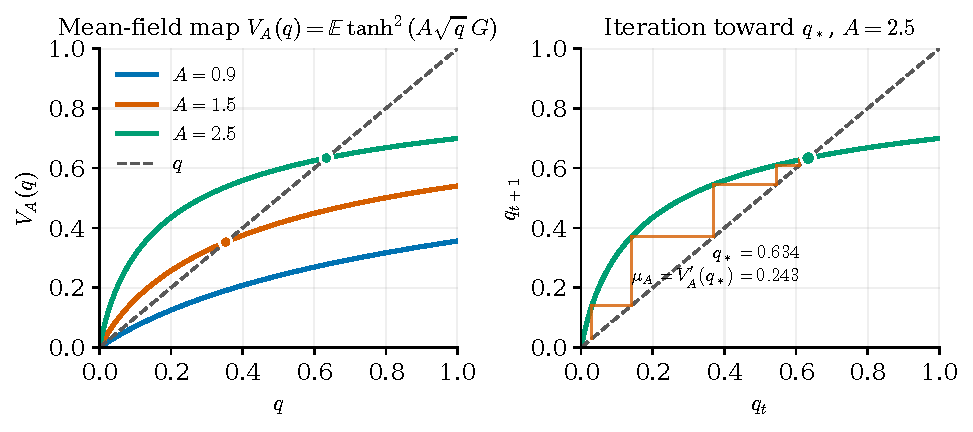
\includegraphics[width=\textwidth]{images/f5_meanfield}
  \caption{Unrounded squared-radius mean map. Left: $V_A$ and the diagonal for three
  gains; a positive fixed point appears for $A>1$. Right: iteration of $V_A$
  toward $q_\ast$ for $A=2.5$.}
  \label{fig:meanfield}
\end{figure}

\emph{Supercritical dimension cutoff.}
\Cref{fig:cutoff} shows the empirical
total variation distance $\norm{K_{A,N}^t(q_0,\cdot)-\nu_{A,N}}_{\TV}$ of the
unrounded squared-radius chain to its nonzero invariant law, plotted against the centered time
$t-t_N(q_0)$ for a range of widths $N$. The curves stay near one before the
cutoff time and drop toward zero afterwards, consistently with
\cref{thm:gaussian-process-cutoff}. The dashed curves are heuristic local
Gaussian approximations to the finite-$N$ transition.

\begin{figure}[H]
  \centering
  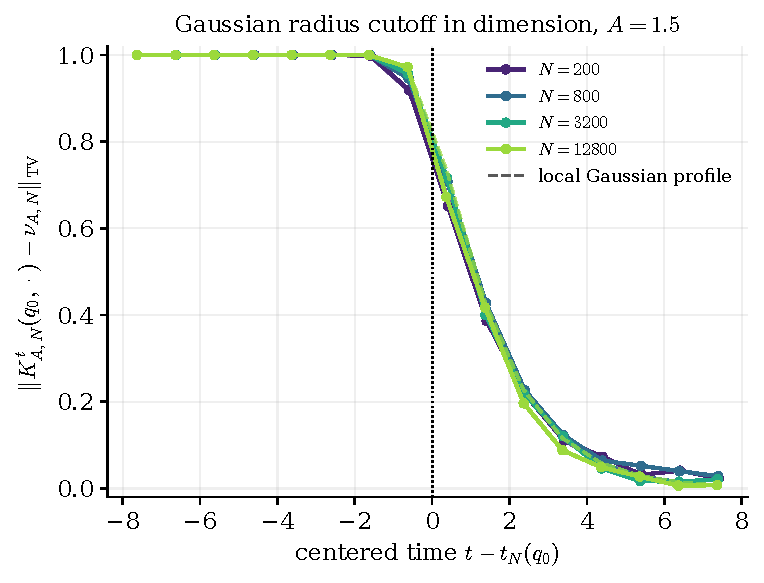
\includegraphics[width=0.66\textwidth]{images/f1_cutoff}
  \caption{Numerical supercritical dimension cutoff for the unrounded
  squared-radius chain, with $A=1.5$ and $q_0=0.05$. The solid curves are histogram estimates
  of the total variation distance to $\nu_{A,N}$ from $4{,}000$ simulated
  paths. The dashed curves are heuristic local Gaussian approximations.}
  \label{fig:cutoff}
\end{figure}

\emph{Invariant law and power-law singularity.}
In the supercritical regime, the unrounded vector chain has a nonzero invariant law
characterized by \cref{prop:nd-stationary-equation}. \Cref{fig:radiuslaw}
compares a long run of the unrounded radius chain with a numerical solution of a
discretized invariant equation. For $N=1$, the transition probabilities are
computed from the exact conditional distribution on a mesh refined near zero.
The logarithmic lower-tail plot also shows a
reference line with the Cram\'er slope $\beta_{A,N}$ from
\cref{thm:nd-power-singularity:intro}.

\begin{figure}[H]
  \centering
  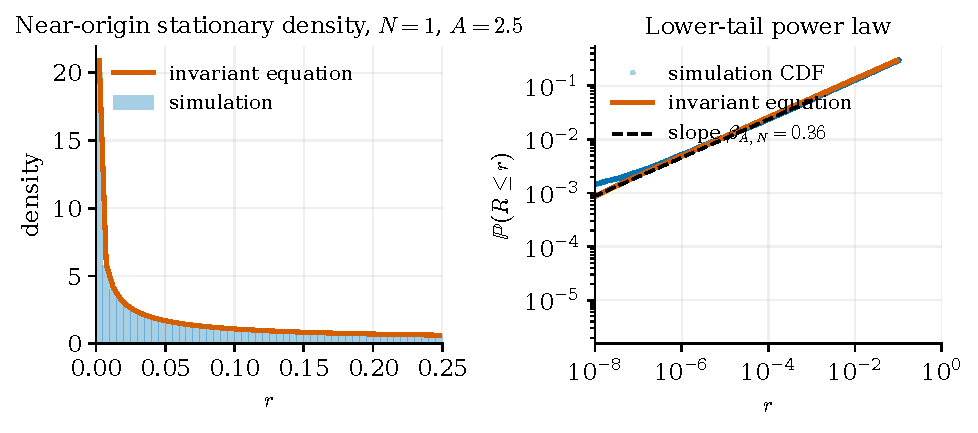
\includegraphics[width=\textwidth]{images/f2_radius_law}
  \caption{Supercritical stationary Euclidean radius for $N=1$ and $A=2.5$.
  Left: the near-origin density from simulation and a numerical solution of
  the invariant equation; the density increases toward zero because
  $\beta_{A,1}<1$. Right: the empirical and numerical lower tails and a reference line of
  slope $\beta_{A,1}$. The observed slope is consistent with
  \cref{thm:nd-power-singularity:intro}.}
  \label{fig:radiuslaw}
\end{figure}

\emph{Vanishing-mesh cutoff at fixed width.}
At fixed width and subcritical gain, \cref{eq:tv-absorption} identifies the
survival probability with the total variation distance to $\delta_0$.
\Cref{fig:precision} plots this probability on the theorem scale, with center
$L_\varrho/\gamma_{A,N}$ and window
$\sigma_N\gamma_{A,N}^{-3/2}\sqrt{L_\varrho}$. As $\varrho$ decreases, the
curves approach the Gaussian first-passage profile
$\Phi_{\mathrm G}(-a)$ of
\cref{thm:rounded-gaussian-nearest-cutoff,prop:rounded-gaussian-threshold-cutoff}.
For the smallest displayed $\varrho$, the figure also includes the
finite-window log-random-walk reference, which displays the lattice correction.

\begin{figure}[H]
  \centering
  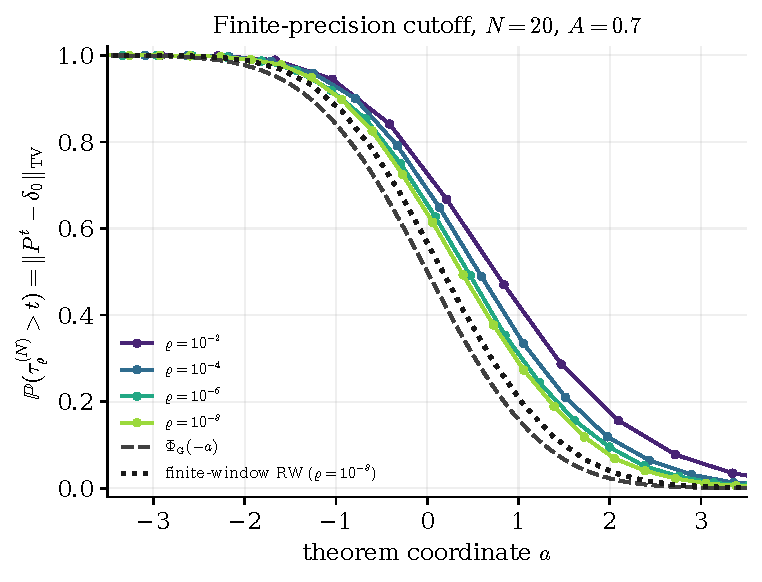
\includegraphics[width=0.66\textwidth]{images/f4_precision_cutoff}
  \caption{Vanishing-mesh cutoff at fixed width, with $N=20$ and $A=0.7$.
  The survival probability, equal to the total variation distance to
  $\delta_0$, is plotted using the center and window in
  \cref{thm:rounded-gaussian-nearest-cutoff}. The dashed curve is
  $\Phi_{\mathrm G}(-a)$; the dotted curve is the finite-window log-random-walk
  comparison at $\varrho=10^{-8}$.}
  \label{fig:precision}
\end{figure}

\emph{Fixed-precision cutoff in dimension.}
Fix the mesh size and let the dimension grow in the lattice-subcritical regime. For the
displayed parameters,
$A=0.7<A_{\mathrm{lat}}\approx0.8663$ and $\varrho=0.5$. By
\cref{thm:subcritical-dimension-cutoff}, the survival probability remains near
one at time $\bar t_N-1$ and is near zero by time $\bar t_N+2$, where
$\bar t_N$ is the first time at which the rounded deterministic orbit enters
the scale $(\log N)^{-1}$. \Cref{fig:subcritical-dimension-cutoff} plots the
empirical survival probability against the centered integer time
$t-\bar t_N$. The rounded squared-radius transition is sampled through its exact
finite-layer count distribution, which permits the large dimensions displayed in
the figure without changing the law of the rounded squared-radius chain.

\begin{figure}[H]
  \centering
  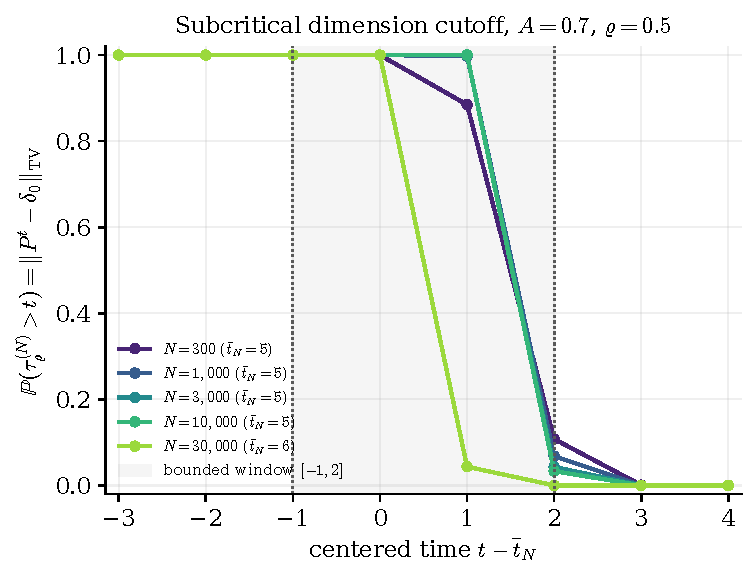
\includegraphics[width=0.66\textwidth]{images/f8_subcritical_dimension_cutoff}
  \caption{Fixed-precision subcritical dimension cutoff ($A=0.7$,
  $\varrho=0.5$, and $x_N=(1,\ldots,1)$; $40{,}000$ paths per dimension). The
  empirical survival probability
  $\Pp(\tau_\varrho^{(N)}>t)=
  \norm{P_{\varrho,A,N}^t(Q_\varrho x_N,\cdot)-\delta_0}_{\TV}$ is plotted
  against $t-\protect\bar t_N$. The dotted lines mark the lower and upper time
  bounds in \cref{thm:subcritical-dimension-cutoff}, namely
  $\protect\bar t_N-1$ and $\protect\bar t_N+2$.}
  \label{fig:subcritical-dimension-cutoff}
\end{figure}

\emph{Metastability in the bistable rounded regime.}
When the rounded squared-radius mean map has a positive stable fixed point separated
from the absorbing state by an unstable threshold
(\cref{prop:metastable-positive-fixed-points}), a large finite-width rounded vector chain
relaxes quickly toward the well and remains there for a long time before a
rare fluctuation triggers absorption. \Cref{fig:metastability}
shows the mean map, sample paths exhibiting the two time scales, and the
growth of the absorption time with width. The numerical behavior is consistent
with \cref{thm:rounded-qualitative-metastability}.

\begin{figure}[H]
  \centering
  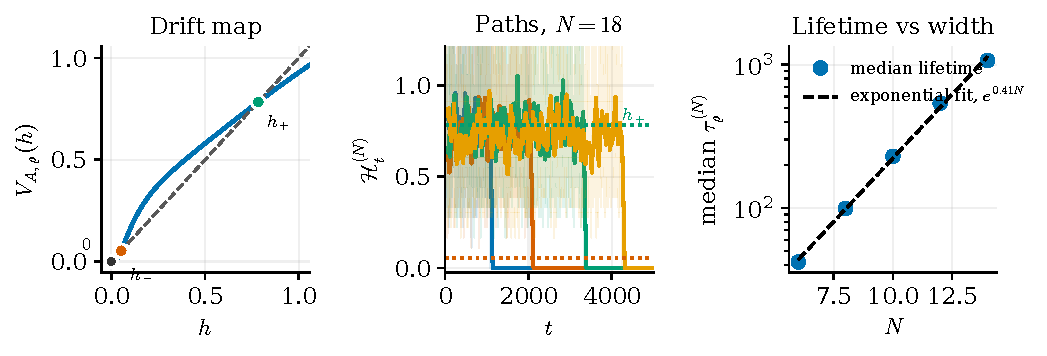
\includegraphics[width=\textwidth]{images/f3_metastability}
  \caption{Metastability for $A=1.15$ and $\varrho=0.5$. Left: the
  squared-radius mean map $V_{A,\varrho}$ with unstable endpoint $h_-$ and stable endpoint
  $h_+$. Middle: representative paths and moving averages with window $60$.
  Right: median absorption times and an exponential fit; the observed growth
  is consistent with \cref{thm:rounded-qualitative-metastability}.}
  \label{fig:metastability}
\end{figure}

\emph{Critical curves.}
\Cref{fig:thresholds} compares the fixed-width threshold $A_c(N)$ from
\cref{eq:fixed-width-critical}, which decreases to $1$, with the
fixed-precision thresholds $A_{\mathrm{lat}}$ and
$A_{\mathrm{ex}}(\varrho)$.

\begin{figure}[H]
  \centering
  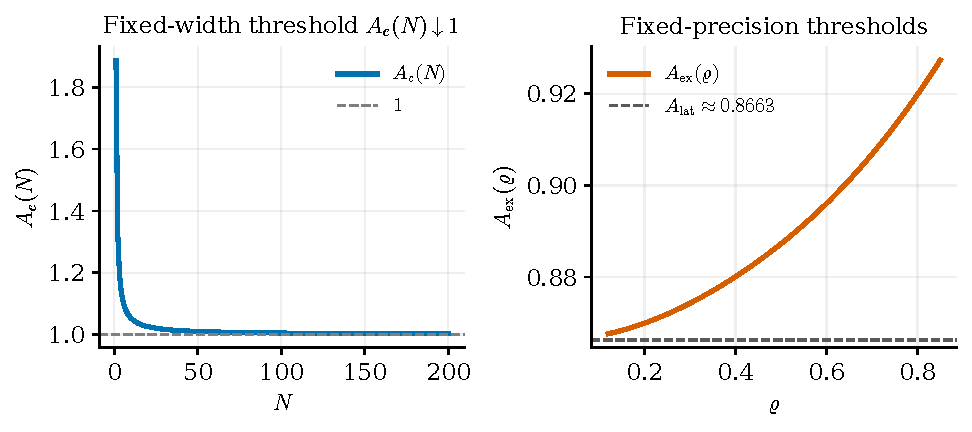
\includegraphics[width=\textwidth]{images/f7_thresholds}
  \caption{Threshold comparison. Left: the fixed-width critical gain
  $A_c(N)$ decreases to $1$. Right: the positive-fixed-point existence
  threshold $A_{\mathrm{ex}}(\varrho)$, evaluated numerically from its
  variational definition, and the lattice-contraction threshold
  $A_{\mathrm{lat}}$.}
  \label{fig:thresholds}
\end{figure}


\clearpage
\appendix

\section{Common probabilistic estimates}
\label{app:common-probabilistic-estimates}

This appendix proves
\cref{lem:common-stopped-orbit-tracking,lem:negative-drift-affine-entrance}
and
\cref{prop:gaussian-compactness-selection,prop:gaussian-nonzero-invariant-existence}.

\subsection{Stopped orbit tracking}
\label{app:common-stopped-orbit-tracking}

\begin{proof}[Proof of \cref{lem:common-stopped-orbit-tracking}]
  Put $T:=T_N$ and suppress the index $N$ on $\mathcal R_t$, $A_t$,
  $\eta_t$, $\alpha_t$, and $\sigma_t$ throughout the proof.

  \emph{Step 1: The killed moment.}
  Fix $0\leq t<T$. Since $\tau_N$ is a stopping time,
  $\{\tau_N>t\}\in\mathcal F_t$. Moreover,
  $\{\tau_N>t+1\}\subseteq\{\tau_N>t\}$, and on the latter event the
  recursion \cref{eq:common-tracking-recursion} applies. Consequently,
  \begin{equation*}
    \mathcal R_{t+1}^2\one_{\{\tau_N>t+1\}}
    \leq
    \one_{\{\tau_N>t\}}
    (A_t\mathcal R_t+\eta_{t+1})^2.
  \end{equation*}
  The variables $\one_{\{\tau_N>t\}}$, $A_t$, and $\mathcal R_t$ are
  $\mathcal F_t$-measurable. Thus the conditional cross term vanishes by
  \cref{eq:common-tracking-noise}, and
  \begin{equation*}
    \Ee\left[
      \mathcal R_{t+1}^2\one_{\{\tau_N>t+1\}}
      \,\middle|\,\mathcal F_t
    \right]
    \leq
    \one_{\{\tau_N>t\}}
    \left(
      A_t^2\mathcal R_t^2
      +\Ee[\eta_{t+1}^2\mid\mathcal F_t]
    \right)
    \leq
    \one_{\{\tau_N>t\}}
    \left(
      \alpha_t^2\mathcal R_t^2
      +\frac{C\sigma_t^2}{N}
    \right).
  \end{equation*}
  Set
  $m_t:=\Ee[\mathcal R_t^2\one_{\{\tau_N>t\}}]$. Taking expectations in
  the preceding display and using $\Pp(\tau_N>t)\leq1$ gives
  \begin{equation*}
    m_{t+1}
    \leq
    \alpha_t^2m_t+\frac{C\sigma_t^2}{N}.
  \end{equation*}
  Iterating this deterministic recursion, and using
  $m_0\leq\Ee\mathcal R_0^2$, yields
  \begin{equation*}
    m_t
    \leq
    \left(\prod_{u=0}^{t-1}\alpha_u^2\right)
    \Ee\mathcal R_0^2
    +\frac{C}{N}\sum_{s=0}^{t-1}
    \sigma_s^2\prod_{u=s+1}^{t-1}\alpha_u^2.
  \end{equation*}
  This is \cref{eq:common-killed-orbit-tracking}.

  \emph{Step 2: The stopped moment.}
  Define the deterministic backward weights
  \begin{equation*}
    W_t:=\prod_{u=t}^{T-1}(1\vee\alpha_u^2),
    \qquad 0\leq t\leq T.
  \end{equation*}
  These weights satisfy
  \begin{equation*}
    W_T=1,
    \qquad
    W_{t+1}\leq W_t,
    \qquad
    \alpha_t^2W_{t+1}\leq W_t.
  \end{equation*}
  In addition, the definition of $K_N$ gives
  \begin{equation*}
    W_0^{1/2}
    =\prod_{u=0}^{T-1}(1\vee\alpha_u)
    \leq K_N,
    \qquad
    \sigma_tW_{t+1}^{1/2}
    =\sigma_t\prod_{u=t+1}^{T-1}(1\vee\alpha_u)
    \leq K_N.
  \end{equation*}

  For the one-step weighted estimate, note that on
  $\{\tau_N\leq t\}$ the stopped process is constant, whereas on
  $\{\tau_N>t\}$ the recursion applies. Hence
  \begin{equation*}
    \overline{\mathcal R}_{t+1,N}
    =
    \one_{\{\tau_N\leq t\}}\overline{\mathcal R}_{t,N}
    +
    \one_{\{\tau_N>t\}}(A_t\mathcal R_t+\eta_{t+1}).
  \end{equation*}
  The two events in this decomposition are disjoint. Taking conditional
  expectations, using \cref{eq:common-tracking-noise}, and applying the
  preceding bounds therefore gives
  \begin{align*}
    &\Ee\left[
      W_{t+1}\overline{\mathcal R}_{t+1,N}^2
      \,\middle|\,\mathcal F_t
    \right]
    \\
    &\quad=
    \one_{\{\tau_N\leq t\}}W_{t+1}
      \overline{\mathcal R}_{t,N}^2
    +
    \one_{\{\tau_N>t\}}W_{t+1}
      \left(A_t^2\mathcal R_t^2
      +\Ee[\eta_{t+1}^2\mid\mathcal F_t]\right)
    \\
    &\quad\leq
    \one_{\{\tau_N\leq t\}}W_t
      \overline{\mathcal R}_{t,N}^2
    +
    \one_{\{\tau_N>t\}}W_t\mathcal R_t^2
    +\frac{CK_N^2}{N}
    \\
    &\quad=
    W_t\overline{\mathcal R}_{t,N}^2
    +\frac{CK_N^2}{N}.
  \end{align*}
  Taking expectations and using the tower property gives, for every
  $0\leq t<T$,
  \begin{equation*}
    \Ee\left[W_{t+1}\overline{\mathcal R}_{t+1,N}^2\right]
    -\Ee\left[W_t\overline{\mathcal R}_{t,N}^2\right]
    \leq
    \frac{CK_N^2}{N}.
  \end{equation*}
  Summing from $t=0$ to $T-1$, the left-hand side telescopes, and we obtain
  \begin{equation*}
    \Ee\left[W_T\overline{\mathcal R}_{T,N}^2\right]
    -\Ee\left[W_0\overline{\mathcal R}_{0,N}^2\right]
    \leq
    \frac{CK_N^2T}{N}.
  \end{equation*}
  Since $W_T=1$, $W_0$ is deterministic, and
  $\overline{\mathcal R}_{0,N}=\mathcal R_{0,N}$, this is equivalent to
  \begin{equation*}
    \Ee\overline{\mathcal R}_{T,N}^2
    \leq
    W_0\Ee\mathcal R_{0,N}^2+\frac{CK_N^2T}{N}.
  \end{equation*}
  Since $W_0\leq K_N^2$, this proves
  \cref{eq:common-stopped-orbit-tracking}.

  \emph{Step 3: Exit probability.}
  Suppose that $\tau_N$ is the first time at which
  $\abs{\mathcal R_{t,N}}>\delta$. On $\{\tau_N\leq T_N\}$ we have
  $T_N\wedge\tau_N=\tau_N$. Therefore, by the definition of
  the stopped process and the strict inequality in the definition of
  $\tau_N$,
  \begin{equation*}
    \overline{\mathcal R}_{T_N,N}
    =\mathcal R_{\tau_N,N},
    \qquad
    \abs{\mathcal R_{\tau_N,N}}>\delta.
  \end{equation*}
  Hence
  \begin{equation*}
    \delta^2\one_{\{\tau_N\leq T_N\}}
    \leq
    \overline{\mathcal R}_{T_N,N}^2.
  \end{equation*}
  Taking expectations and applying
  \cref{eq:common-stopped-orbit-tracking}, we obtain
  \begin{align*}
    \delta^2\Pp(\tau_N\leq T_N)
    &=
    \delta^2\Ee\one_{\{\tau_N\leq T_N\}}
    \\
    &\leq
    \Ee\overline{\mathcal R}_{T_N,N}^2
    \\
    &\leq
    CK_N^2\left(
      \Ee\mathcal R_{0,N}^2+\frac{T_N}{N}
    \right).
  \end{align*}
  Dividing by $\delta^2$ proves \cref{eq:common-orbit-exit-bound} and
  completes the proof.
\end{proof}

\subsection{Negative-drift affine entrance}
\label{app:common-affine-entrance}

\begin{proof}[Proof of \cref{lem:negative-drift-affine-entrance}]
  By our assumptions we can choose $\eps>0$ so small that
  $\mu_\eps:=\Ee\log(M_1+\eps)<0$. Take $K_\ast\geq b/\eps$. Whenever
  $U_t\geq K_\ast$,
  \begin{equation*}
    U_{t+1}
    =
    M_{t+1}U_t+b
    \leq
    M_{t+1}U_t+\eps K_\ast
    \leq
    (M_{t+1}+\eps)U_t .
  \end{equation*}
  Let $T:=\inf\{t:U_t\leq K_\ast\}$. On the event $\{T>n\}$ we have
  $U_t>K_\ast$ for every $t\leq n$, so the previous bound applies at each step
  and
  \begin{equation*}
    \log U_n\leq\log K+\widetilde S_n,
    \qquad
    \widetilde S_n:=\sum_{j=1}^n\log(M_j+\eps),
  \end{equation*}
  a random walk with increment mean $\mu_\eps<0$. Since $U_n>K_\ast$ on
  $\{T>n\}$, this forces $\widetilde S_n>-\log(K/K_\ast)$.

  By hypothesis $\log(M_1+\eps)$ has exponential moments near the origin, so
  $\Lambda(s):=\log\Ee(M_1+\eps)^s$ is finite for $s$ in a neighborhood of $0$,
  with $\Lambda(0)=0$ and $\Lambda'(0)=\mu_\eps<0$. Fix $s>0$ small enough that
  $\Lambda(s)<0$ and put $c_3:=-\Lambda(s)>0$. Chernoff's inequality gives, for
  every integer $n\geq1$,
  \begin{equation*}
    \Pp(T>n)
    \leq
    \Pp\!\left(\widetilde S_n>-\log(K/K_\ast)\right)
    \leq
    \left(\frac K{K_\ast}\right)^{s}\left(\Ee(M_1+\eps)^s\right)^{n}
    =
    \left(\frac K{K_\ast}\right)^{s}e^{-c_3n}.
  \end{equation*}
  Since $T$ is integer valued,
  $\Pp(T>c_1\log K+r)=\Pp(T>\lfloor c_1\log K+r\rfloor)$, and using
  $\lfloor c_1\log K+r\rfloor>c_1\log K+r-1$ with the choice $c_1:=s/c_3$,
  \begin{equation*}
    \Pp(T>c_1\log K+r)
    \leq
    \left(\frac K{K_\ast}\right)^{s}e^{c_3}e^{-c_3(c_1\log K+r)}
    =
    K_\ast^{-s}e^{c_3}\,K^{s-c_3c_1}e^{-c_3r}
    =
    K_\ast^{-s}e^{c_3}e^{-c_3r},
  \end{equation*}
  because $s-c_3c_1=0$. This is \cref{eq:negative-drift-affine-entrance} with
  $c_2:=\max\{K_\ast^{-s}e^{c_3},1\}$.
\end{proof}

\subsection{Compactness and invariant-law selection}
\label{app:common-invariant-law}

\begin{proof}[Proof of \cref{prop:gaussian-compactness-selection}]
  This is the Markov-kernel analogue of the classical Krylov--Bogolyubov
  averaging construction; compare \cite{kryloff-bogoliouboff1937}.
  The space $[0,1]$ is compact, and hence the set of probability measures on
  $[0,1]$ is weakly compact. The transition kernel is
  Feller: if $\phi$ is continuous and bounded on $[0,1]$, then
  \begin{equation*}
    K_{A,N}\phi(q)
    =
    \int_{\R^N}
    \phi\left(F_{A,N}(q,g)\right)\,\mathcal G_N(\mathrm{d}g)
  \end{equation*}
  is continuous in $q$, by the continuity of $F_{A,N}$ and dominated
  convergence.

  Let $\overline\nu_{T_j}^{\,q}\Rightarrow\overline\nu$. For every continuous
  $\phi$,
  \begin{align*}
    \overline\nu_{T_j}^{\,q}K_{A,N}\phi
    -
    \overline\nu_{T_j}^{\,q}\phi
    &=
    \frac1{T_j}
    \left(
      K_{A,N}^{T_j}\phi(q)-\phi(q)
    \right).
  \end{align*}
  The right-hand side tends to zero. Passing to the limit, using the Feller
  property for $K_{A,N}\phi$, gives
  $\overline\nu K_{A,N}\phi=\overline\nu\phi$ for every continuous $\phi$.
  Thus $\overline\nu$ is invariant.
  The weak stationary equation
  \cref{eq:gaussian-q-stationary-equation} follows by identification with continuous
  functions since $[0,1]$ is compact.

  Since $K_{A,N}(0,\cdot)=\delta_0$ and
  $K_{A,N}(s,\{0\})=0$ for $s>0$ (all Gaussian coordinates would have to
  vanish), an invariant law
  $\overline\nu\neq\delta_0$ decomposes as
  \begin{equation*}
    \overline\nu
    =
    \overline\nu(\{0\})\delta_0
    +
    \left(1-\overline\nu(\{0\})\right)\nu^+,
  \end{equation*}
  with $\nu^+$ invariant on $(0,1]$. The assertion for the vector law is then
  exactly the invariant-law part of \cref{prop:gaussian-tv-reduction}; the weak
  equation \cref{eq:gaussian-vector-weak-stationary-equation} is the
  corresponding stationary equation for the unrounded vector chain.
\end{proof}

\subsection{Nonzero invariant-law existence}
\label{app:common-nonzero-invariant-existence}

Let
$G_1,\ldots,G_N$ be independent standard Gaussians and put
\begin{equation*}
  S_N:=\frac1N\sum_{i=1}^N\min(G_i^2,1).
\end{equation*}
If $0 < u < 1/N$, then $S_N\leq u$ implies
$\abs{G_i}\leq\sqrt{Nu}$ for every $i$. Hence
\begin{equation*}
  \Pp(S_N\leq u)
  \leq
  \prod_{i=1}^N\Pp(\abs{G_i}\leq\sqrt{Nu})
  \leq
  C_N u^{N/2}.
\end{equation*}
Consequently, $\Ee S_N^{-p}<\infty$ for every $p<N/2$.


\begin{proof}[Proof of \cref{prop:gaussian-nonzero-invariant-existence}]
  Since $A>A_c(N)$,
  \begin{equation*}
    \frac{d}{dp} \Ee\left[
      \left(A^2\frac{\chi_N^2}{N}\right)^{-p}
    \right]_{p=0}
    =
    -\Ee\log\left(A^2\frac{\chi_N^2}{N}\right)
    =2\gamma_{A,N}<0,
  \end{equation*}
  where $\ell_{A,N}$ is as in
  \cref{eq:gaussian-linearized-radius-multiplier}, and
  $\gamma_{A,N}=-\Ee\log\ell_{A,N}<0$ in the present supercritical regime.
  Therefore there exists $p\in(0,N/2)$ such that
  \begin{equation}\label{eq:gaussian-simple-linear-negative-moment}
    \Ee\left[
      \left(A^2\frac{\chi_N^2}{N}\right)^{-p}
    \right]
    <1 .
  \end{equation}
  We claim that, for some $R_0\in(0,1)$ and $a<1$,
  \begin{equation}\label{eq:gaussian-simple-near-zero-drift}
    \sup_{0<r\leq R_0}
    \Ee\left[
      \left(\frac{F_{A,N}(r,G)}{r}\right)^{-p}
    \right]
    \leq a .
  \end{equation}
  Indeed, for fixed $g$ the quotient
  $q^{-1}\tanh^2(A\sqrt q\,g)$ decreases in $q$ and converges to
  $A^2g^2$ as $q\downarrow0$. Therefore
  $F_{A,N}(q,G)/q$ converges almost surely to
  $A^2\chi_N^2/N$. Moreover, for each fixed $R>0$ and $0<q\leq R$, the same
  monotonicity gives
  \begin{equation*}
    \frac{F_{A,N}(q,G)}q
    \geq
    \frac{F_{A,N}(R,G)}R .
  \end{equation*}
  The random variable on the right is bounded below by $c_{A,R,N}S_N$.
  The elementary fixed-$N$ small-ball estimate above gives
  $\Ee S_N^{-p}<\infty$. Dominated convergence therefore gives the convergence
  of the expectations, and \cref{eq:gaussian-simple-near-zero-drift} follows from
  \cref{eq:gaussian-simple-linear-negative-moment} by taking $R_0$ small.

  On the complementary region there is $B<\infty$ such that
  \begin{equation}\label{eq:gaussian-simple-outside-bound}
    \sup_{r\in[R_0,1]}\Ee F_{A,N}(r,G)^{-p}\leq B .
  \end{equation}
  This follows from the pointwise lower bound
  \begin{equation*}
    \tanh^2(A\sqrt r\,g)\geq c_{A,R_0}\min(g^2,1),
    \qquad r\in[R_0,1],
  \end{equation*}
  together with the same elementary fixed-$N$ small-ball estimate for $S_N$.

  Let $V(r):=r^{-p}$ for $r>0$. Combining the two estimates gives
  \begin{equation}\label{eq:gaussian-simple-foster}
    K_{A,N}V(r)\leq aV(r)+B,
    \qquad r>0.
  \end{equation}
  Let the unrounded squared-radius chain start from $q\in(0,1]$. Iterating
  \cref{eq:gaussian-simple-foster} gives
  \begin{equation*}
    \frac1T\sum_{t=0}^{T-1}\Ee V(Z_t^{(N)})
    \leq
    \frac{V(q)}{T(1-a)}+\frac{B}{1-a}.
  \end{equation*}
  Choose a weakly convergent Cesàro subsequence
  $\overline\nu_{T_j}^{\,q}\Rightarrow\overline\nu$. For
  $M<\infty$, the function $V^M(r):=\min\{r^{-p},M\}$ for $r>0$ and
  $V^M(0):=M$ is continuous on $[0,1]$. Passing to the limit gives a bound
  independent of $M$. Since
  $M\overline\nu(\{0\})\leq\int V^M\,\mathrm{d}\overline\nu$, letting
  $M\to\infty$ first gives $\overline\nu(\{0\})=0$. Monotone convergence on
  $(0,1]$ then gives
  \begin{equation*}
    \int_{(0,1]}r^{-p}\,\overline\nu(\mathrm{d}r)<\infty,
    \qquad
    \overline\nu(\{0\})=0.
  \end{equation*}
  Thus $\overline\nu\neq\delta_0$, and
  \cref{prop:gaussian-compactness-selection} shows that
  $\overline\nu\in\mathcal I_{A,N}^+(q)$. The vector invariant law follows
  from \cref{eq:gaussian-compactness-vector-law}.
\end{proof}

\section{Technical estimates for the supercritical dimension cutoff}
\label{app:supercritical-cutoff-estimates}

This appendix contains the estimates used in
\cref{subsec:gaussian-process-cutoff}, with the notation introduced there for
the unrounded squared-radius chain and its deterministic orbit.

\subsection{Negative moments and Foster estimates}
\label{app:supercritical-negative-moments}

\begin{proof}[Proof of \cref{lem:gaussian-truncated-cramer}]
  Let
  \begin{equation*}
    U_i:=\min(G_i^2,1),
    \qquad
    S_N:=\frac1N\sum_{i=1}^N U_i.
  \end{equation*}
  For $\lambda\geq1$,
  \begin{equation*}
    \Ee e^{-\lambda U_1}
    \leq
    \int_{-1}^1 e^{-\lambda x^2}\frac{e^{-x^2/2}}{\sqrt{2\pi}}\,\mathrm{d}x
    +
    e^{-\lambda}
    \leq
    C\lambda^{-1/2}.
  \end{equation*}
  Chernoff's bound with $\lambda=u^{-1}$ gives
  \begin{equation*}
    \Pp(S_N\leq u)
    \leq
    e^N
    \left(\Ee e^{-U_1/u}\right)^N
    \leq
    C^N u^{N/2},
  \end{equation*}
  for $0<u\leq1$.

  For $x,p>0$, the Gamma integral and the change of variables $v=ux$ give
  \begin{equation*}
    x^{-p}
    =
    \frac1{\Gamma(p)}
    \int_0^\infty u^{p-1}e^{-ux}\,\mathrm{d}u.
  \end{equation*}
  Let $p=\alpha N$ with $\alpha\in(0,1/2)$. By Tonelli's theorem and
  independence,
  \begin{align*}
    \Ee S_N^{-p}
    &=
    \frac1{\Gamma(p)}
    \int_0^\infty
    u^{p-1}
    \left(\Ee e^{-(u/N)U_1}\right)^N
    \,\mathrm{d}u .
  \end{align*}
  We split the integral at $u=N$. On $[0,N]$ we use the trivial bound
  $\Ee e^{-(u/N)U_1}\leq1$. On $[N,\infty)$ we use the preceding
  one-coordinate Laplace bound with $\lambda=u/N\geq1$. Since
  $p=\alpha N<N/2$, this gives
  \begin{align*}
    \Ee S_N^{-p}
    &\leq
    \frac{N^p}{\Gamma(p+1)}
    +
    \frac{C^N N^{N/2}}{\Gamma(p)}
    \int_N^\infty u^{p-1-N/2}\,\mathrm{d}u
    \\
    \leq
    C_\alpha^N
    \frac{N^p}{\Gamma(p+1)}.
  \end{align*}
  Stirling's formula, after increasing the constant to handle bounded $N$,
  shows that the last expression is bounded by $e^{C_\alpha N}$.
  If $W_{L,i}:=\min(G_i^2,L^2)$ and $L\geq1$, then $W_{L,i}\geq U_i$.
  Consequently,
  \begin{equation}\label{eq:gaussian-truncated-negative-moment}
    \sup_{L\geq1}
    \Ee\left[
      \left(
        \frac1N\sum_{i=1}^N W_{L,i}
      \right)^{-\alpha N}
    \right]
    \leq
    e^{C_\alpha N}.
  \end{equation}

  Put $\mu_L:=\Ee W_{L,1}$. Choose first $L$ large, then
  $\varepsilon>0$ small enough that $(1-\varepsilon)A^2\mu_L>1$, and finally
  $\delta>0$ such that
  \begin{equation*}
    a:=(1-\varepsilon)A^2(\mu_L-\delta)>1.
  \end{equation*}
  If $\overline W_{L,N}:=N^{-1}\sum_i W_{L,i}$, Hoeffding's inequality gives
  \begin{equation*}
    \Pp(\overline W_{L,N}<\mu_L-\delta)\leq e^{-c_0N}
  \end{equation*}
  with $c_0>0$ depending on $L$ and $\delta$.

  Fix $\alpha\in(0,1/2)$. By
  \cref{eq:gaussian-truncated-negative-moment}, after increasing
  $C_\alpha$ to absorb the fixed factor
  $((1-\varepsilon)A^2)^{-\alpha N}$,
  \begin{equation*}
    \Ee\left[
      \left((1-\varepsilon)A^2\overline W_{L,N}\right)^{-\alpha N}
    \right]
    \leq
    e^{C_\alpha N}.
  \end{equation*}
  On the event $\{\overline W_{L,N}\geq\mu_L-\delta\}$, the integrand in
  \cref{eq:gaussian-truncated-cramer} is at most $a^{-\gamma N}$. On the
  complementary event, Holder's inequality gives, for $0<\gamma<\alpha$,
  \begin{align*}
    \Ee\left[
      \left((1-\varepsilon)A^2\overline W_{L,N}\right)^{-\gamma N}
      \one_{\{\overline W_{L,N}<\mu_L-\delta\}}
    \right]
    &\leq
    e^{-c_0N(1-\gamma/\alpha)}
    e^{C_\alpha N\gamma/\alpha}.
  \end{align*}
  Choose $\gamma>0$ so small that
  $\gamma < \alpha c_0/(c_0+C_\alpha)$. Then choose $\kappa>0$ such that
  \begin{equation*}
    \kappa < \min\left\{
      \gamma\log a,
      c_0(1-\gamma/\alpha)-C_\alpha\gamma/\alpha
    \right\}.
  \end{equation*}
  The good- and bad-event estimates then give
  \cref{eq:gaussian-truncated-cramer}.
\end{proof}

\begin{proof}[Proof of \cref{prop:gaussian-near-zero-negative-moment}]
  Let $\gamma,\kappa,L,\varepsilon$ be as in
  \cref{lem:gaussian-truncated-cramer}, decreasing $\kappa$ if necessary.
  For $q>0$ define
  \begin{equation*}
    h_q(g)
    :=
    \frac{\tanh^2(A\sqrt q\,g)}{q}
    =
    A^2g^2
    \left(
      \frac{\tanh(A\sqrt q\,g)}{A\sqrt q\,g}
    \right)^2,
  \end{equation*}
  with the continuous interpretation at $g=0$. Since
  $x\mapsto \tanh x/x$ is decreasing on $(0,\infty)$, the map
  $q\mapsto h_q(g)$ is decreasing for each fixed $g$.

  Choose $R_0\in(0,\inf I_\ast)$ so small that
  \begin{equation}\label{eq:gaussian-ratio-lower-bound}
    \left(
      \frac{\tanh(A\sqrt{R_0}u)}{A\sqrt{R_0}u}
    \right)^2
    \geq
    1-\varepsilon
    \qquad \mbox{for every }\abs u\leq L.
  \end{equation}
  For $\abs g\leq L$, \cref{eq:gaussian-ratio-lower-bound} gives
  \begin{equation*}
    h_{R_0}(g)\geq(1-\varepsilon)A^2g^2.
  \end{equation*}
  For $\abs g>L$, the map
  $\abs g\mapsto h_{R_0}(g)=R_0^{-1}\tanh^2(A\sqrt{R_0}g)$ is increasing, and
  hence
  \begin{equation*}
    h_{R_0}(g)
    \geq
    h_{R_0}(L)
    \geq
    (1-\varepsilon)A^2L^2.
  \end{equation*}
  Therefore
  \begin{equation}\label{eq:gaussian-h-lower-truncated}
    h_{R_0}(g)
    \geq
    (1-\varepsilon)A^2\min(g^2,L^2)
    \qquad \mbox{for every }g\in\R.
  \end{equation}

  Hence, for $0<q\leq R_0$,
  \begin{equation*}
    \frac{F_{A,N}(q,G)}{q}
    =
    \frac1N\sum_{i=1}^N h_q(G_i)
    \geq
    \frac1N\sum_{i=1}^N h_{R_0}(G_i)
    \geq
    (1-\varepsilon)A^2
    \frac1N\sum_{i=1}^N\min(G_i^2,L^2).
  \end{equation*}
  Since $x\mapsto x^{-\gamma N}$ is decreasing on $(0,\infty)$, applying
  \cref{lem:gaussian-truncated-cramer} gives
  \begin{equation*}
    \sup_{0<q\leq R_0}
    \Ee\left[
      \left(
        \frac{F_{A,N}(q,G)}{q}
      \right)^{-\gamma N}
    \right]
    \leq
    e^{-\kappa N}
  \end{equation*}
  for all sufficiently large $N$.
\end{proof}

\begin{proof}[Proof of \cref{lem:gaussian-outside-negative-moment}]
  There is $c_{A,R_0}>0$ such that, for every $q\in[R_0,1]$ and every
  $g\in\R$,
  \begin{equation}\label{eq:gaussian-outside-pointwise-lower}
    \tanh^2(A\sqrt q\,g)
    \geq
    c_{A,R_0}\min(g^2,1).
  \end{equation}
  Indeed, for $\abs g\leq1$ this follows from the monotonicity of
  $\tanh x/x$ on $[0,A]$, while for $\abs g\geq1$ it follows from
  $\tanh^2(A\sqrt q\,\abs g)\geq\tanh^2(A\sqrt{R_0})$. Thus
  \begin{equation*}
    F_{A,N}(q,G)
    \geq
    c_{A,R_0}
    \frac1N\sum_{i=1}^N\min(G_i^2,1).
  \end{equation*}
  The bound follows from
  \cref{eq:gaussian-truncated-negative-moment}, after absorbing
  $c_{A,R_0}^{-\gamma N}$ into $e^{bN}$.
\end{proof}

\begin{proof}[Proof of \cref{prop:gaussian-stationary-negative-moment}]
  Let $R_0,\gamma,\kappa$ be as in
  \cref{prop:gaussian-near-zero-negative-moment}, and let $b$ be the constant
  in \cref{lem:gaussian-outside-negative-moment} for this choice of
  $R_0,\gamma$. Define
  \begin{equation*}
    V_N(q):=q^{-\gamma N},
    \qquad q>0.
  \end{equation*}
  For $q>0$, the two negative-moment estimates give the Foster inequality
  \begin{equation}\label{eq:gaussian-stationary-negative-moment-drift}
    K_{A,N}V_N(q)
    \leq
    e^{-\kappa N}V_N(q)+e^{bN}.
  \end{equation}
  Indeed, if $q\leq R_0$ then
  \begin{equation*}
    K_{A,N}V_N(q)
    =
    q^{-\gamma N}
    \Ee\left[\left(F_{A,N}(q,G)/q\right)^{-\gamma N}\right]
    \leq
    e^{-\kappa N}V_N(q),
  \end{equation*}
  while for $q\in[R_0,1]$ the outside estimate gives
  $K_{A,N}V_N(q)\leq e^{bN}$.

  Let $(Z_t^{(N)})_{t\geq0}$ be the unrounded squared-radius chain started from $1$. Iterating
  \cref{eq:gaussian-stationary-negative-moment-drift} yields
  \begin{equation}\label{eq:gaussian-stationary-negative-moment-iteration}
    \Ee V_N(Z_t^{(N)})
    \leq
    e^{-\kappa Nt}
    +
    \frac{e^{bN}}{1-e^{-\kappa N}}.
  \end{equation}
  Hence
  \begin{equation}\label{eq:gaussian-stationary-negative-moment-cesaro-bound}
    \int V_N(q)\,\overline\nu_T^{\,1}(\mathrm{d}q)
    \leq
    \frac{1}{T(1-e^{-\kappa N})}
    +
    \frac{e^{bN}}{1-e^{-\kappa N}}.
  \end{equation}
  Here $\overline\nu_T^{\,1}$ is the Cesàro average started from $q=1$ in
  \cref{eq:gaussian-cesaro-selection}.

  Take a weakly convergent subsequence
  $\overline\nu_{T_j}^{\,1}\Rightarrow\overline\nu$ with $T_j\to\infty$.
  For $M<\infty$ put $V_N^M(q):=\min\{V_N(q),M\}$ for $q>0$ and
  $V_N^M(0):=M$. Then $V_N^M$ is continuous on $[0,1]$. Applying
  \cref{eq:gaussian-stationary-negative-moment-cesaro-bound} with $T=T_j$ and
  then letting $j\to\infty$, the term containing $T_j^{-1}$ vanishes and
  \begin{equation*}
    \int V_N^M(q)\,\overline\nu(\mathrm{d}q)
    \leq
    \frac{e^{bN}}{1-e^{-\kappa N}}.
  \end{equation*}
  Letting $M\to\infty$ and using monotone convergence, we obtain
  $\int_{(0,1]}q^{-\gamma N}\,\overline\nu(\mathrm{d}q)<\infty$ and
  $\overline\nu(\{0\})=0$. By \cref{prop:gaussian-compactness-selection},
  $\overline\nu$ is a nonzero invariant law. By
  \cref{prop:gaussian-unique-nonzero-invariant},
  $\overline\nu=\nu_{A,N}$. The same monotone-convergence passage gives
  \cref{eq:gaussian-stationary-negative-moment}.
\end{proof}

\subsection{Localization, total variation, and concentration}
\label{app:supercritical-localization-concentration}

\begin{proof}[Proof of \cref{prop:gaussian-stable-localization}]
  Let $R_0,\gamma$ be as in
  \cref{prop:gaussian-near-zero-negative-moment}, and let $b$ be the constant
  from \cref{lem:gaussian-outside-negative-moment} for this choice of
  $R_0,\gamma$. Set
  \begin{equation*}
    V_N(q):=q^{-\gamma N},
    \qquad q>0.
  \end{equation*}
  By \cref{prop:gaussian-stationary-negative-moment}, after increasing $C$ if
  necessary,
  \begin{equation}\label{eq:gaussian-lyapunov-moment-bound}
    \int_0^1 V_N(q)\,\nu_{A,N}(\mathrm{d}q)
    \leq
    C e^{bN}.
  \end{equation}

  Now choose a second threshold $r\in(0,R_0)$ so small that
  \begin{equation}\label{eq:gaussian-final-threshold-choice}
    b+\gamma\log r<0.
  \end{equation}
  Since $V_N(q)\geq r^{-\gamma N}$ on $(0,r]$,
  \begin{equation}\label{eq:gaussian-small-mass-bound}
    \nu_{A,N}((0,r])
    \leq
    r^{\gamma N}
    \int_0^1 V_N(q)\,\nu_{A,N}(\mathrm{d}q)
    \leq
    C e^{-cN}.
  \end{equation}

  For the fixed-time entrance from $[r,1]$ into $I_\ast$, note that by
  \cref{lem:gaussian-mean-field-concavity}, every unrounded deterministic orbit started
  from $[r,1]$ converges monotonically to $q_\ast$ without crossing it.
  Hence
  \begin{equation*}
    \abs{V_A^{t+1}(q)-q_\ast}
    \leq
    \abs{V_A^t(q)-q_\ast},
    \qquad q\in[r,1].
  \end{equation*}
  Dini's theorem shows that this convergence is uniform on $[r,1]$.
  Therefore there are $m\in\N$ and $\eta>0$ such that
  \begin{equation}\label{eq:gaussian-deterministic-fixed-entrance}
    V_A^m([r,1])
    \subset
    I_{\ast,-\eta}
    :=
    \left\{
      q\in I_\ast:\operatorname{dist}(q,I_\ast^c)\geq\eta
    \right\}.
  \end{equation}
  Let $L<\infty$ be a Lipschitz constant for $V_A$ on $[0,1]$ and set
  \begin{equation*}
    \eta_m:=\frac{\eta}{2(1+L+\cdots+L^{m-1})}.
  \end{equation*}
  If the noise variables in \cref{eq:gaussian-noise-decomposition} have
  absolute value at most $\eta_m$ during the first $m$ steps, then the
  stochastic radius at time $m$ is within $\eta/2$ of its deterministic
  counterpart and hence belongs to $I_\ast$. Hoeffding's inequality
  \cref{eq:gaussian-noise-hoeffding} and a union bound over these fixed
  $m$ steps give
  \begin{equation}\label{eq:gaussian-fixed-time-entrance}
    \sup_{q\in[r,1]}
    K_{A,N}^m(q,I_\ast^c)
    \leq
    C e^{-cN}.
  \end{equation}

  Since $\nu_{A,N}$ is invariant,
  \begin{equation*}
    \nu_{A,N}(I_\ast^c)
    =
    \int_0^1 K_{A,N}^m(q,I_\ast^c)\,\nu_{A,N}(\mathrm{d}q)
    \leq
    \nu_{A,N}((0,r])
    +
    \sup_{q\in[r,1]}K_{A,N}^m(q,I_\ast^c).
  \end{equation*}
  Combining \cref{eq:gaussian-small-mass-bound,eq:gaussian-fixed-time-entrance}
  proves \cref{eq:gaussian-stationary-exponential-localization}, and the
  weaker estimate \cref{eq:gaussian-stationary-localization} follows
  immediately.
\end{proof}

\begin{proof}[Proof of \cref{lem:gaussian-score-smoothing}]
  Let $\mu_q$ be the law of $Y_q:=\tanh^2(A\sqrt q\,G)$ on $(0,1)$, and let
  $f_q$ be the density in \cref{eq:gaussian-one-coordinate-density}.
  Its $q$-score is
  \begin{equation}\label{eq:gaussian-one-coordinate-score}
    \ell_q(y)
    :=
    \partial_q\log f_q(y)
    =
    -\frac1{2q}
    +
    \frac{\arctanh(\sqrt y)^2}{2A^2q^2}.
  \end{equation}
  Since
  $\arctanh(\sqrt{Y_q})=\abs{A\sqrt q\,G}$, we have
  \begin{equation}\label{eq:gaussian-score-moments}
    \ell_q(Y_q)=\frac{G^2-1}{2q},
    \qquad
    \Ee \ell_q(Y_q)=0,
    \qquad
    \Ee \ell_q(Y_q)^2=\frac1{2q^2}.
  \end{equation}
  Fix a compact subinterval $I=[q_-,q_+]\Subset(0,1)$. On this interval the
  displayed density is a $C^1$ map into $L^1((0,1))$: after writing
  $u=\arctanh(\sqrt y)$, the substitution $y=\tanh^2u$ gives a
  uniform integrable Gaussian envelope for $\partial_qf_q=\ell_qf_q$. Thus
  $q\mapsto\mu_q$ is differentiable in total variation on $I$, with signed
  derivative measure $\partial_q\mu_q=\ell_q\mu_q$. Here and below
  $\abs\lambda$ denotes the total variation measure of a signed measure
  $\lambda$; with our convention for total variation distance between
  probability measures, one divides the signed variation norm by two.

  Let $Y_{1,q},\ldots,Y_{N,q}$ be independent copies of $Y_q$ and set
  \begin{equation*}
    M_{N,q}:=\frac1N\sum_{i=1}^N Y_{i,q},
    \qquad
    S_{N,q}:=\sum_{i=1}^N\ell_q(Y_{i,q}).
  \end{equation*}
  The product family is therefore differentiable in total variation by the
  tensorized score calculation:
  \begin{equation}\label{eq:gaussian-product-score-derivative}
    \partial_q\mu_q^{\otimes N}
    =
    S_{N,q}\,\mu_q^{\otimes N};
  \end{equation}
  equivalently, for every bounded measurable $\varphi:(0,1)^N\to\R$,
  \begin{equation}\label{eq:gaussian-score-test-function}
    \partial_q\Ee\varphi(Y_{1,q},\ldots,Y_{N,q})
    =
    \Ee\left[
      \varphi(Y_{1,q},\ldots,Y_{N,q})S_{N,q}
    \right].
  \end{equation}
  Since $S_{N,q}$ is the density of $\partial_q\mu_q^{\otimes N}$ against
  $\mu_q^{\otimes N}$, its total variation norm is
  \begin{equation}\label{eq:gaussian-score-product-bound}
    \abs{\partial_q\mu_q^{\otimes N}}((0,1)^N)
    =
    \Ee\abs{S_{N,q}}
    \leq
    \left(\Ee S_{N,q}^2\right)^{1/2}
    =
    \frac{\sqrt N}{\sqrt2\,q},
  \end{equation}
  where the last identity uses \cref{eq:gaussian-score-moments} and the
  independence of the $Y_{i,q}$.

  The squared-radius transition kernel $K_{A,N}(q,\cdot)$ is the law of
  $M_{N,q}$, that is, the
  pushforward of $\mu_q^{\otimes N}$ under the averaging map
  $(y_1,\ldots,y_N)\mapsto N^{-1}\sum_i y_i$; pushforward does not increase the
  total variation distance of probability measures. Since $q\mapsto\mu_q^{\otimes
  N}$ is continuously differentiable in total variation,
  $\mu_q^{\otimes N}-\mu_{q'}^{\otimes N}=\int_{q'}^q\partial_s\mu_s^{\otimes
  N}\,\mathrm{d}s$ as signed measures, so integrating
  \cref{eq:gaussian-score-product-bound} and halving,
  \begin{equation*}
    \norm{K_{A,N}(q,\cdot)-K_{A,N}(q',\cdot)}_{\TV}
    \leq
    \tfrac12\abs{\mu_q^{\otimes N}-\mu_{q'}^{\otimes N}}((0,1)^N)
    \leq
    \frac12\int_{q\wedge q'}^{q\vee q'}\frac{\sqrt N}{\sqrt2\,s}\,\mathrm{d}s
    \leq
    \frac{\sqrt N}{2\sqrt2\,q_-}\abs{q-q'} .
  \end{equation*}
  Since $q,q'\in I\Subset(0,1)$, this proves
  \cref{eq:gaussian-score-tv-smoothing} with $C_I=(2\sqrt2\,q_-)^{-1}$.
\end{proof}

\begin{proof}[Proof of \cref{prop:gaussian-stationary-concentration}]
  Invariance of $\nu_{A,N}$ and \cref{eq:gaussian-noise-moments} give
  \begin{align}
    \int_0^1 (q-q_\ast)^2\,\nu_{A,N}(\mathrm{d}q)
    &=
    \int_0^1
    \Ee\left[
      \left(F_{A,N}(q,G)-q_\ast\right)^2
    \right]
    \nu_{A,N}(\mathrm{d}q)
    \notag\\
    &=
    \int_0^1
    \left(V_A(q)-q_\ast\right)^2
    \nu_{A,N}(\mathrm{d}q)
    +
    O(N^{-1}).
    \label{eq:gaussian-stationary-concentration-step}
  \end{align}
  On $I_\ast$, \cref{eq:gaussian-stable-basin-derivative} gives
  $
    \abs{V_A(q)-q_\ast}
    \leq
    \kappa\abs{q-q_\ast}
  $.
  On $I_\ast^c$, we use the trivial bound
  $
    \abs{V_A(q)-q_\ast}\leq1
  $
  and \cref{eq:gaussian-stationary-localization}. Hence, if
  \begin{equation*}
    V_N:=
    \int_0^1 (q-q_\ast)^2\,\nu_{A,N}(\mathrm{d}q),
  \end{equation*}
  then
  $
    V_N
    \leq
    \kappa^2 V_N+\frac{C}{N}
  $.
  Since $\kappa<1$, this gives
  $
    V_N\leq \frac{C}{(1-\kappa^2)N}
  $.
  The claim follows after enlarging $C$.
\end{proof}

\begin{proof}[Proof of \cref{lem:gaussian-orbit-concentration}]
  \emph{Step 1: the finite-time entrance.}
  Put
  $
    e_t^{(N)}:=Z_t^{(N)}-q_{t,N}
  $.
  Since the comparison orbit starts from the same finite-$N$ radius
  $q_{0,N}$, one has $e_0^{(N)}=0$. Before $s_\ast$, no stability is
  needed: $V_A$ is Lipschitz on $[0,1]$, and
  \cref{eq:gaussian-noise-moments,eq:gaussian-noise-hoeffding} give, after
  finitely many iterations,
  \begin{equation}\label{eq:gaussian-entrance-error}
    \Ee[(e_{s_\ast}^{(N)})^2]\leq \frac{C}{N},
    \qquad
    \Pp\left(\abs{e_{s_\ast}^{(N)}}>\eta\right)
    \leq
    C\exp(-c_\eta N)
  \end{equation}
  for every fixed $\eta>0$.

  \emph{Step 2: The stopped second moment.}
  Use the one-step noise $\zeta_{t+1}^{(N)}$ and natural filtration
  $\mathcal F_t$ from
  \cref{eq:gaussian-noise-decomposition,eq:gaussian-noise-moments}. Then
  \begin{equation*}
    e_{t+1}^{(N)}
    =
    Z_{t+1}^{(N)}-q_{t+1,N}
    =
    V_A(Z_t^{(N)})-V_A(q_{t,N})
    +
    \zeta_{t+1}^{(N)}.
  \end{equation*}
  Moreover,
  \begin{equation*}
    \Ee[\zeta_{t+1}^{(N)}\mid \mathcal F_t]=0,
    \qquad
    \Ee[(\zeta_{t+1}^{(N)})^2\mid \mathcal F_t]\leq \frac{C}{N}.
  \end{equation*}

  On $\{t<\tau_\ast^{(N)}\}$, both $Z_t^{(N)}$ and $q_{t,N}$ lie in the
  stable interval $I_\ast$. Hence the mean value theorem and
  \cref{eq:gaussian-stable-basin-derivative} give
  \begin{equation*}
    \abs{V_A(Z_t^{(N)})-V_A(q_{t,N})}
    \leq
    \kappa\abs{e_t^{(N)}}.
  \end{equation*}
  Therefore, using the preceding decomposition and the martingale property of
  $\zeta_{t+1}^{(N)}$,
  \begin{equation*}
    \Ee\left[
      (e_{t+1}^{(N)})^2
      \,\middle|\,\mathcal F_t
    \right]
    =
    \left(
      V_A(Z_t^{(N)})-V_A(q_{t,N})
    \right)^2
    +
    \Ee\left[
      (\zeta_{t+1}^{(N)})^2
      \,\middle|\,\mathcal F_t
    \right]
    \leq
    \kappa^2(e_t^{(N)})^2+\frac{C}{N}
  \end{equation*}
  on $\{t<\tau_\ast^{(N)}\}$. Apply
  \cref{eq:common-killed-orbit-tracking} to the time-shifted process
  $(e_{s_\ast+j}^{(N)})_{j\geq0}$, with
  $\alpha_{j,N}=\kappa$ and $\sigma_{j,N}=C$. The geometric sum in that
  estimate is bounded by $(1-\kappa^2)^{-1}$, while
  \cref{eq:gaussian-entrance-error} supplies the $O(N^{-1})$ initial term.
  Hence
  \begin{equation}\label{eq:gaussian-stopped-orbit-concentration}
    \Ee\left[
      (e_t^{(N)})^2
      \one_{\{\tau_\ast^{(N)}>t\}}
    \right]
    \leq
    \frac{C}{N}.
  \end{equation}

  \emph{Step 3: No exit and removal of stopping.}
  Choose $\eta>0$ so small that
  \begin{equation*}
    \kappa\delta_\ast+\eta<\delta_\ast.
  \end{equation*}
  If
  \begin{equation*}
    \abs{e_{s_\ast}^{(N)}}\leq\eta
    \qquad\mbox{and}\qquad
    \abs{\zeta_j^{(N)}}\leq\eta
    \quad\mbox{for every }s_\ast<j\leq T_N,
  \end{equation*}
  then the recursion
  \begin{equation*}
    \abs{e_{t+1}^{(N)}}
    \leq
    \kappa\abs{e_t^{(N)}}+\abs{\zeta_{t+1}^{(N)}}
  \end{equation*}
  and the margin in \cref{eq:gaussian-deterministic-entrance} imply
  $Z_t^{(N)}\in I_\ast$ for every $s_\ast\leq t\leq T_N$. Hence
  \cref{eq:gaussian-noise-hoeffding,eq:gaussian-entrance-error} and a union
  bound give
  \begin{equation*}
    \Pp(\tau_\ast^{(N)}\leq T_N)
    \leq
    C T_N e^{-c_0N}.
  \end{equation*}

  Since $\abs{e_t^{(N)}}\leq1$, splitting according to whether the squared-radius chain has
  exited before time $t$ gives
  \begin{equation*}
    \Ee[(e_t^{(N)})^2]
    =
    \Ee\left[
      (e_t^{(N)})^2\one_{\{\tau_\ast^{(N)}>t\}}
    \right]
    +
    \Ee\left[
      (e_t^{(N)})^2\one_{\{\tau_\ast^{(N)}\leq t\}}
    \right]
    \leq
    \Ee\left[
      (e_t^{(N)})^2\one_{\{\tau_\ast^{(N)}>t\}}
    \right]
    +
    \Pp(\tau_\ast^{(N)}\leq t).
  \end{equation*}
  Combining this with
  \cref{eq:gaussian-stopped-orbit-concentration,eq:gaussian-orbit-no-exit} and
  $T_N=O(\log N)$ gives, uniformly for $t\leq T_N$,
  \begin{equation*}
    \Ee[(e_t^{(N)})^2]
    \leq
    \frac{C}{N}
    +
    C(\log N)e^{-c_0N}.
  \end{equation*}
  Multiplying by $N$ and increasing $C$ for finitely many small values of $N$
  proves \cref{eq:gaussian-orbit-concentration}.
\end{proof}

\subsection{Contraction at the cutoff scale}
\label{app:supercritical-cutoff-contraction}

\begin{proof}[Proof of \cref{lem:gaussian-synchronous-cutoff-scale}]
  \emph{Step 1: Setup.}
  Take $C_0$ as in \cref{eq:gaussian-uniform-log-horizon-constant} and fix
  $b>0$. All constants below are independent of $c$; the lower bound on $N$
  and the $o(1)$ terms may depend on its fixed value, which is harmless because
  the limit in $N$ is taken first. Fix $c\geq0$. By
  \cref{eq:gaussian-uniform-log-horizon},
  \begin{equation*}
    n_N(c)\leq C_0\log N
  \end{equation*}
  for all large $N$. The estimates from
  \cref{lem:gaussian-orbit-concentration} will be used only up to this time.
  For all sufficiently large $N$, put
  \begin{equation*}
    \ell_N:=\max\{0,\lfloor b\log\log N\rfloor\},
    \qquad
    s_N:=\max\{0,n_N(c)-1-\ell_N\}.
  \end{equation*}
  Since $n_N(c)-1-\ell_N>0$ eventually,
  $s_N+\ell_N=n_N(c)-1$ for all large $N$, and
  $\ell_N=o(\log N)$.
  Because $n_N(c)$ is of order $\log N$ while
  $\ell_N=o(\log N)$, we have $s_N\to\infty$. Hence, after increasing $N$ if
  necessary,
  \begin{equation*}
    s_N\geq s_\ast,
    \qquad
    0\leq s_N\leq s_N+\ell_N=n_N(c)-1\leq C_0\log N .
  \end{equation*}
  The orbit estimates from \cref{lem:gaussian-orbit-concentration} therefore
  apply at every time used in the last block.

  \emph{Step 2: Block-starting distance.}
  By the deterministic asymptotic in
  \cref{eq:gaussian-deterministic-asymptotic}, together with the definition of
  $t_N(q_0)$ and the bounded integer-time rounding in $n_N(c)$,
  \begin{equation}\label{eq:gaussian-block-deterministic-start}
    \abs{q_{s_N,N}-q_\ast}
    \leq
    C N^{-1/2}\mu_A^{c-\ell_N}
  \end{equation}
  for all large $N$, with $C$ independent of $c$. Indeed,
  \begin{equation*}
    s_N-\bigl(t_N(q_0)+c-\ell_N\bigr)\in[-2,-1],
  \end{equation*}
  so the rounding contributes at most the fixed factor $\mu_A^{-2}$; only the
  lower bound on $N$ in the locally uniform deterministic asymptotic may depend
  on $c$. Since $\widetilde Z_0^{(N)}\sim\nu_{A,N}$ and the law
  $\nu_{A,N}$ is invariant, also
  $\widetilde Z_{s_N}^{(N)}\sim\nu_{A,N}$. Therefore, by the triangle
  inequality, Cauchy's inequality,
  \cref{eq:gaussian-orbit-concentration}, and
  \cref{eq:gaussian-stationary-concentration},
  \begin{align*}
    \Ee\abs{Z_{s_N}^{(N)}-\widetilde Z_{s_N}^{(N)}}
    &\leq
    \Ee\abs{Z_{s_N}^{(N)}-q_{s_N,N}}
    +
    \abs{q_{s_N,N}-q_\ast}
    +
    \Ee\abs{\widetilde Z_{s_N}^{(N)}-q_\ast}
    \\
    &\leq
    C N^{-1/2}
    +
    C N^{-1/2}\mu_A^{c-\ell_N}
    +
    C N^{-1/2}.
  \end{align*}
  Hence
  \begin{equation}\label{eq:gaussian-block-start-distance}
    \Ee\abs{Z_{s_N}^{(N)}-\widetilde Z_{s_N}^{(N)}}
    \leq
    C N^{-1/2}\left(\mu_A^{c-\ell_N}+1\right).
  \end{equation}

  \emph{Step 3: Localizing the Block.}
  During the last $\ell_N$ steps, both squared-radius chains remain in a small neighborhood
  of $q_\ast$ with high probability. This localization is used only for the
  local Taylor contraction; the sharper size estimate is
  \cref{eq:gaussian-block-start-distance}. Let
  \begin{equation*}
    \rho_N:=(\log N)^{-2},
    \qquad
    J_N:=[q_\ast-\rho_N,q_\ast+\rho_N]\cap[0,1].
  \end{equation*}
  For every $0\leq j\leq\ell_N$, the unrounded deterministic orbit remains closer to
  $q_\ast$ as time increases. Hence \cref{eq:gaussian-block-deterministic-start}
  implies
  \begin{equation}\label{eq:gaussian-block-deterministic-local}
    q_{s_N+j,N}
    \in
    [q_\ast-\rho_N/2,q_\ast+\rho_N/2]
  \end{equation}
  for all large $N$, because
  $N^{-1/2}\mu_A^{c-\ell_N}=o(\rho_N)$. Chebyshev's inequality and
  \cref{eq:gaussian-orbit-concentration} therefore give
  \begin{equation*}
    \Pp\left(Z_{s_N+j}^{(N)}\notin J_N\right)
    \leq
    \Pp\left(
      \abs{Z_{s_N+j}^{(N)}-q_{s_N+j,N}}>\rho_N/2
    \right)
    \leq
    \frac{C}{N \rho_N^2}.
  \end{equation*}
  Similarly, stationarity of $\widetilde Z^{(N)}$ and
  \cref{eq:gaussian-stationary-concentration} imply
  \begin{equation*}
    \Pp\left(\widetilde Z_{s_N+j}^{(N)}\notin J_N\right)
    \leq
    \frac{C}{N \rho_N^2}.
  \end{equation*}
  Thus, with
  \begin{equation*}
    E_j
    :=
    \left\{
      Z_{s_N+j}^{(N)}\in J_N,\,
      \widetilde Z_{s_N+j}^{(N)}\in J_N
    \right\},
  \end{equation*}
  we have
  \begin{equation}\label{eq:gaussian-block-bad-probability}
    \Pp(E_j^c)
    \leq
    \frac{C}{N \rho_N^2}.
  \end{equation}

  \emph{Step 4: Local contraction.}
  On $J_N$ the deterministic map has derivative close to its derivative at
  $q_\ast$. Since $V_A'(q_\ast)=\mu_A$ and $V_A''$ is bounded in a
  neighborhood of $q_\ast$, the mean value theorem gives, for all large $N$
  and all $q,q'\in J_N$,
  \begin{equation}\label{eq:gaussian-local-taylor-contraction}
    \abs{V_A(q)-V_A(q')}
    \leq
    \left(\mu_A+C \rho_N\right)\abs{q-q'}.
  \end{equation}
  We choose $N$ large enough that
  $
    a_N:=\mu_A+C \rho_N<1
  $.

  Let
  $
    D_j:=
    \Ee |{
      Z_{s_N+j}^{(N)}
      -
      \widetilde Z_{s_N+j}^{(N)}
    } |
  $.
  \emph{Synchronous recursion.}
  Conditional on the two radii at time $s_N+j$, the next step uses the same
  Gaussian vector in both squared-radius chains. For fixed $g\in\R^N$, the map
  $q\mapsto F_{A,N}(q,g)$ is nondecreasing. Indeed, for $q>0$,
  \begin{equation*}
    \partial_q\tanh^2(A\sqrt q\,g_i)
    =
    \frac{Ag_i}{\sqrt q}
    \tanh(A\sqrt q\,g_i)
    \operatorname{sech}^2(A\sqrt q\,g_i)
    \geq0,
  \end{equation*}
  and the endpoint $q=0$ follows by continuity. Monotonicity therefore
  removes the absolute value inside the expectation, and for every
  $q,q'\in[0,1]$,
  \begin{equation*}
    \Ee\abs{F_{A,N}(q,G)-F_{A,N}(q',G)}
    =
    \abs{V_A(q)-V_A(q')}.
  \end{equation*}
  Applying this identity conditionally gives
  \begin{align*}
    \Ee\left[
      \abs{
        Z_{s_N+j+1}^{(N)}
        -
        \widetilde Z_{s_N+j+1}^{(N)}
      }
      \,\middle|\, Z_{s_N+j}^{(N)},\widetilde Z_{s_N+j}^{(N)}
    \right]
    =
    \abs{
      V_A(Z_{s_N+j}^{(N)})
      -
      V_A(\widetilde Z_{s_N+j}^{(N)})
    }.
  \end{align*}
  On $E_j$, \cref{eq:gaussian-local-taylor-contraction} bounds this
  by
  $a_N\abs{Z_{s_N+j}^{(N)}-\widetilde Z_{s_N+j}^{(N)}}$. On
  $E_j^c$ we use only the trivial bound by one. Taking expectations
  and using \cref{eq:gaussian-block-bad-probability} gives
  \begin{equation}\label{eq:gaussian-block-recursion}
    D_{j+1}
    \leq
    a_ND_j
    +
    \frac{C}{N \rho_N^2}
    \qquad
    0\leq j<\ell_N .
  \end{equation}

  Iterating the recursion and using $a_N<1$ gives
  \begin{equation*}
    D_{\ell_N}
    \leq
    a_N^{\ell_N}D_0
    +
    \frac{C}{N \rho_N^2}
    \sum_{k=0}^{\ell_N-1}a_N^k
    \leq
    a_N^{\ell_N}D_0
    +
    \frac{C}{N \rho_N^2}.
  \end{equation*}
  Since $\rho_N=(\log N)^{-2}$,
  \begin{equation*}
    \frac{1}{N \rho_N^2}
    =
    \frac{(\log N)^4}{N}
    =
    o(N^{-1/2}).
  \end{equation*}
  Hence
  \begin{equation}\label{eq:gaussian-block-iterated}
    D_{\ell_N}
    \leq
    a_N^{\ell_N}D_0
    +
    o(N^{-1/2}).
  \end{equation}

  \emph{Step 5: Terminal estimate.}
  The block length recovers the factor $\mu_A^{\ell_N}$, while the
  perturbation $C\rho_N$ has no asymptotic effect. Indeed,
  \begin{equation*}
    a_N^{\ell_N}
    =
    \mu_A^{\ell_N}
    \left(1+\frac{C \rho_N}{\mu_A}\right)^{\ell_N},
  \end{equation*}
  and $\ell_N \rho_N\to0$. Therefore
  \begin{equation}\label{eq:gaussian-block-factor}
    a_N^{\ell_N}
    =
    \mu_A^{\ell_N}(1+o(1)).
  \end{equation}
  Combining
  \cref{eq:gaussian-block-start-distance,eq:gaussian-block-iterated,eq:gaussian-block-factor}
  gives
  \begin{equation*}
    \sqrt N\,D_{\ell_N}
    \leq
    C\mu_A^{\ell_N}
    \left(\mu_A^{c-\ell_N}+1\right)
    +
    o(1)
    \leq
    C\mu_A^c+C\mu_A^{\ell_N}+o(1)
    =
    C\mu_A^c+o(1).
  \end{equation*}
  Here $\mu_A^{\ell_N}\to0$ because $\mu_A\in(0,1)$ and
  $\ell_N\to\infty$. The constants in the preceding estimate are independent
  of $c$, while the $o(1)$ term may depend on its fixed value.
  Since $D_{\ell_N}$ is the expectation in
  \cref{eq:gaussian-synchronous-cutoff-scale}, the claimed bound follows.
\end{proof}

\section*{Acknowledgements}
The author used OpenAI's ChatGPT~5.5 and Anthropic's Claude Opus~4.8 for
drafting, editing, and producing the accompanying Lean development through
agentic coding harnesses. The author supervised this work, reviewed the
resulting manuscript and formalization, and takes responsibility for their
contents.

\bibliographystyle{alpha}
\bibliography{refs}

\end{document}
